\documentclass{article}

\usepackage[utf8]{inputenc}

\usepackage{amsmath, bm}
\usepackage{graphicx}
\usepackage{amssymb}
\usepackage{float}
\usepackage{caption}
\usepackage{subcaption}
\usepackage{hyperref}
\usepackage{tikz}
\usepackage{layout}
\usepackage{booktabs}

\usepackage[margin=1in]{geometry}
\usepackage{listings}
\usepackage{xcolor}
\usepackage{color, colortbl}
\usepackage{textgreek}
\usepackage{mathrsfs}
\usepackage{savetrees}[moderate]
\usepackage{dirtree}
\usepackage{adjustbox}


\usetikzlibrary{calc}
\usetikzlibrary{angles,quotes} % for pic
\usetikzlibrary{patterns,snakes}
\usetikzlibrary{arrows}
\tikzset{>=latex} % for LaTeX arrow head

\setlength{\parskip}{\baselineskip}%
\setlength{\parindent}{0pt}%
\linespread{0.9}


\definecolor{codegreen}{rgb}{0,0.6,0}
\definecolor{codegray}{rgb}{0.5,0.5,0.5}
\definecolor{codepurple}{rgb}{0.58,0,0.82}
\definecolor{backcolour}{rgb}{0.95,0.95,0.92}

\lstdefinestyle{mystyle}{
    backgroundcolor=\color{backcolour},   
    commentstyle=\color{codegreen},
    keywordstyle=\color{magenta},
    numberstyle=\tiny\color{codegray},
    stringstyle=\color{codepurple},
    basicstyle=\ttfamily\footnotesize,
    breakatwhitespace=false,         
    breaklines=true,                 
    captionpos=b,                    
    keepspaces=true,                 
    numbers=left,                    
    numbersep=5pt,                  
    showspaces=false,                
    showstringspaces=false,
    showtabs=false,                  
    tabsize=2
}

\lstset{style=mystyle}



\begin{document}

\title{Computational Fluid Dynamics \\
    \large Final Report}
\author{lwp26}
\date{December 2024}
\maketitle 

\section{Introduction}

% make better
Computational Fluid Dynamics (CFD) is a powerful tool for solving fluid flow problems.
This can be done much faster and at lower cost than experimental methods.
This makes it a valuable tool to be used alongside experimental validation.


\section{Objectives}

%To write a program to solve the Euler equations for two-dimensional flows using a finite volume time
%marching method. Completing this work will give you practical expertise in pre-processing and post-
%processing the simulations as well as understanding the methods of solution. The knowledge gained
%is core to all CFD methods and transferrable to all other research and commercial CFD packages

\begin{itemize}
    \item Write a program to solve the Euler equations for two-dimensional flows using a finite volume time marching method.
    \item Implement improvements including Runge-Kutta schemes, deferred correction, residual averaging, and spatially varying timesteps.
    \item Analyse the effect of solver parameters and improvements on runtime, stability and accuracy.
    \item Extend the solver to support multigrid cases and compare results across different mesh topologies.
    \item Validate airfoil solutions with panel methods and turbine solutions with real turbine data.
    \item Design and enhance a GUI for interactive visualization of results and parameter tuning.
\end{itemize}

\section{Software}
The software is a Qt application that calls fortran routines to solve the Euler equations for a 2D inviscid flow.
The results are visualised within the app using QCustomPlot and post-processed using python scripts.
Casefiles and geometry are preprocessed using supplied python scripts.
% monumental amount of work required here
\subsection{Modifications}
% interpolate
% write_settings python

Some corrections were made to the code supplied by the course.
The first correction was to the \texttt{interpolate} fortran function to fix an issue which only presented when compiling without debug symbols which made it difficult to identify.
It was found that in some cases this function was returning unset memory values at the last point of the array. This is believed to be due to more relaxed precision in \texttt{si} which left it outside the normalised range of \texttt{si\_a}.
The fix was to add a check to see if \texttt{si} is outside the input range, and if so return the boundary value.
Another correction in the python function \texttt{write\_settings} was also made where the gas constants were being written in the incorrect order.

The general program \texttt{stopit} file was removed and replaced with the boolean \texttt{av\%crashed} which is set to \texttt{True} if \texttt{NaN} is detected, or if the user interrupts the program.
Not only is this more efficient, but also now allows cases to be run in parallel; writing only to case specific files, and not a shared program file that causes write violations.
This was imporant to accelerate the testing and a custom python thread pool manager was written for this purpose.
A worker creates the directory structure for the case, runs the solver, and then writes the key results to a shared file.
The worker directory and run function are shown in the appendix \ref{fig:worker_dir}.
The number of threads in the threadpool was set to 8, less than the number of cores on the machine to prevent incorrect time measurements due to windows thread scheduling.

The GUI was improved with more inputs and improved visualisation animations.
The zoom and pan no longer resets on each frame update and is consistent between tabs.

\subsection{Convergence definition}

The same convergence criteria described in the Interim report \cite{interim} was implemented to stop the solver when the last 100 calculated \texttt{d\_avg} were all within a factor of \texttt{d\_var} of their mean.
This value \texttt{d\_avg} is defined as the maximum average change in momentum between directions x and y.
Similarly, \texttt{d\_max} is the maximum change in momentum over both x,y directions and the domain.
This was done to prevent the solver from reaching max iterations when the solution had already converged, making it possible to more accurately measure the runtime.
Large values of \texttt{d\_var}, can cause the solver to stop prematurely if the convergence was slow, and similarly small values
can cause the solver to run for longer than necessary.
Additionally the requirement of 100 points of \texttt{d\_avg}, which is calculated every 50 iterations means that the minimum number of iterations for convergence to be detected is 5000.
With the improvements made convergence was, for some cases, observed to occur before this limit, highlighting a problem with the convergence criteria.

The original check if the final residual error is within the bounds specified in the inputs is nested within this check.
This means the solver subroutine will terminate with 4 possible outcomes:
\begin{itemize}
    \item Converged within boundary specified
    \item Converged outside boundary specified
    \item Diverged
    \item Maximum iterations reached
\end{itemize}

\subsection{Figure of merit definition}
In order to identify the best parameters, its useful to define a figure of merit (FM) to compare the performance of the code.
In our case we want the most accuracy in the least amount of time and so the FM is defined as
\begin{equation}
    \text{FM} = \log_{10} \left( \frac{1}{\texttt{d\_avg} \times T} \right) \label{eq:FM}
\end{equation}

\subsection{Improvements}
% runge kutta
% deferred correction
% residual averaging
% spatially varying timestep
\subsubsection{Runge-Kutta}

The Runge-Kutta methods are a family of implicit and explicit iterative methods used to solve ordinary differential equations.
This involves computing gradients at a number of intermediate timesteps to improve accuracy of each timestep.
The method implemented here is informal in that the gradients are between the starting timestep property and previous intermediate timestep property.
Another difference to typical RK4 is that the intermediate timesteps linearly increase to total timestep size in a method similar to 3/8-rule.
This method, also proposed by Kutta, has advantages compared to typical RK4 in that most error coefficients are smaller however, the method is more computationally expensive \cite{solve_ODE_nonstiff}.


\subsubsection{Deferred Correction}

The amount of smoothing required for stability decreases as the solution converges to steady state.
This means over many iterations we can start to reduce the amount of artifical viscosity added to the solution.
This can be done by defining another flow correction variable, \texttt{corr}, that slowly approaches a final correction factor
\begin{equation}
    \texttt{corr\_total} = \texttt{fcorr} \times (\texttt{prop} - \texttt{prop\_average}).
\end{equation}
Then \texttt{corr} is updated by
\begin{equation}
    \texttt{corr} = (1 - \texttt{corr\_rate}) \times \texttt{corr} + \texttt{corr\_rate} \times \texttt{corr\_total} \label{eq:corr_rate}
\end{equation}
Each iteration the solution then is smoothed towards \texttt{prop\_average} + \texttt{corr}.

The amount of artifical viscosity cancelled out is set by \texttt{fcorr} and the rate of correction is set by \texttt{corr\_rate}.
However, \texttt{corr\_rate} was fixed within the solver to 0.01.

\subsubsection{Residual Averaging}

At the onset of instability the adjacent grid points have high and low respective values that causes the solution to oscillate on alternating timesteps.
If the timestep is too large the amplitude of these oscillations can grow and cause the solution to diverge.
Its possible to smooth the changes in primary flow variables to improve stability \cite{handout}.
This is done by
\begin{equation}
    \texttt{dcell} = (1 - \texttt{sfac\_res}) \times \texttt{dcell} + \texttt{sfac\_res} \times \texttt{dcell\_avg}
\end{equation}
This should allow for larger \texttt{cfl} numbers and so converge faster. 

\subsubsection{Spatially Varying Timestep}

Steady state is reached when the change in variables between cells converges to the residual value.
This condition can occur at each cell for different timesteps.
The current global timestep is calculated from the global minimum cell size and so is significantly smaller than the maximum stable local timestep for many cells.
If a steady state solution is all that is required then convergence can be accelerated by using the local timestep for each cell \cite{handout}.
This would be calculated below
\begin{equation}
    \Delta t = \frac{l_{min}}{a + v}
\end{equation}
Where $l_{min}$ is the minimum between the cell length and height, $a$ is the local speed of sound, and $v$ is the local velocity of the fluid.
The local timesteps are then updated every 10 iterations.
While this marginally increases the time per iteration, it reduces the number of iterations required to converge.


\subsection{Extension}
% multigrid
% talk a bit about external flows
% comparison to boundary element methods e.g. SA1 spoilers its much less useful
% important cases evaluation turbinne_c represent same geometry with different
% mesh shapes make a large impact on the compuational effort accuracy curve.
% identify and make some recommonendations on mesh geometry
The program was extended to support multiple grid meshes.
This was done by initialising the \texttt{grid\_t} as an allocatable pointer array of \texttt{t\_grid} structures.
For single grid cases this array is allocated with a single element.
Information about how the grids are connected is read into a similar list of \texttt{t\_match} structures.
Each iteration step is then applied to each grid in the list and at the end of the timestep the patches are used to average primary flow variables between grids.
The grid indices of inlet and outlet boundary conditions are also read into \texttt{bcs} from input files.
The flow guess method was not updated
An additional piece of code to calculate the pressure coefficient $C_p$ was written to identify the block at which to take the refence inlet static and stagnation pressures.
This was found simply by finding the block with the minimum $x$ coordinate.
The reference pressures are then taken at $\texttt{i}=0$ and averaged with respect to area and mass flow rate.

\subsection{Additional Case}
% airfoil case comparison with SA1 or xfoil
% experiment with airfoils
The generate naca case function was modified to input the 4 digit naca airfoil code to generate various airfoil geometries.
A simpler symmetric airfoil case, NACA0012 was tested to compare with the provided NACA2412 case.
Additional functions to plot surface pressure distribution and compute lift and drag for naca and turbine cases were also added.

% compare turbine theory with turbo course

\section{Results}

Unless otherwise specified the following default parameters are used for the cases:
% big table

\begin{table}[H]
    \begin{adjustbox}{tabular=l|rrrrrrrrrrrr,center}
        \texttt{casename} & \texttt{cfl} & \texttt{sfac} & \texttt{sfac\_res} & \texttt{fcorr} & \texttt{nsteps} & \texttt{ni} & \texttt{nj} & \texttt{pstag} & \texttt{tstag} & \texttt{alpha} & \texttt{rfin} & \texttt{p} \\
        \hline
        bend & 0.20 & 0.80 & 0.50 & 0.90 & 1e+05 & 53 & 37 & 1.00e+05 & 300.00 & 0.0 & 0.25 & 8.50e+04 \\
        bump & 0.80 & 0.80 & 0.50 & 0.90 & 1e+05 & 53 & 37 & 1.00e+05 & 300.00 & 0.0 & 0.25 & 8.50e+04 \\
        naca0012 & 0.20 & 0.60 & 0.50 & 0.60 & 1e+05 & - & - & 1.00e+05 & 300.00 & 5.0 & 0.25 & 9.00e+04 \\
        naca2412 & 0.05 & 0.60 & 0.50 & 0.60 & 1e+05 & - & - & 1.00e+05 & 300.00 & 0.0 & 0.25 & 9.00e+04 \\
        turbine\_c & 0.10 & 0.60 & 0.50 & 0.80 & 1e+05 & - & - & 1.05e+05 & 300.00 & 0.0 & 0.25 & 1.03e+05 \\
        turbine\_h & 0.10 & 0.80 & 0.00 & 0.90 & 1e+05 & - & - & 1.05e+05 & 300.00 & 0.0 & 0.10 & 1.03e+05 \\
    \end{adjustbox}
    \caption{Default parameters for cases. \texttt{d\_max} = 1e-4 and \texttt{d\_var} = 1e-2 for all cases.}   
    \label{tab:default_params}
\end{table}

\subsection{Comparison of Improvements}

\begin{figure}[H]
    \centering
    \begin{subfigure}{0.49\textwidth}
        \centering
        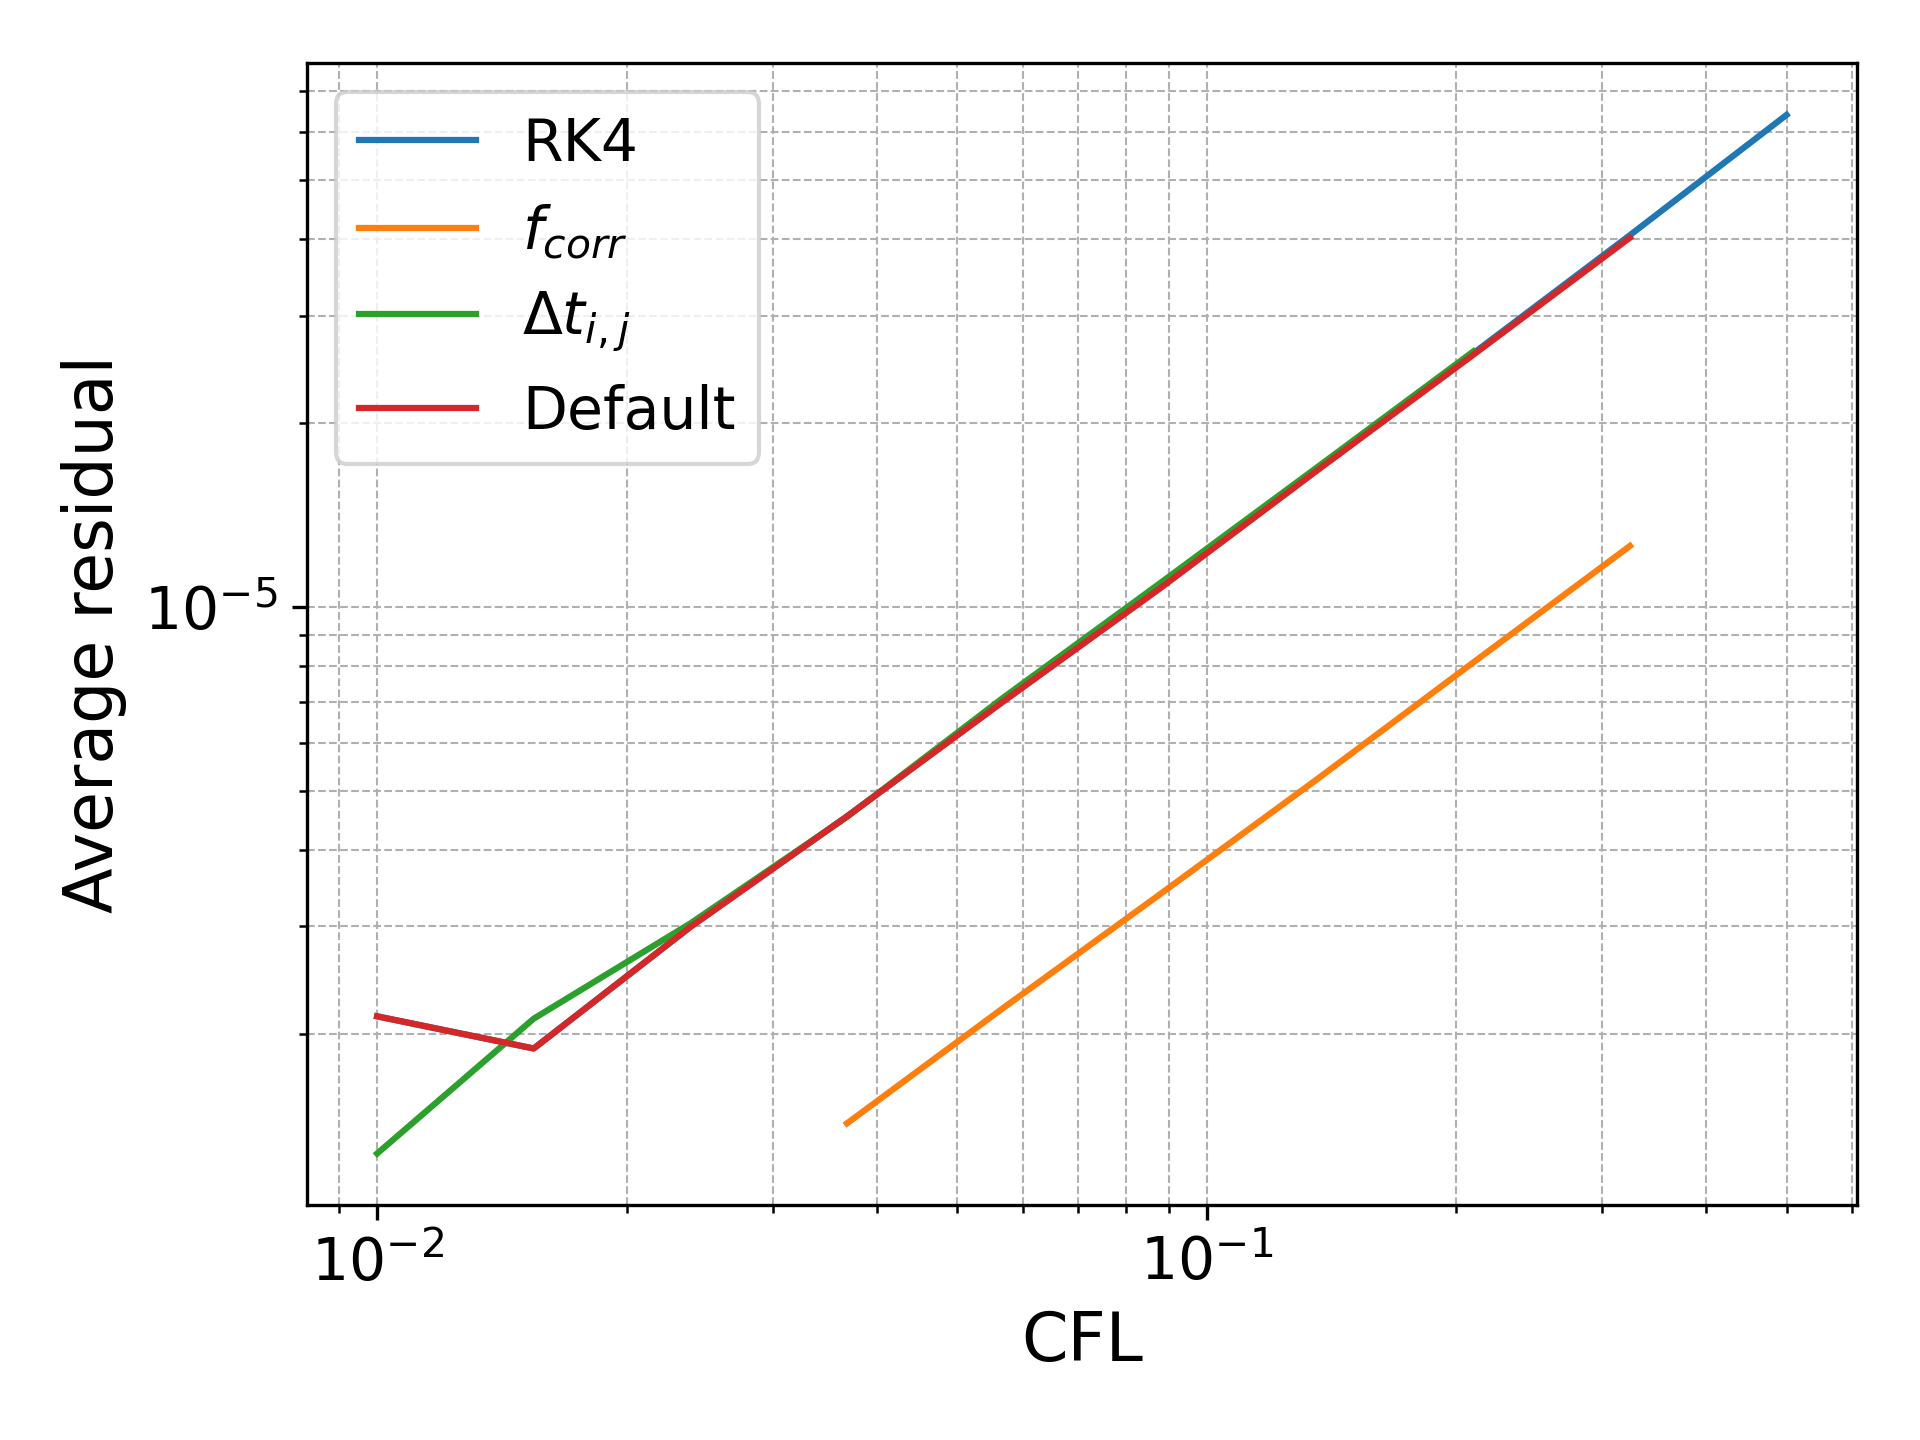
\includegraphics[width=0.99\textwidth]{figures/improvements_cfl_residual.png}
        \caption{Varying \texttt{cfl} with \texttt{ni} = 53}
        \label{fig:improvements_cfl_residual}
    \end{subfigure}
    \begin{subfigure}{0.49\textwidth}
        \centering
        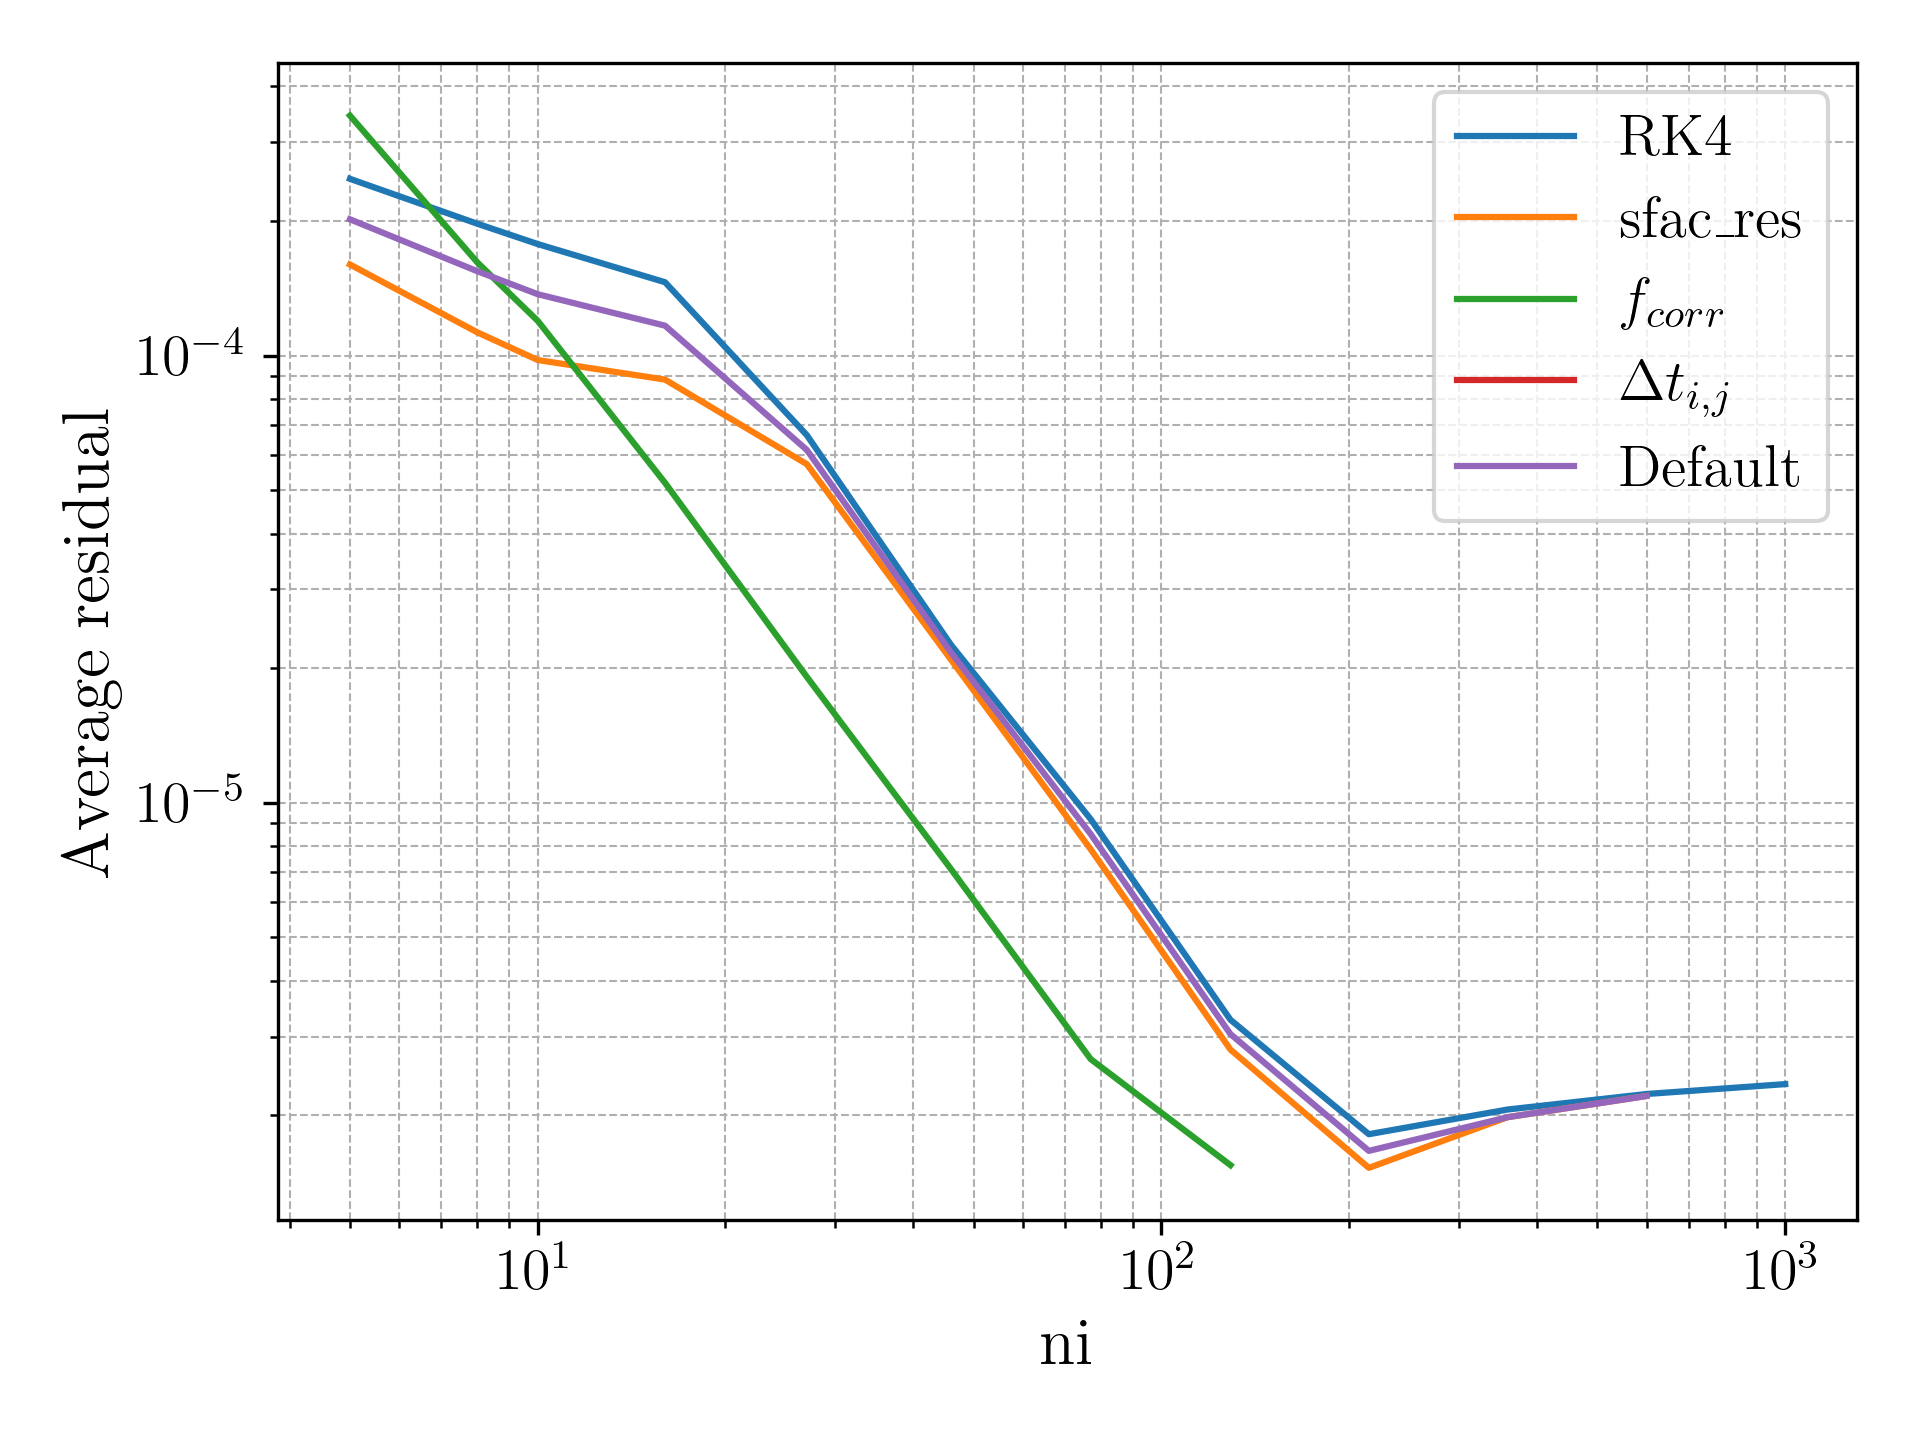
\includegraphics[width=0.99\textwidth]{figures/improvements_ni_residual.png}
        \caption{Varying \texttt{ni} with \texttt{cfl} = 0.2}
        \label{fig:improvements_ni_residual}
    \end{subfigure}
    \caption{Spatial and temporal accuracy of improvements}
\end{figure}

\begin{figure}[H]
    \centering
    \begin{subfigure}{0.49\textwidth}
        \centering
        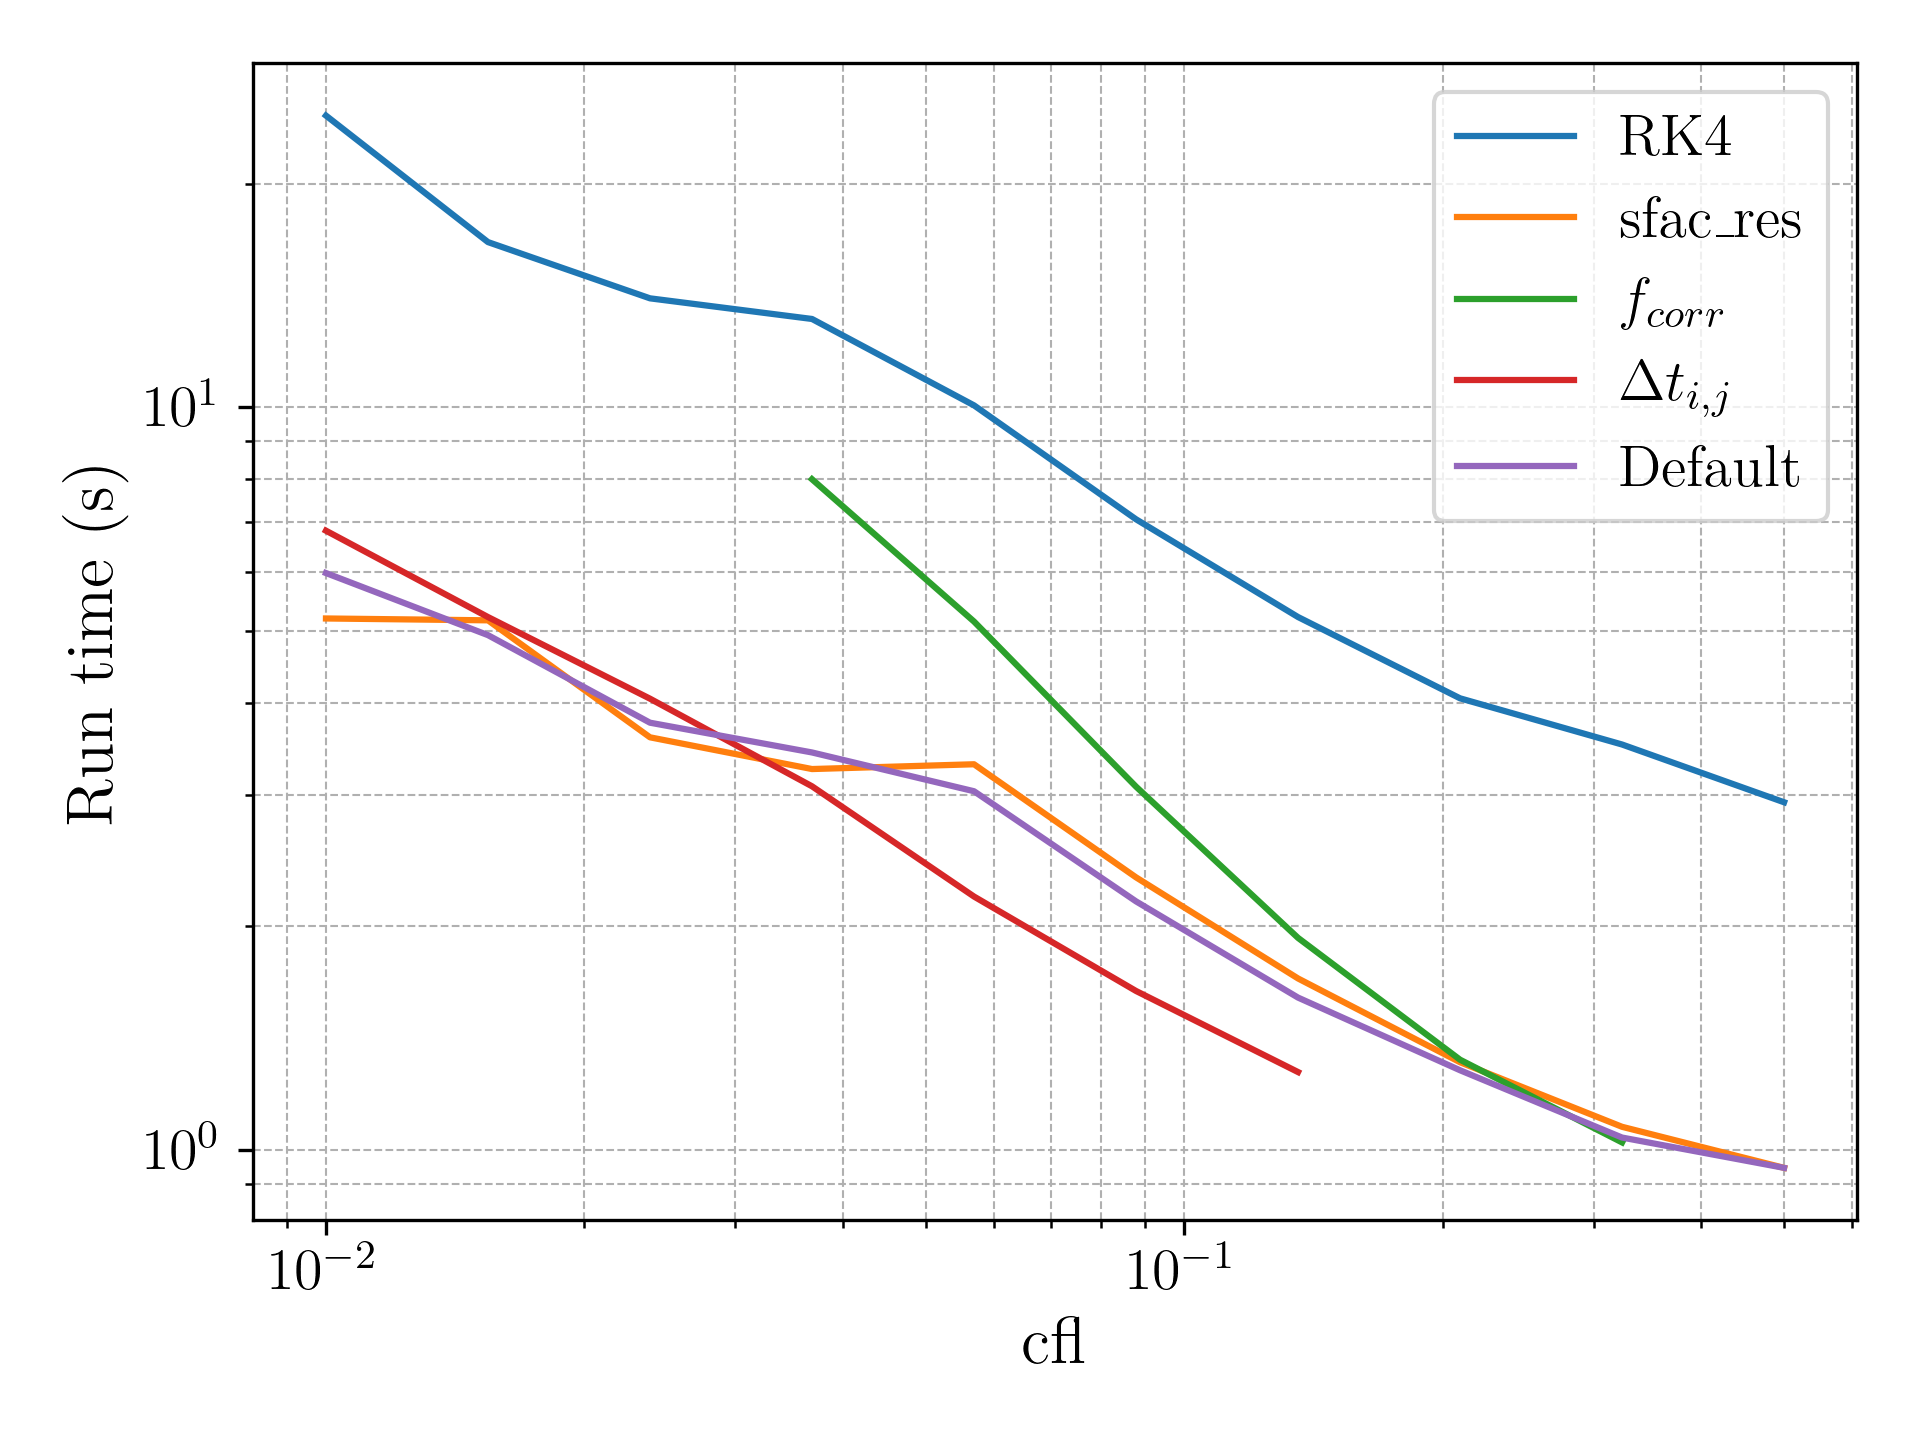
\includegraphics[width=0.99\textwidth]{figures/improvements_cfl_time.png}
        \caption{Varying CFL number}
        \label{fig:improvements_cfl_time}
    \end{subfigure}
    \begin{subfigure}{0.49\textwidth}
        \centering
        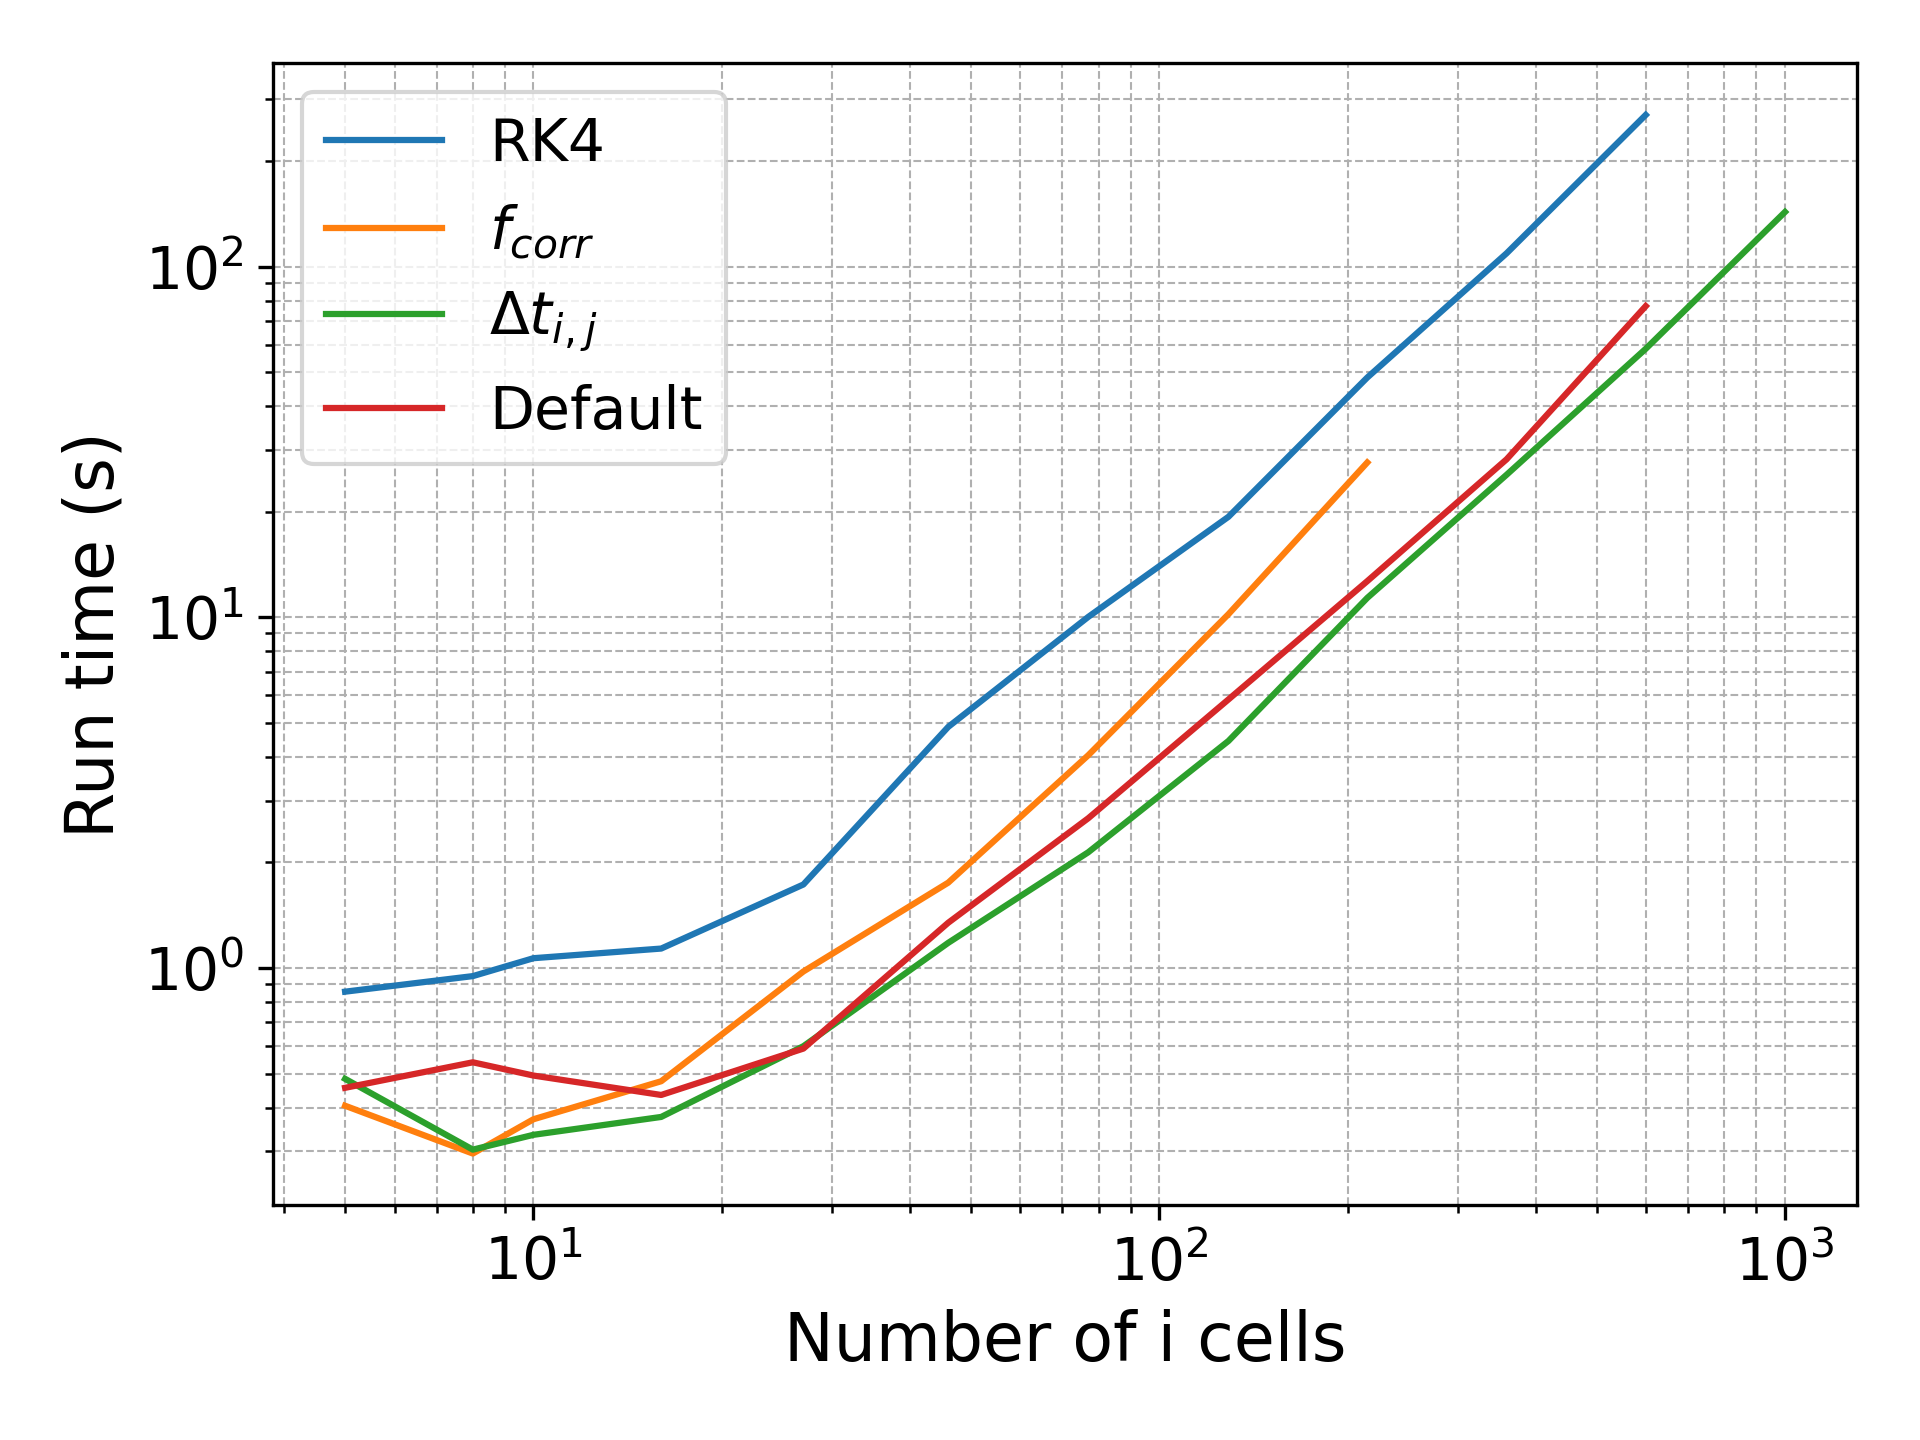
\includegraphics[width=0.99\textwidth]{figures/improvements_ni_time.png}
        \caption{Varying number of cells in \texttt{i} direction}
        \label{fig:improvements_ni_time}
    \end{subfigure}
    \caption{Spatial and temporal impact on runtime}
\end{figure}

\begin{figure}[H]
    \centering
    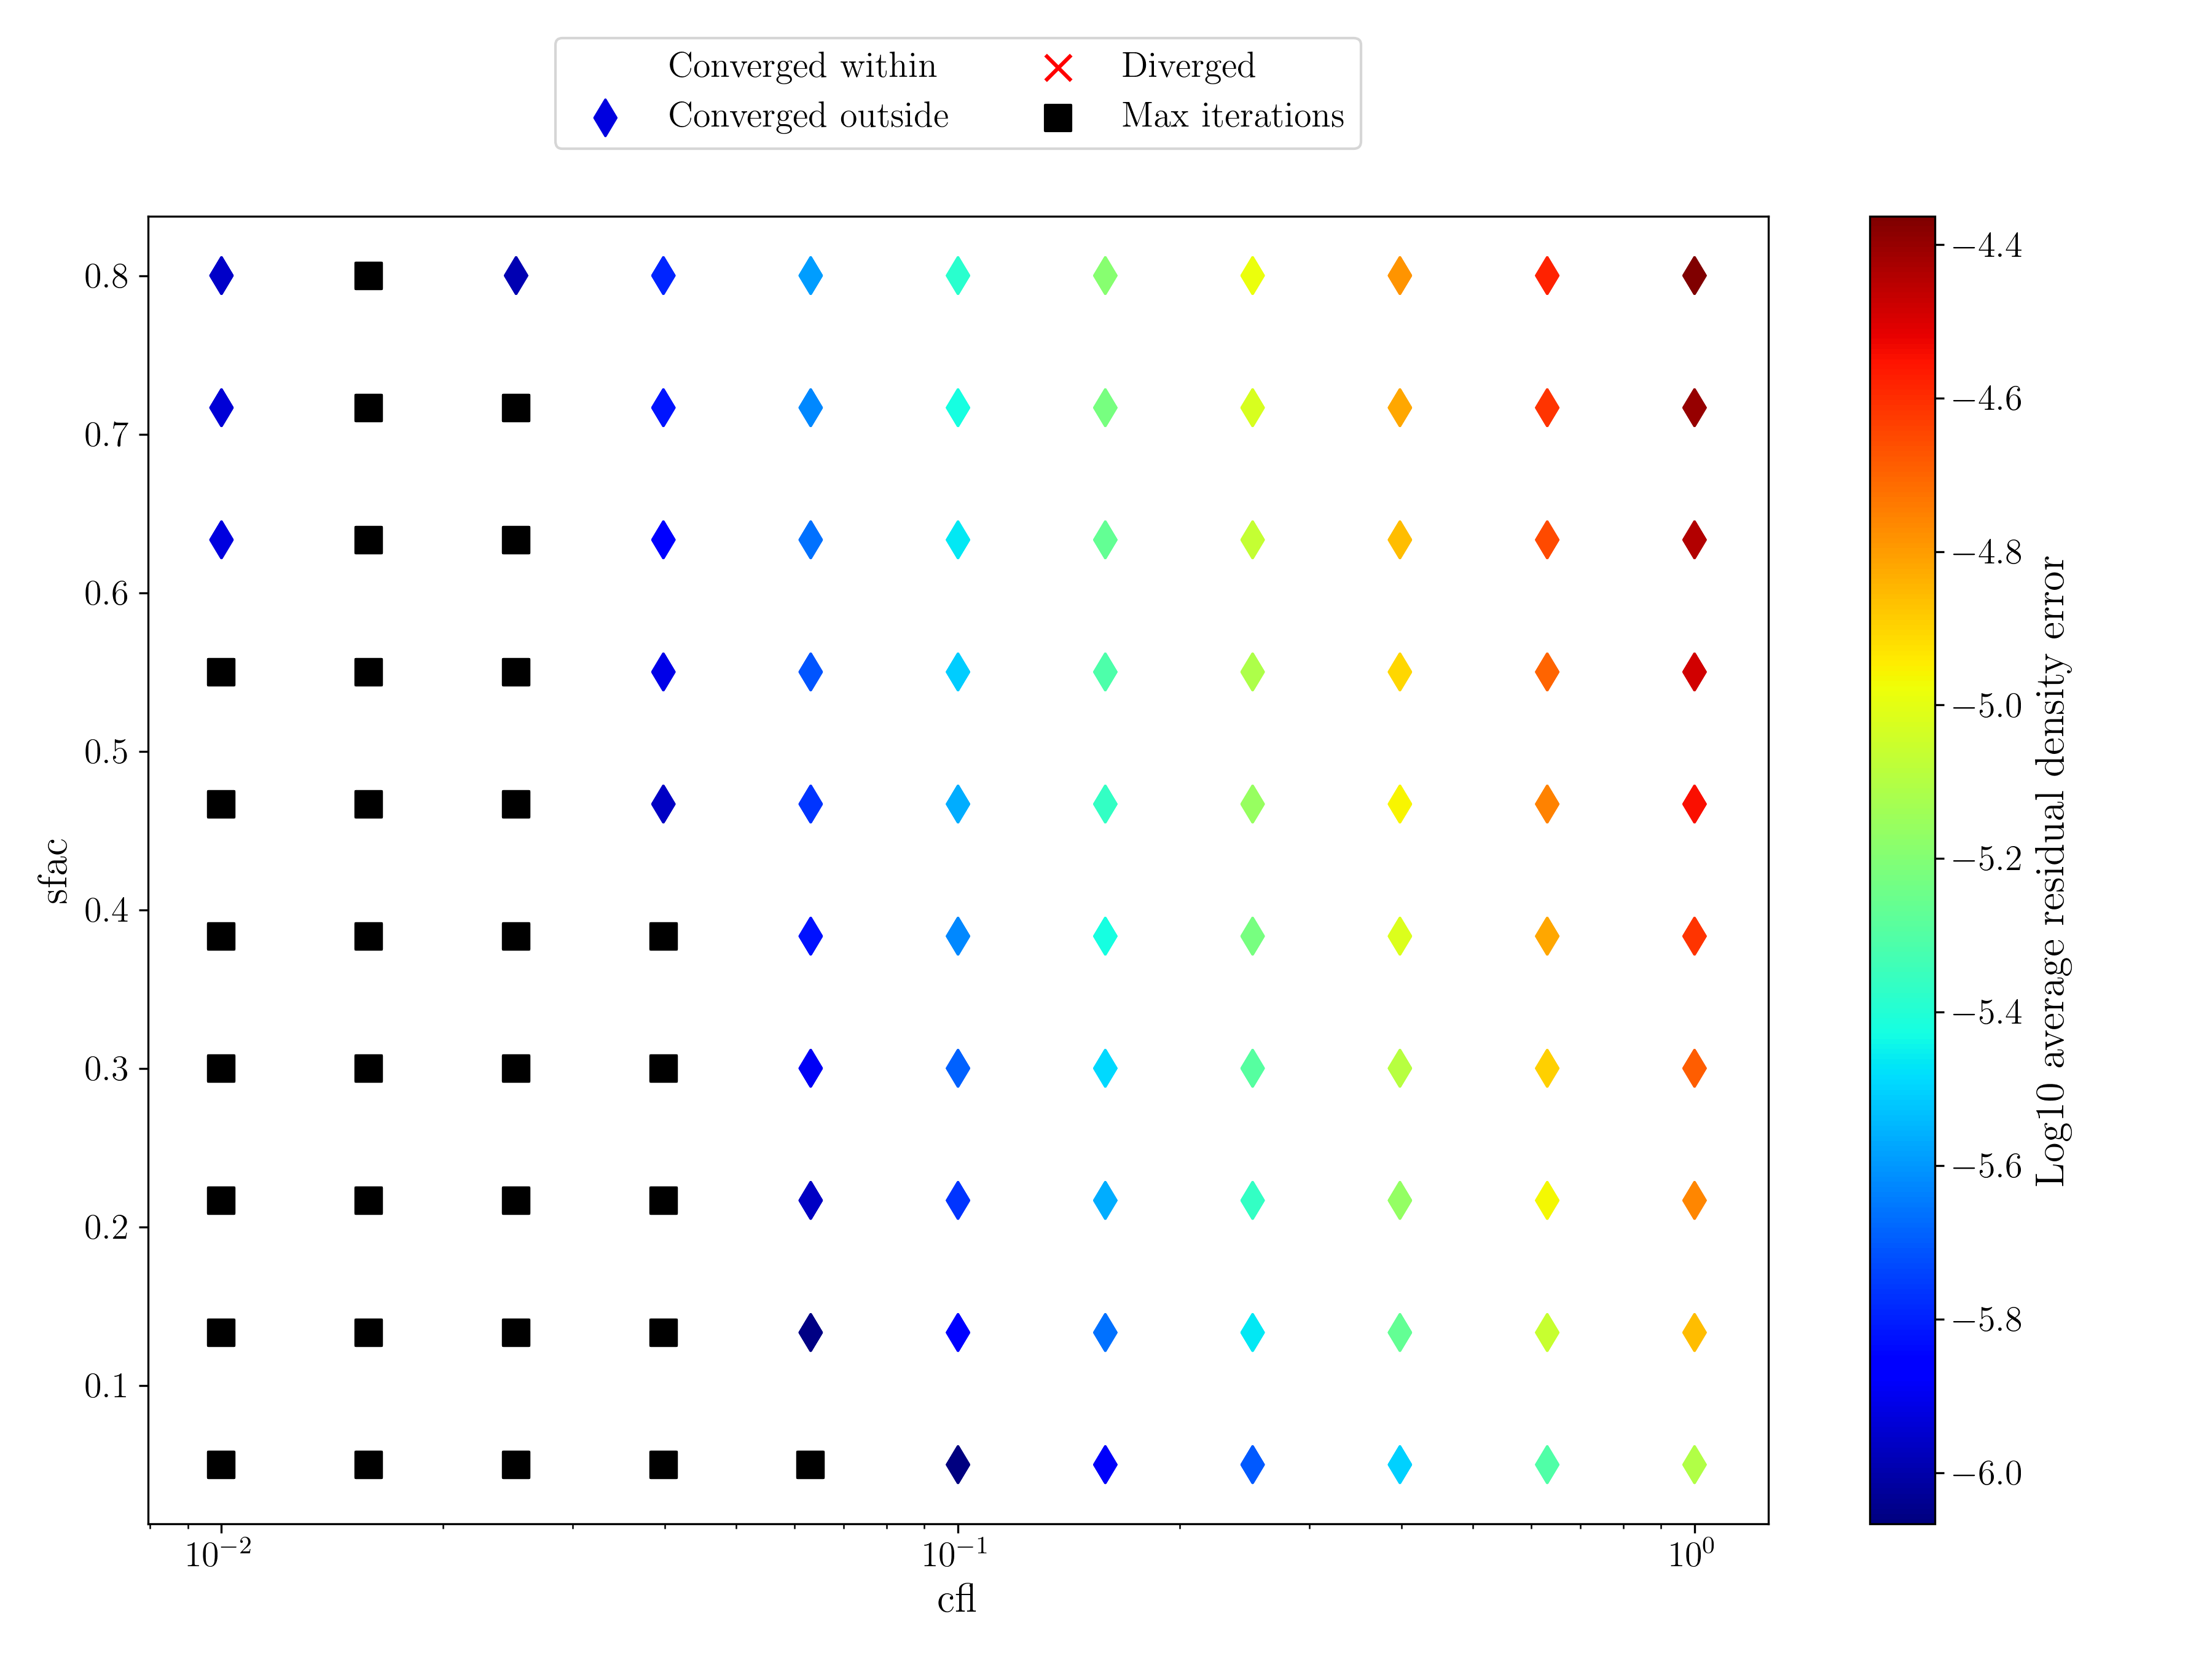
\includegraphics[width=0.7\textwidth]{figures/cfl_sfac_dro_avg.png}
    \caption{}
    \label{fig:cfl_sfac_dro_avg}
\end{figure}

\subsection{Effort vs Accuracy}

\begin{figure}[H]
    \begin{subfigure}{0.49\textwidth}
        \centering
        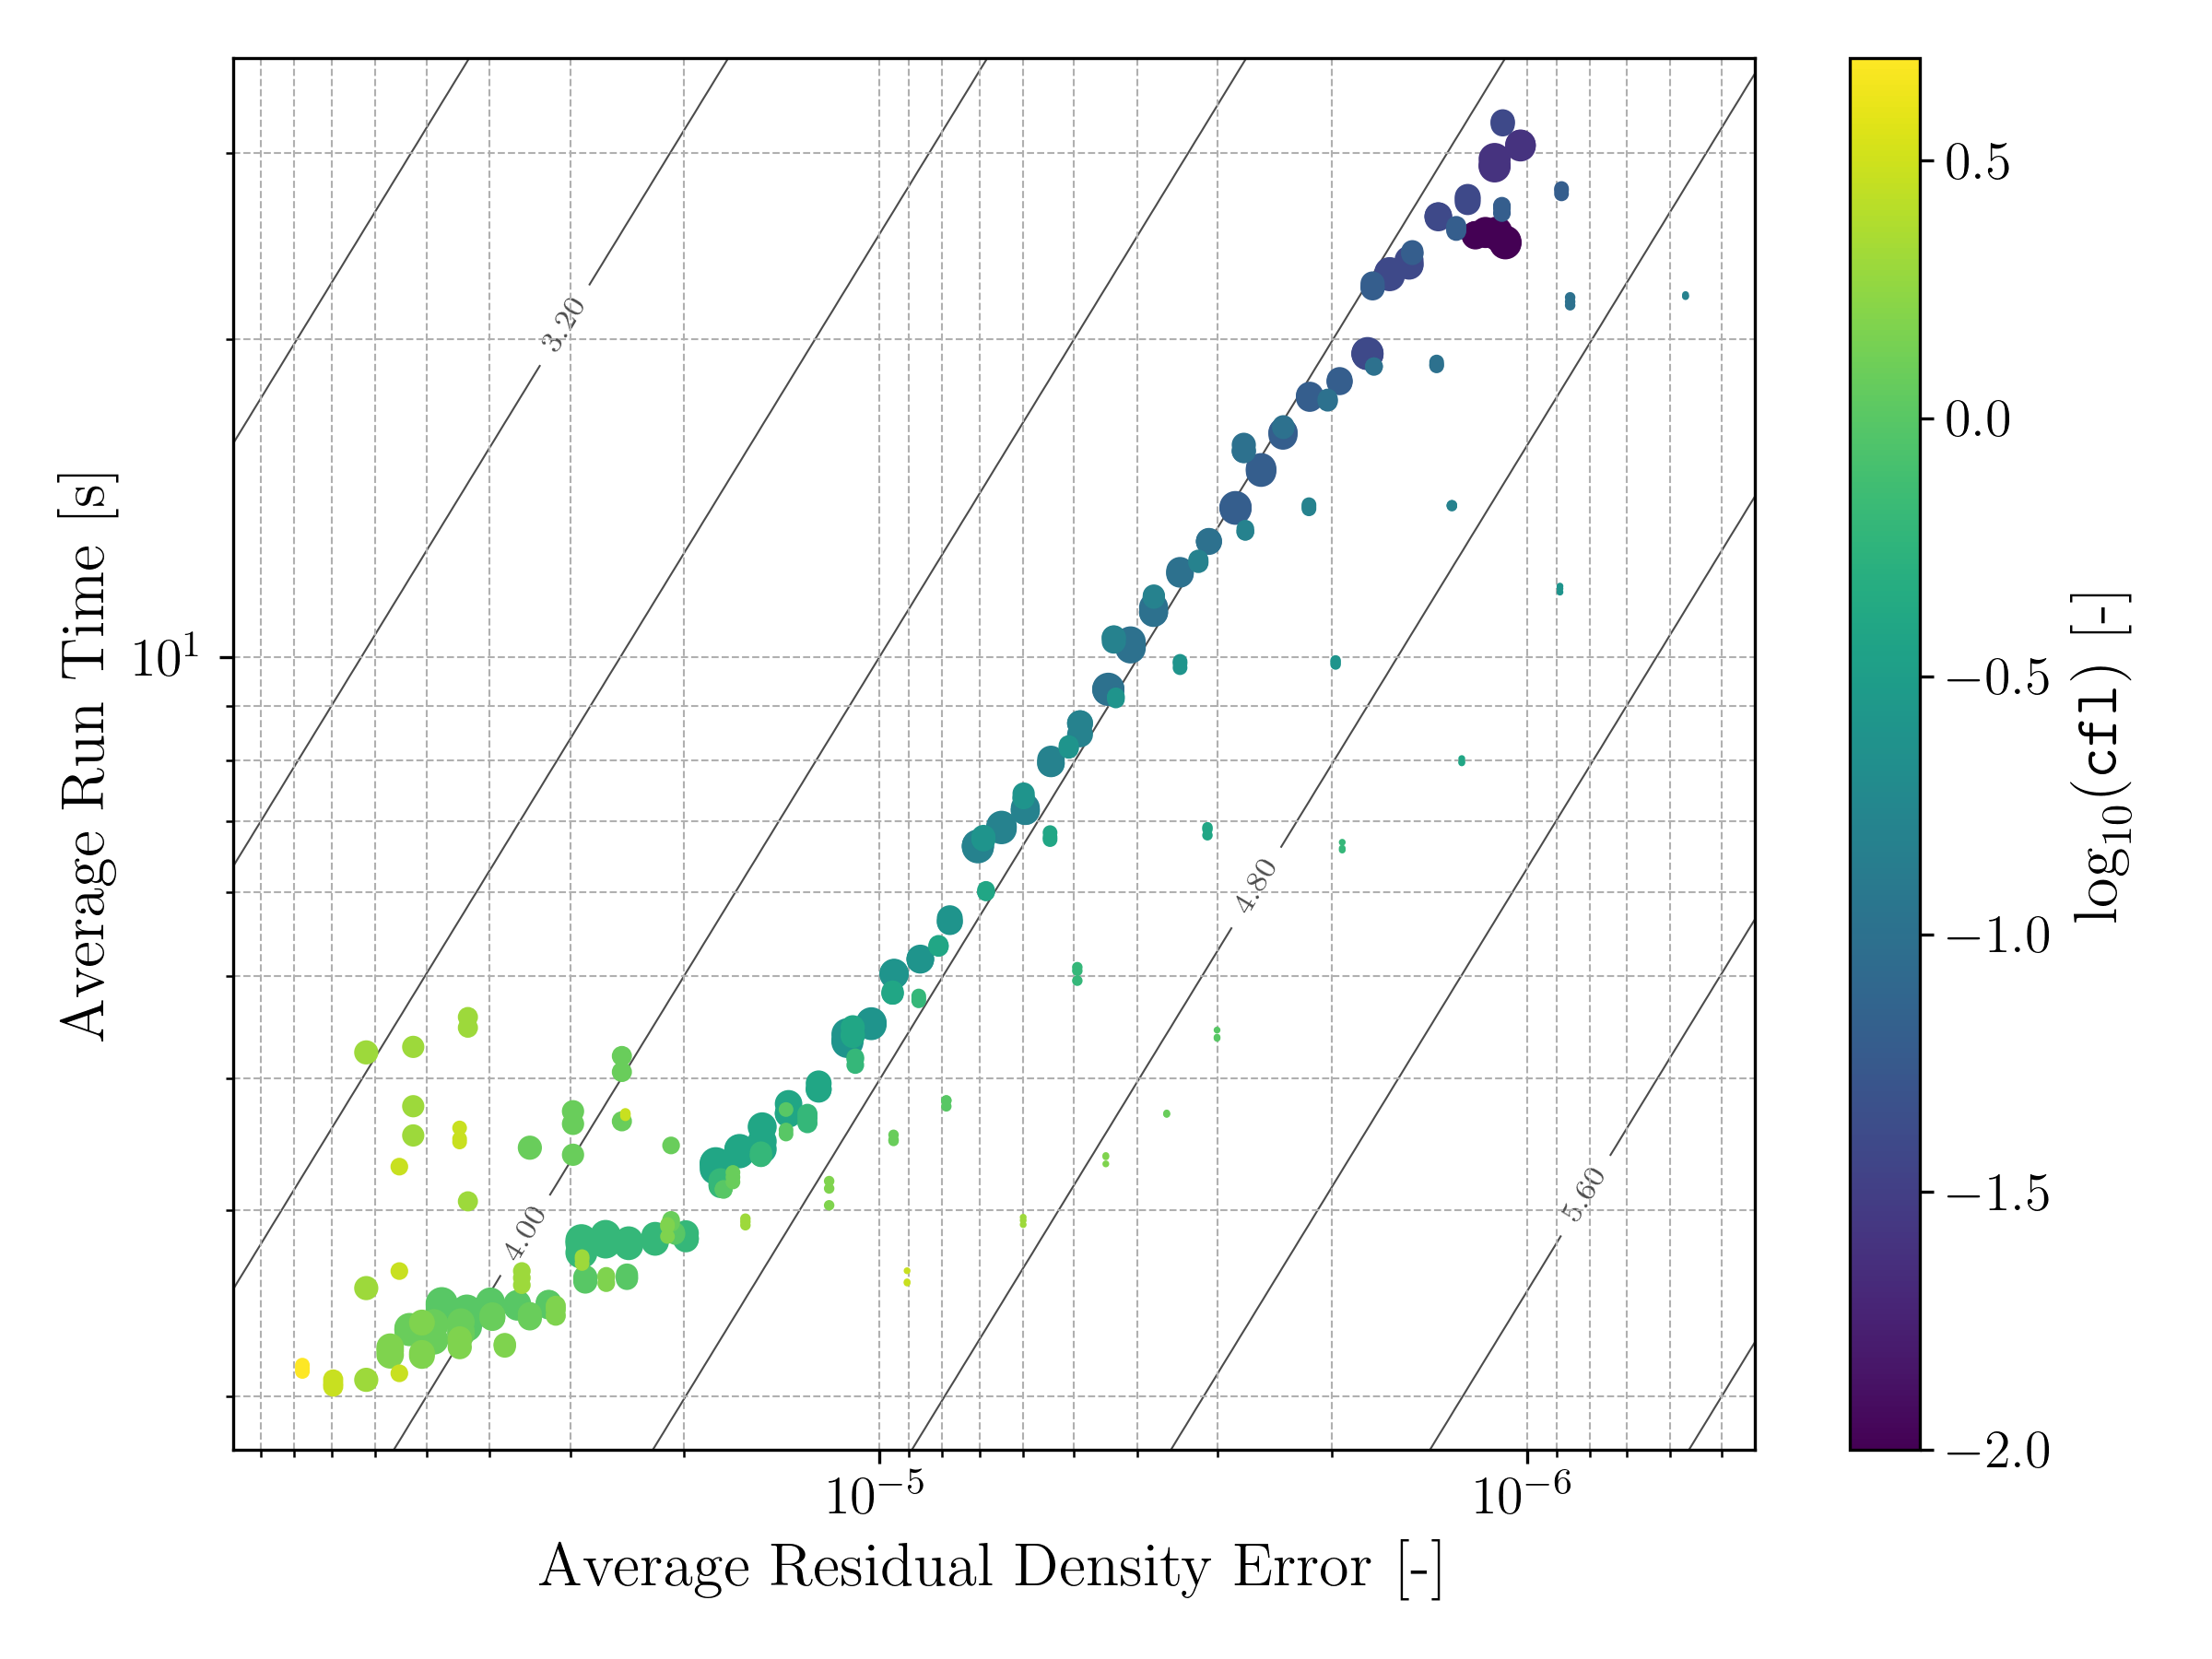
\includegraphics[width=0.99\textwidth]{figures/effort_vs_accuracy_cfl.png}
        \caption{Colour is $\log_{10}( \texttt{cfl})$ and size represents \\ $\texttt{sfac} \in [0.05, 0.8]$.}
        \label{fig:effort_vs_accuracy_cfl}
    \end{subfigure}
    \begin{subfigure}{0.49\textwidth}
        \centering
        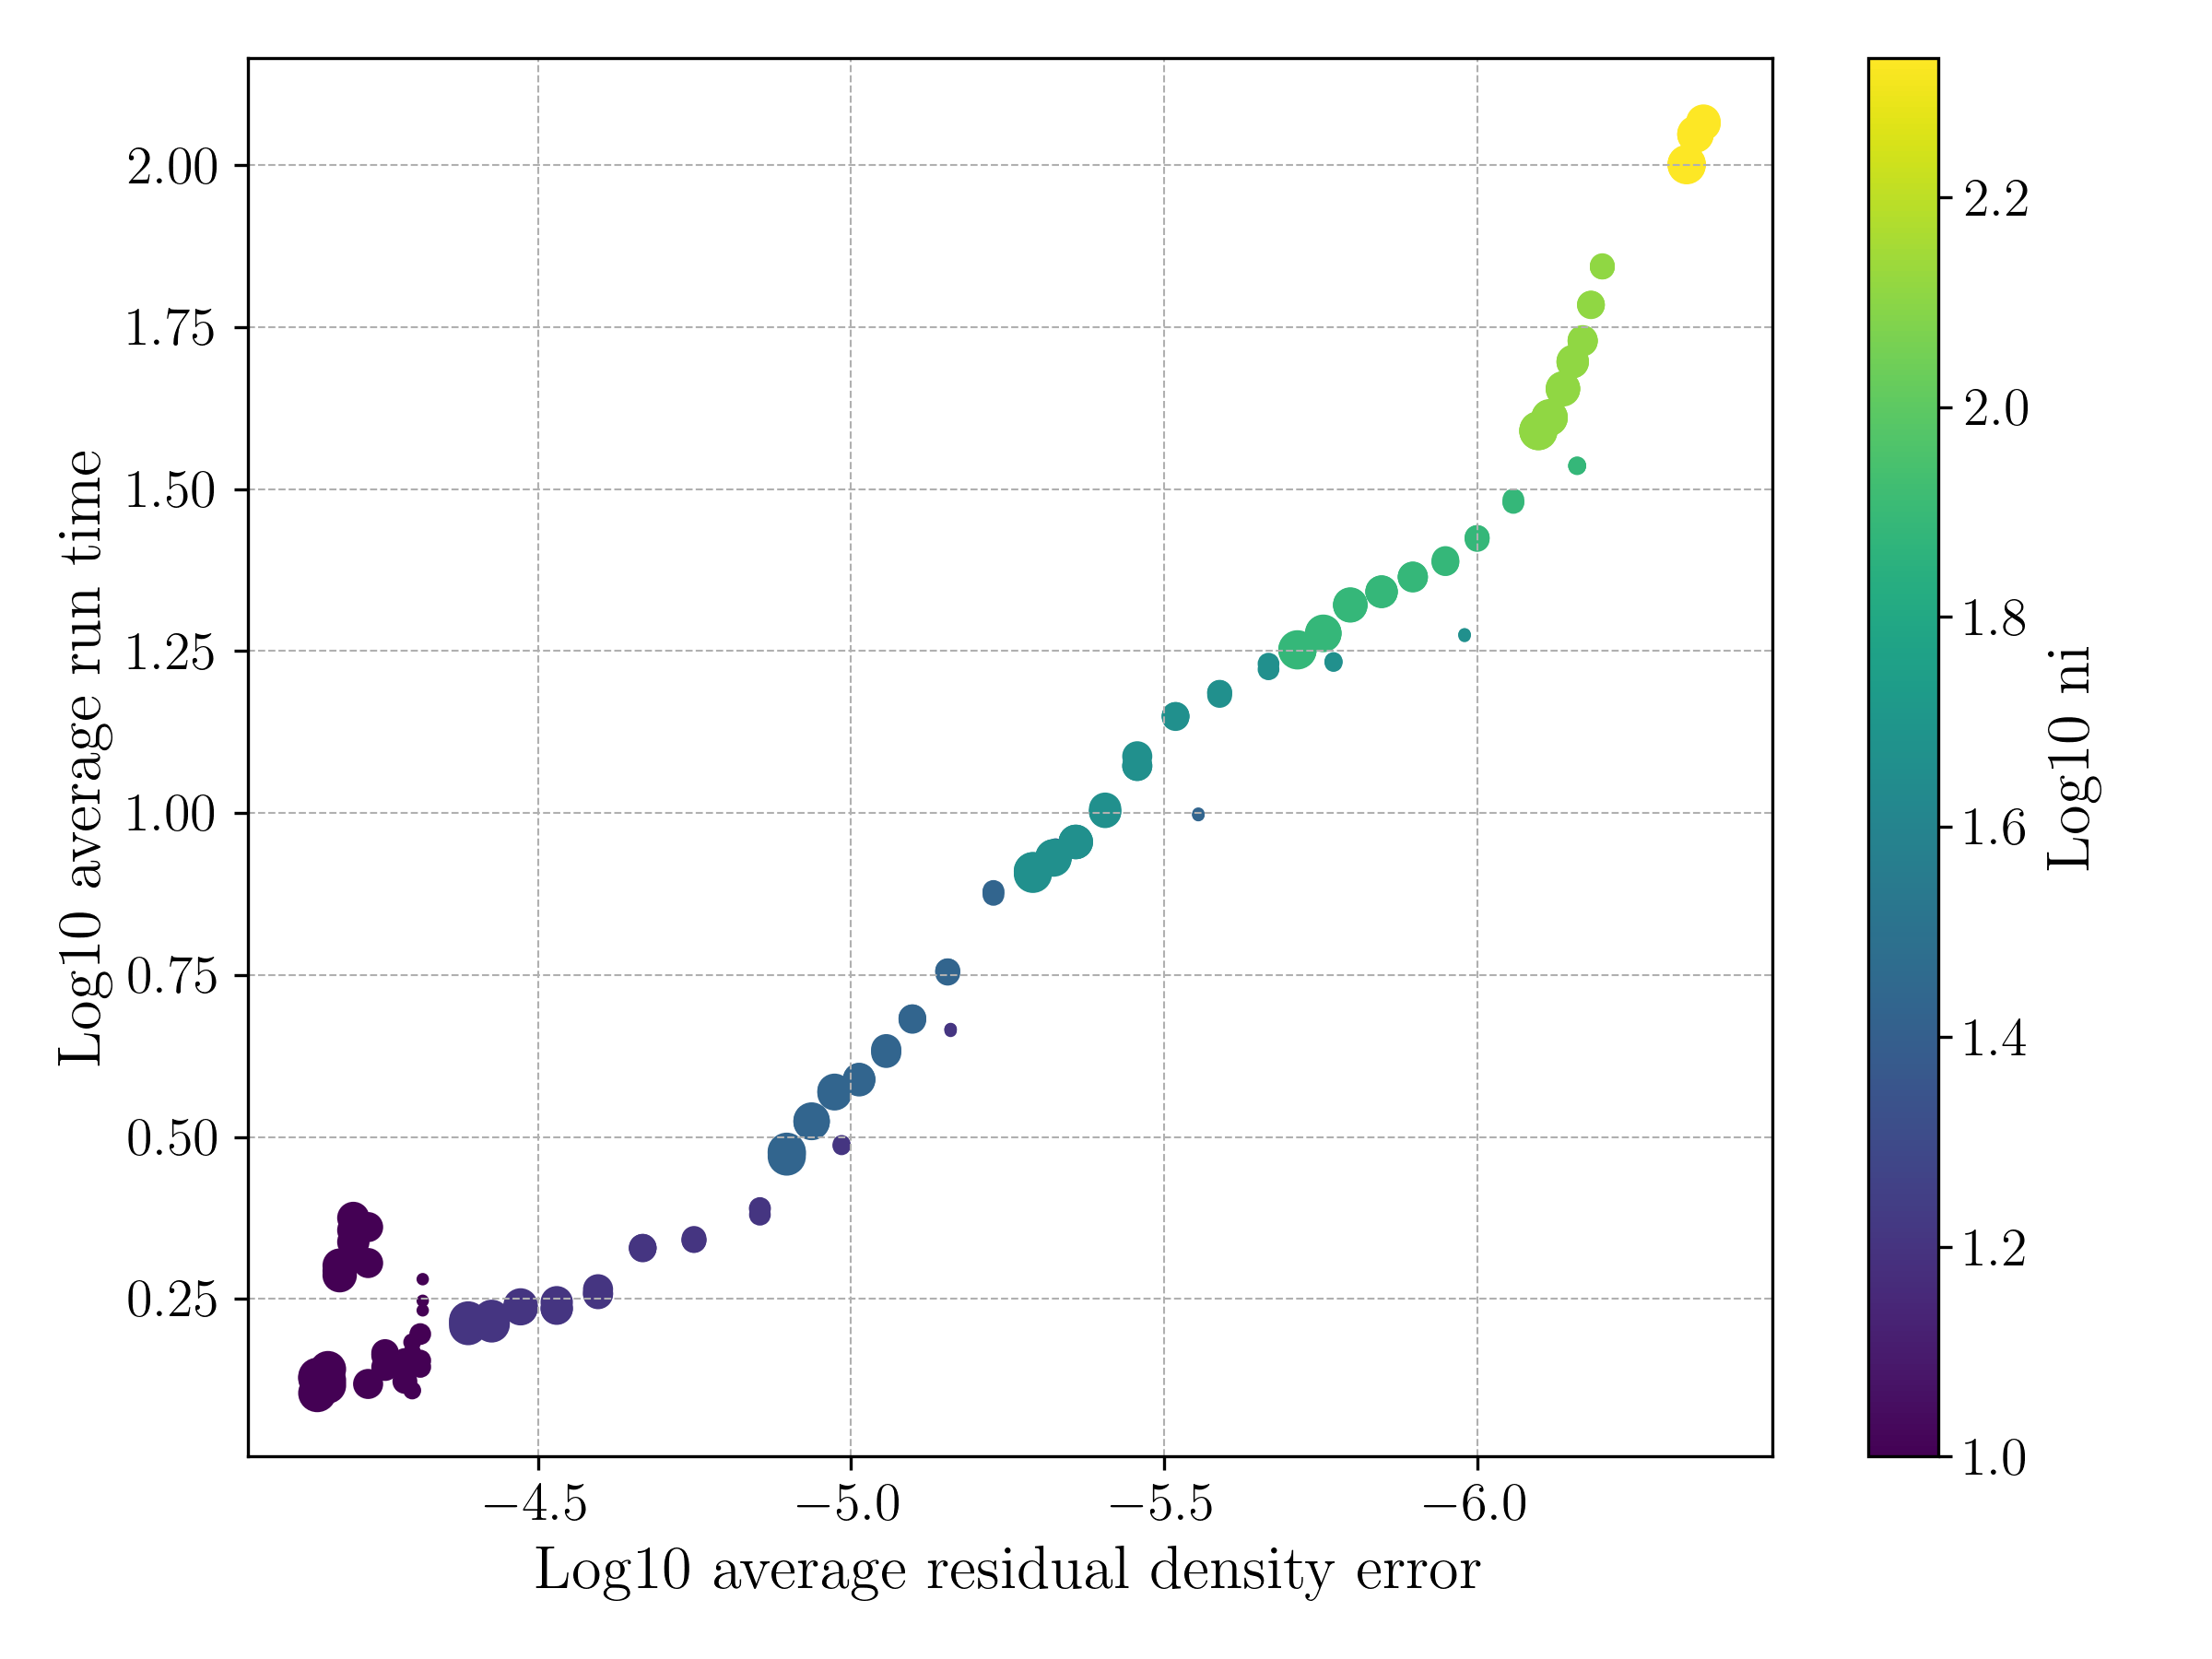
\includegraphics[width=0.99\textwidth]{figures/effort_vs_accuracy_ni.png}
        \caption{Colour is $\log_{10}( \texttt{ni})$ and size represents \\ $\texttt{sfac} \in [0.05, 0.8]$.}
        \label{fig:effort_vs_accuracy_ni}
    \end{subfigure}
    \caption{Effort vs accuracy for bump case with varying parameters. Contours are constant $FM$.}
    \label{fig:effort_vs_accuracy_1}
\end{figure}

\begin{figure}[H]
    \begin{subfigure}{0.49\textwidth}
        \centering
        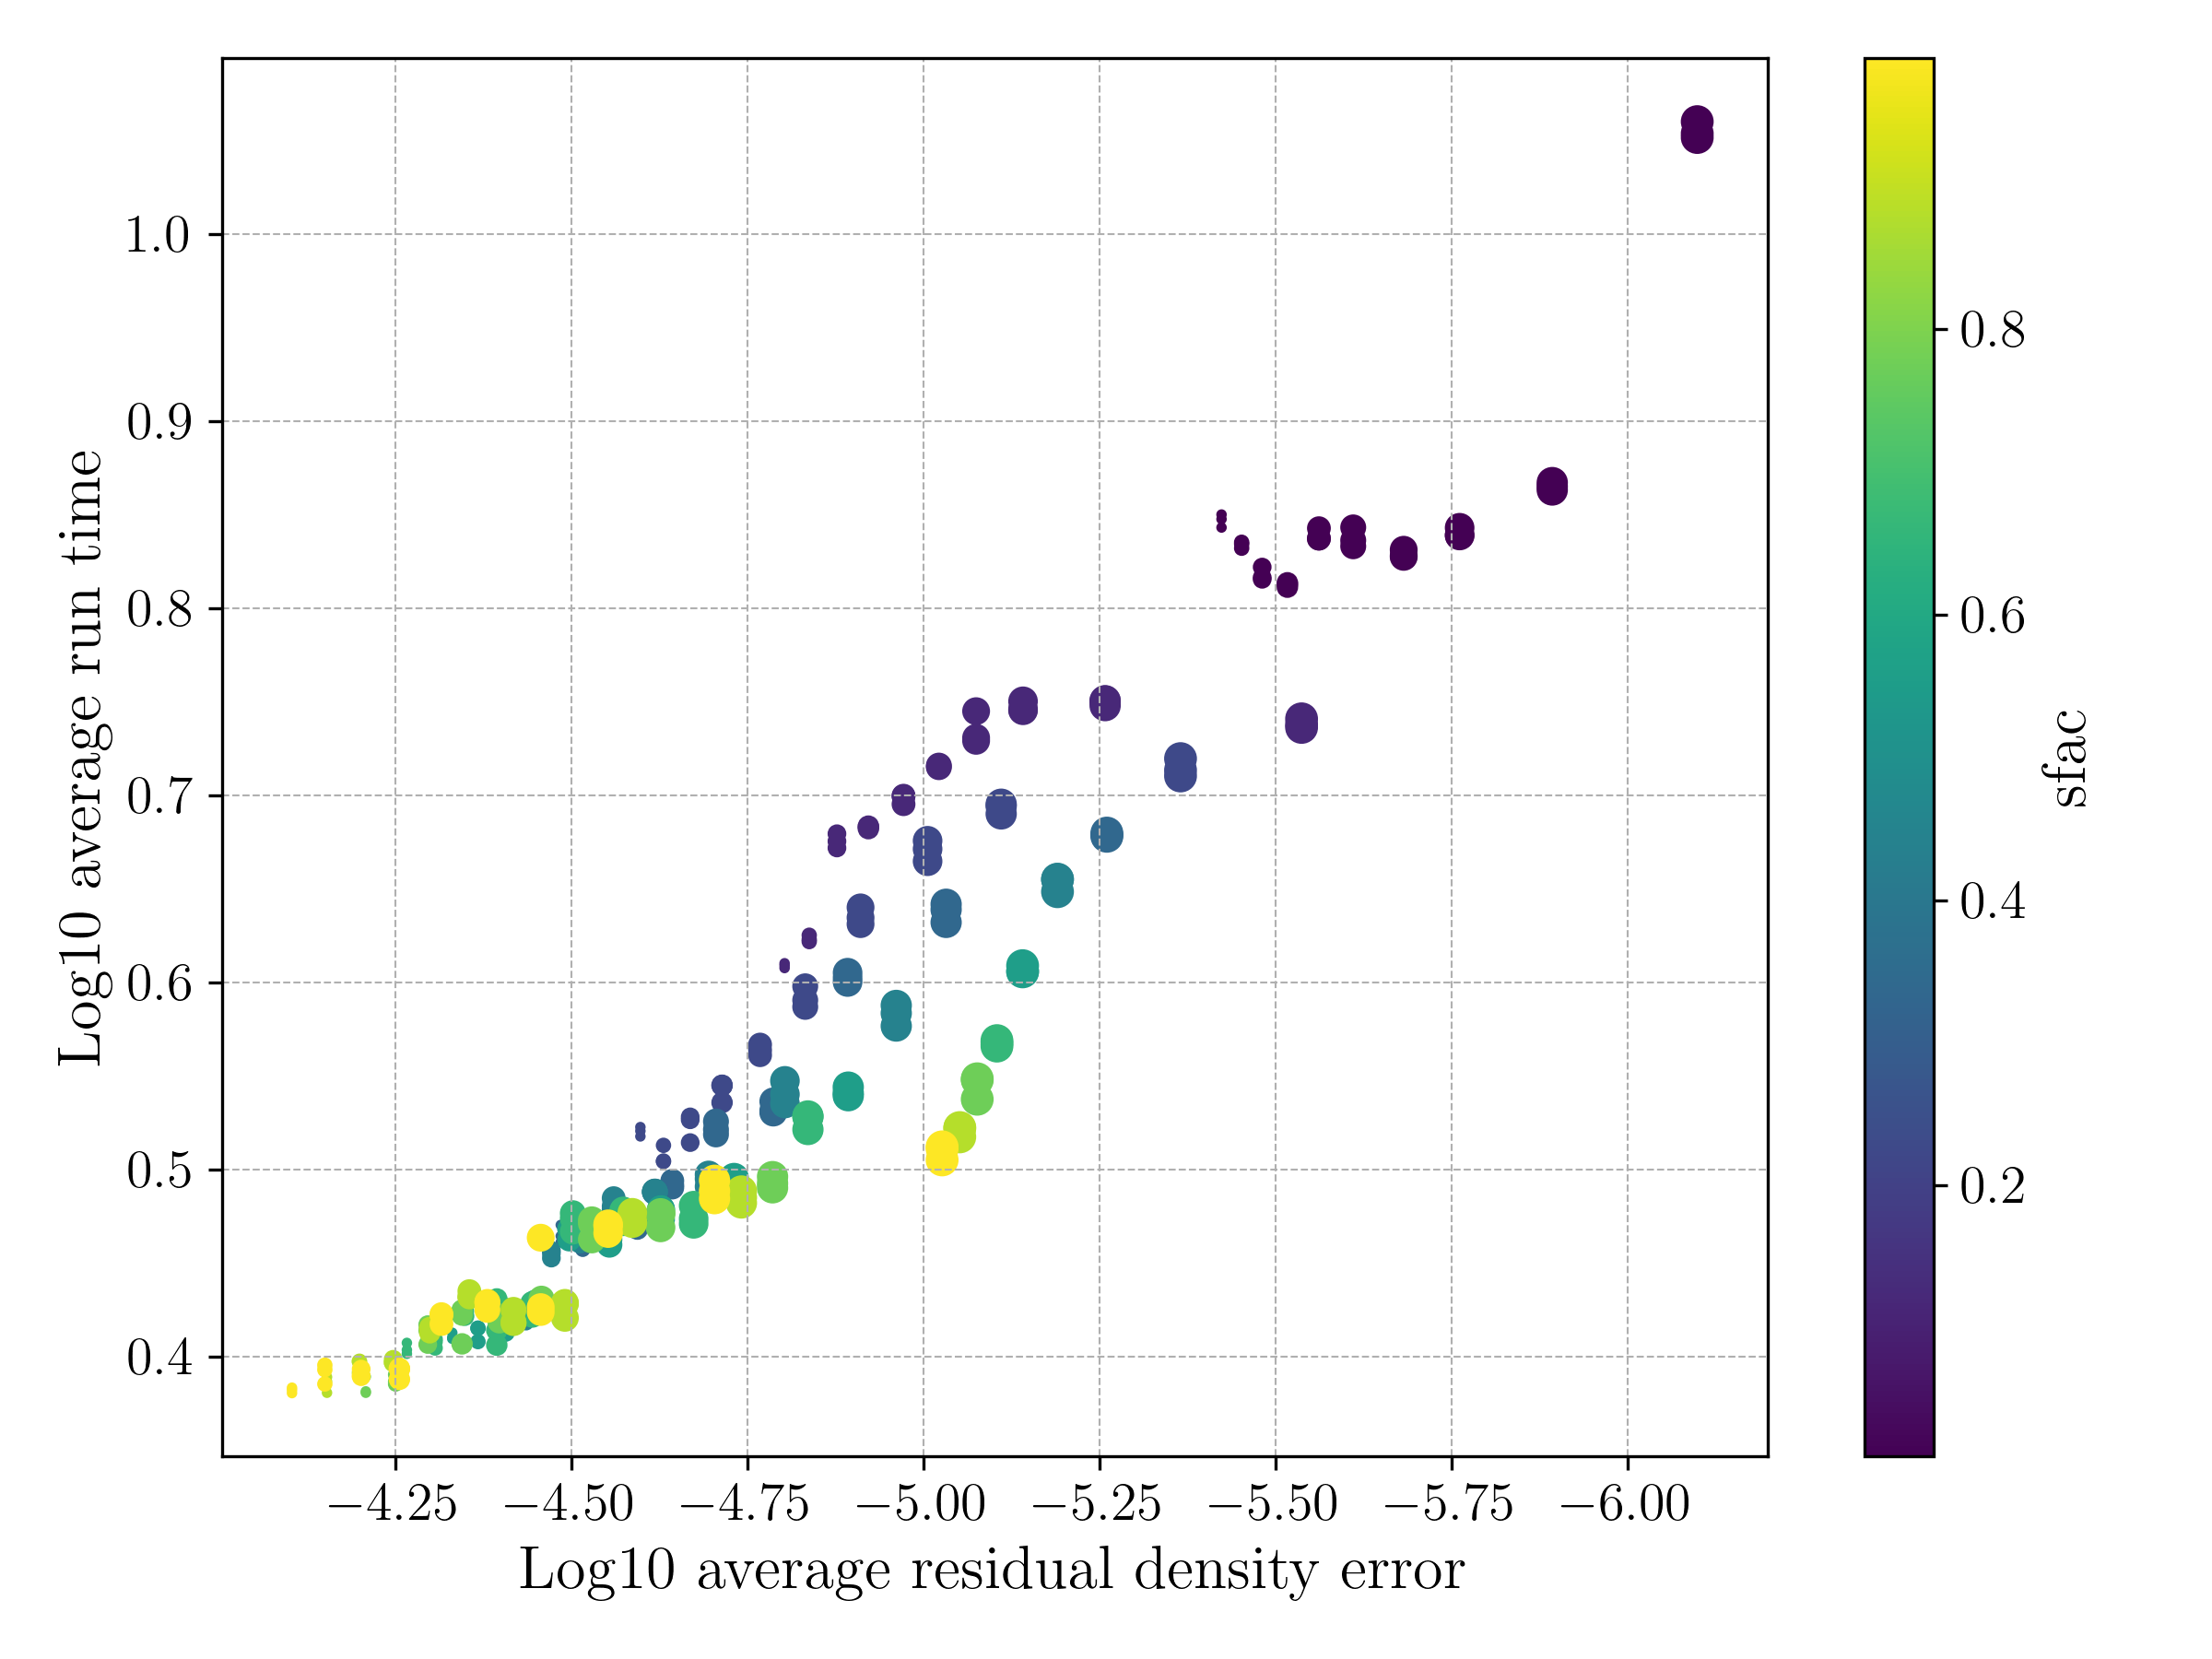
\includegraphics[width=0.99\textwidth]{figures/effort_vs_accuracy_fcorr.png}
        \caption{Colour is \texttt{sfac} and size represents \\ $\texttt{fcorr} \in [0.1, 0.9]$. }
        \label{fig:effort_vs_accuracy_fcorr}
    \end{subfigure}
    \begin{subfigure}{0.49\textwidth}
        \centering
        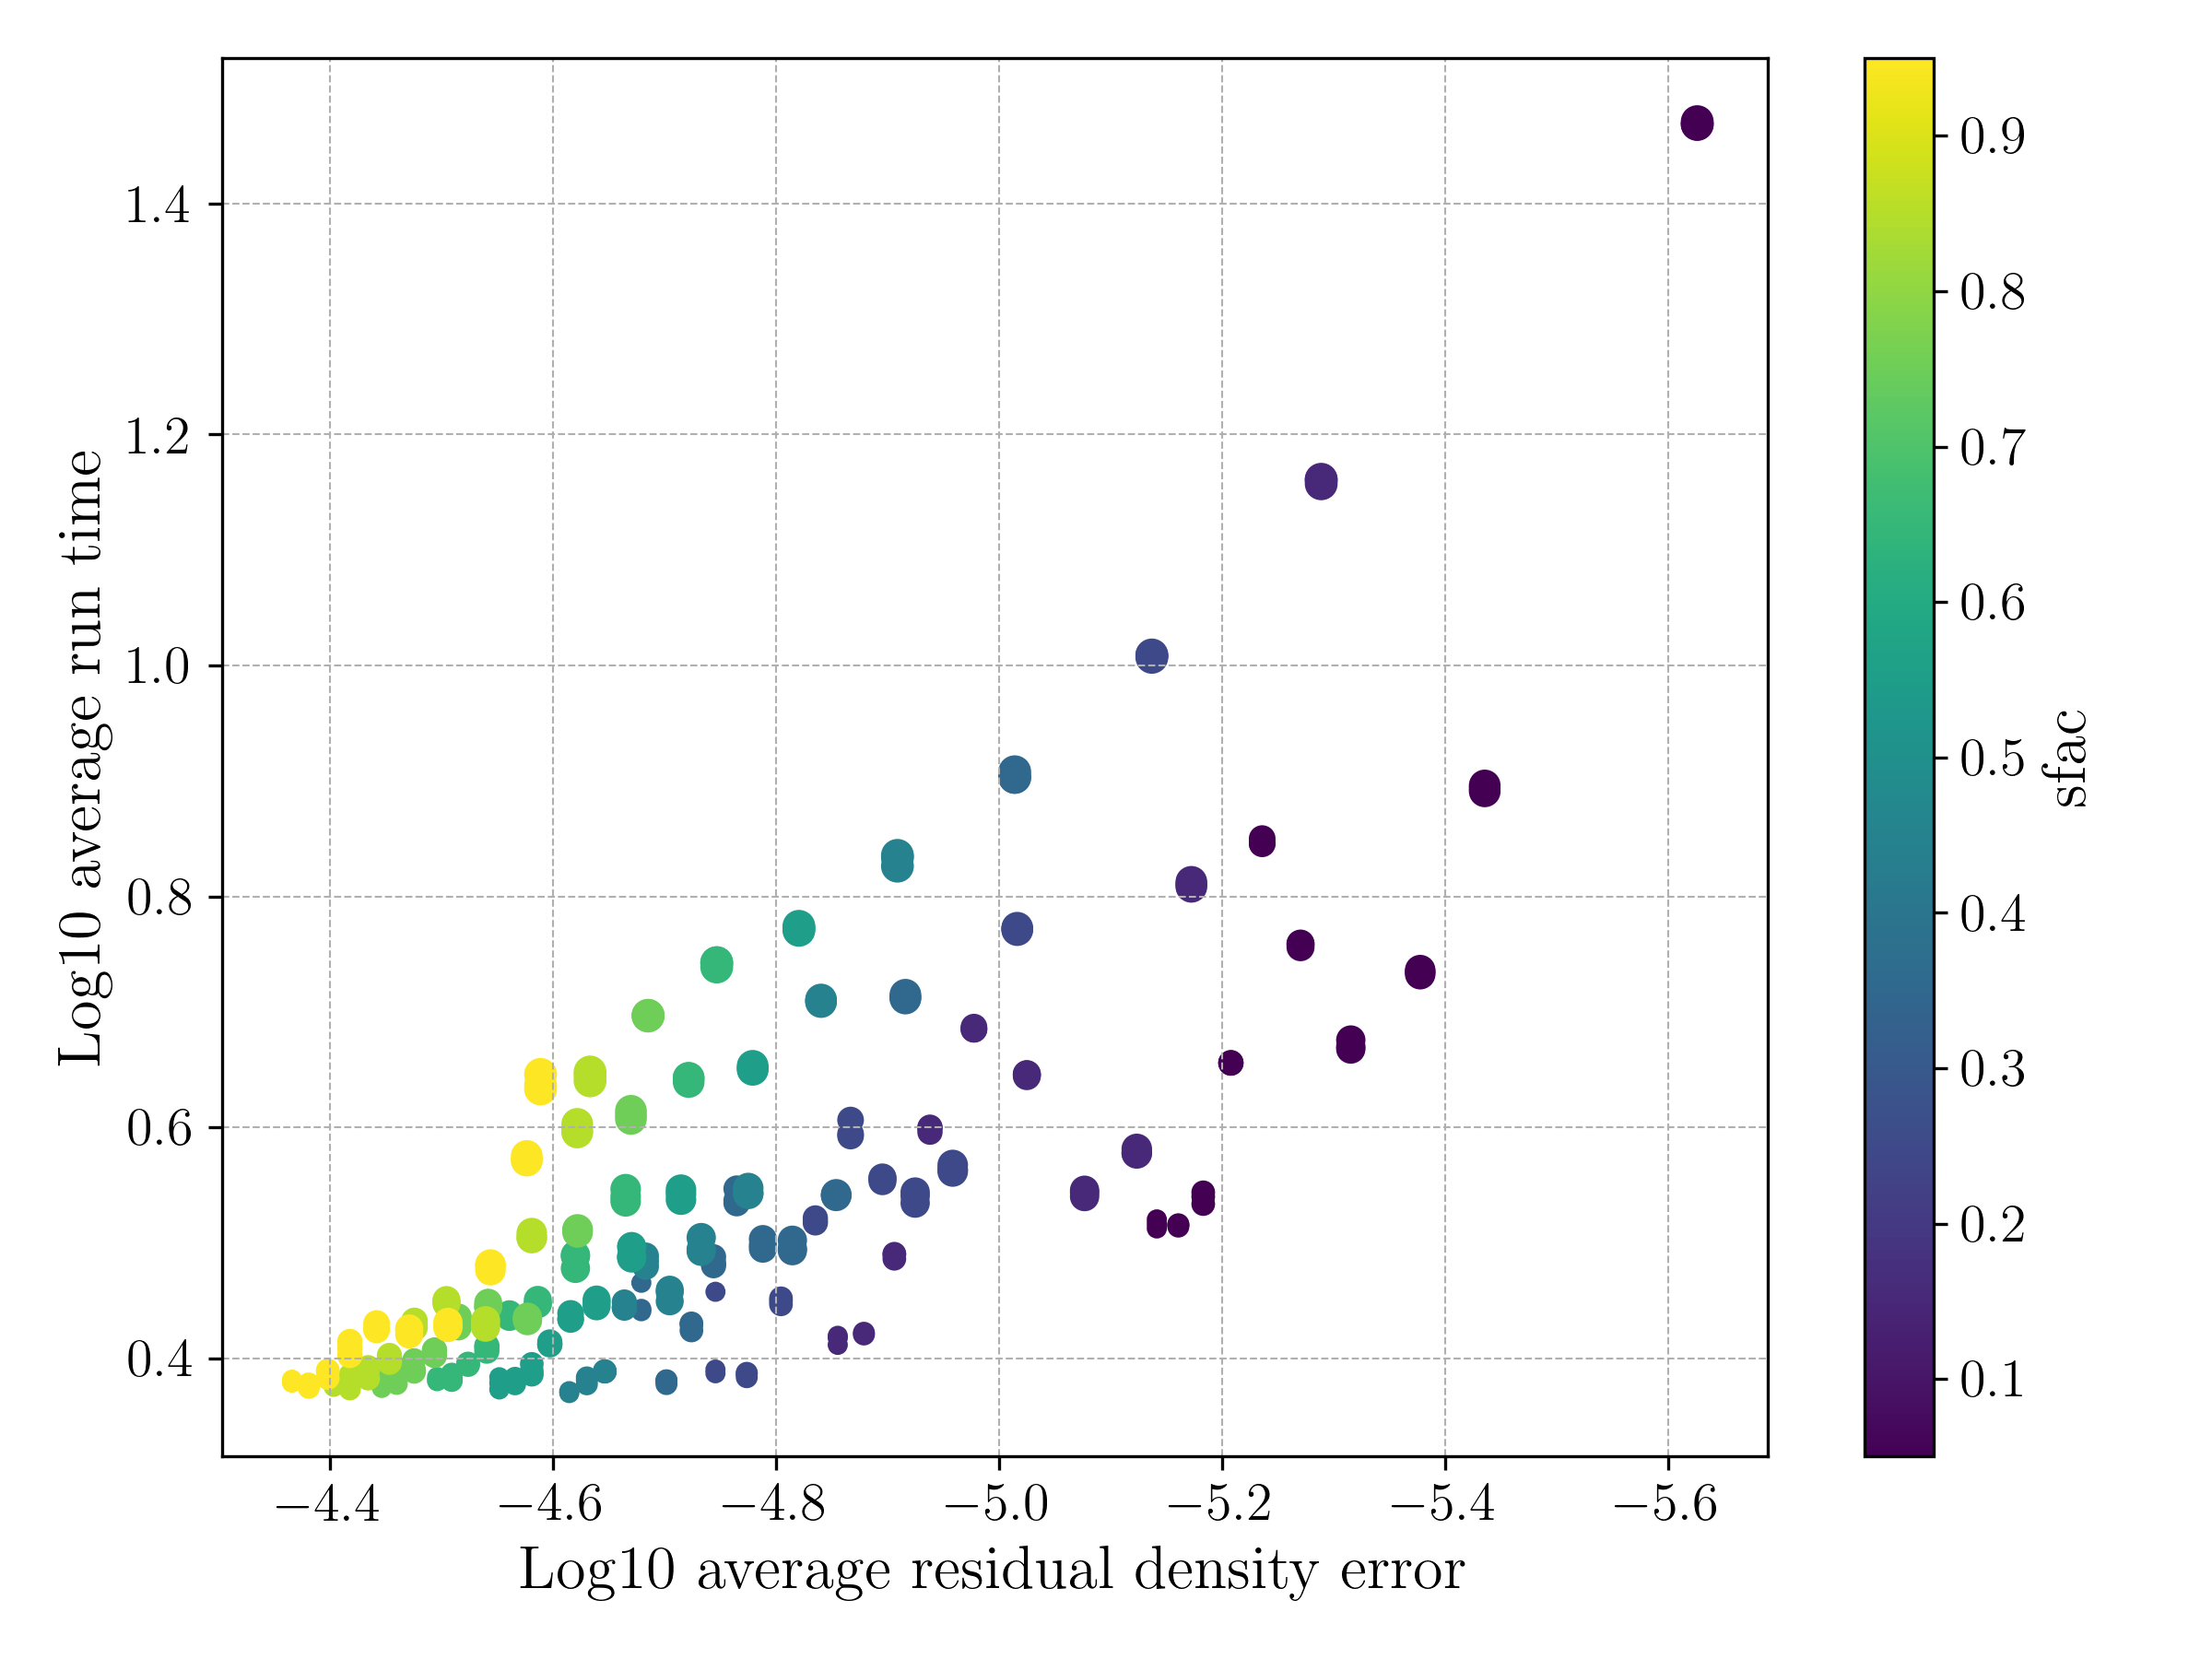
\includegraphics[width=0.99\textwidth]{figures/effort_vs_accuracy_sfac_res.png}
        \caption{Colour is $\log_{10}( \texttt{cfl})$ and size represents \\ $\texttt{sfac\_res} \in [0.1,0.95]$. \texttt{sfac} = 0.2}
        \label{fig:effort_vs_accuracy_sfac_res}
    \end{subfigure}
    \caption{Effort vs accuracy for bump case with varying parameters. Contours are constant $FM$.}
    \label{fig:effort_vs_accuracy_2}
\end{figure}

\subsection{NACA airfoils}

\begin{figure}[H]
    \centering
    \begin{subfigure}{0.49\textwidth}
        \centering
        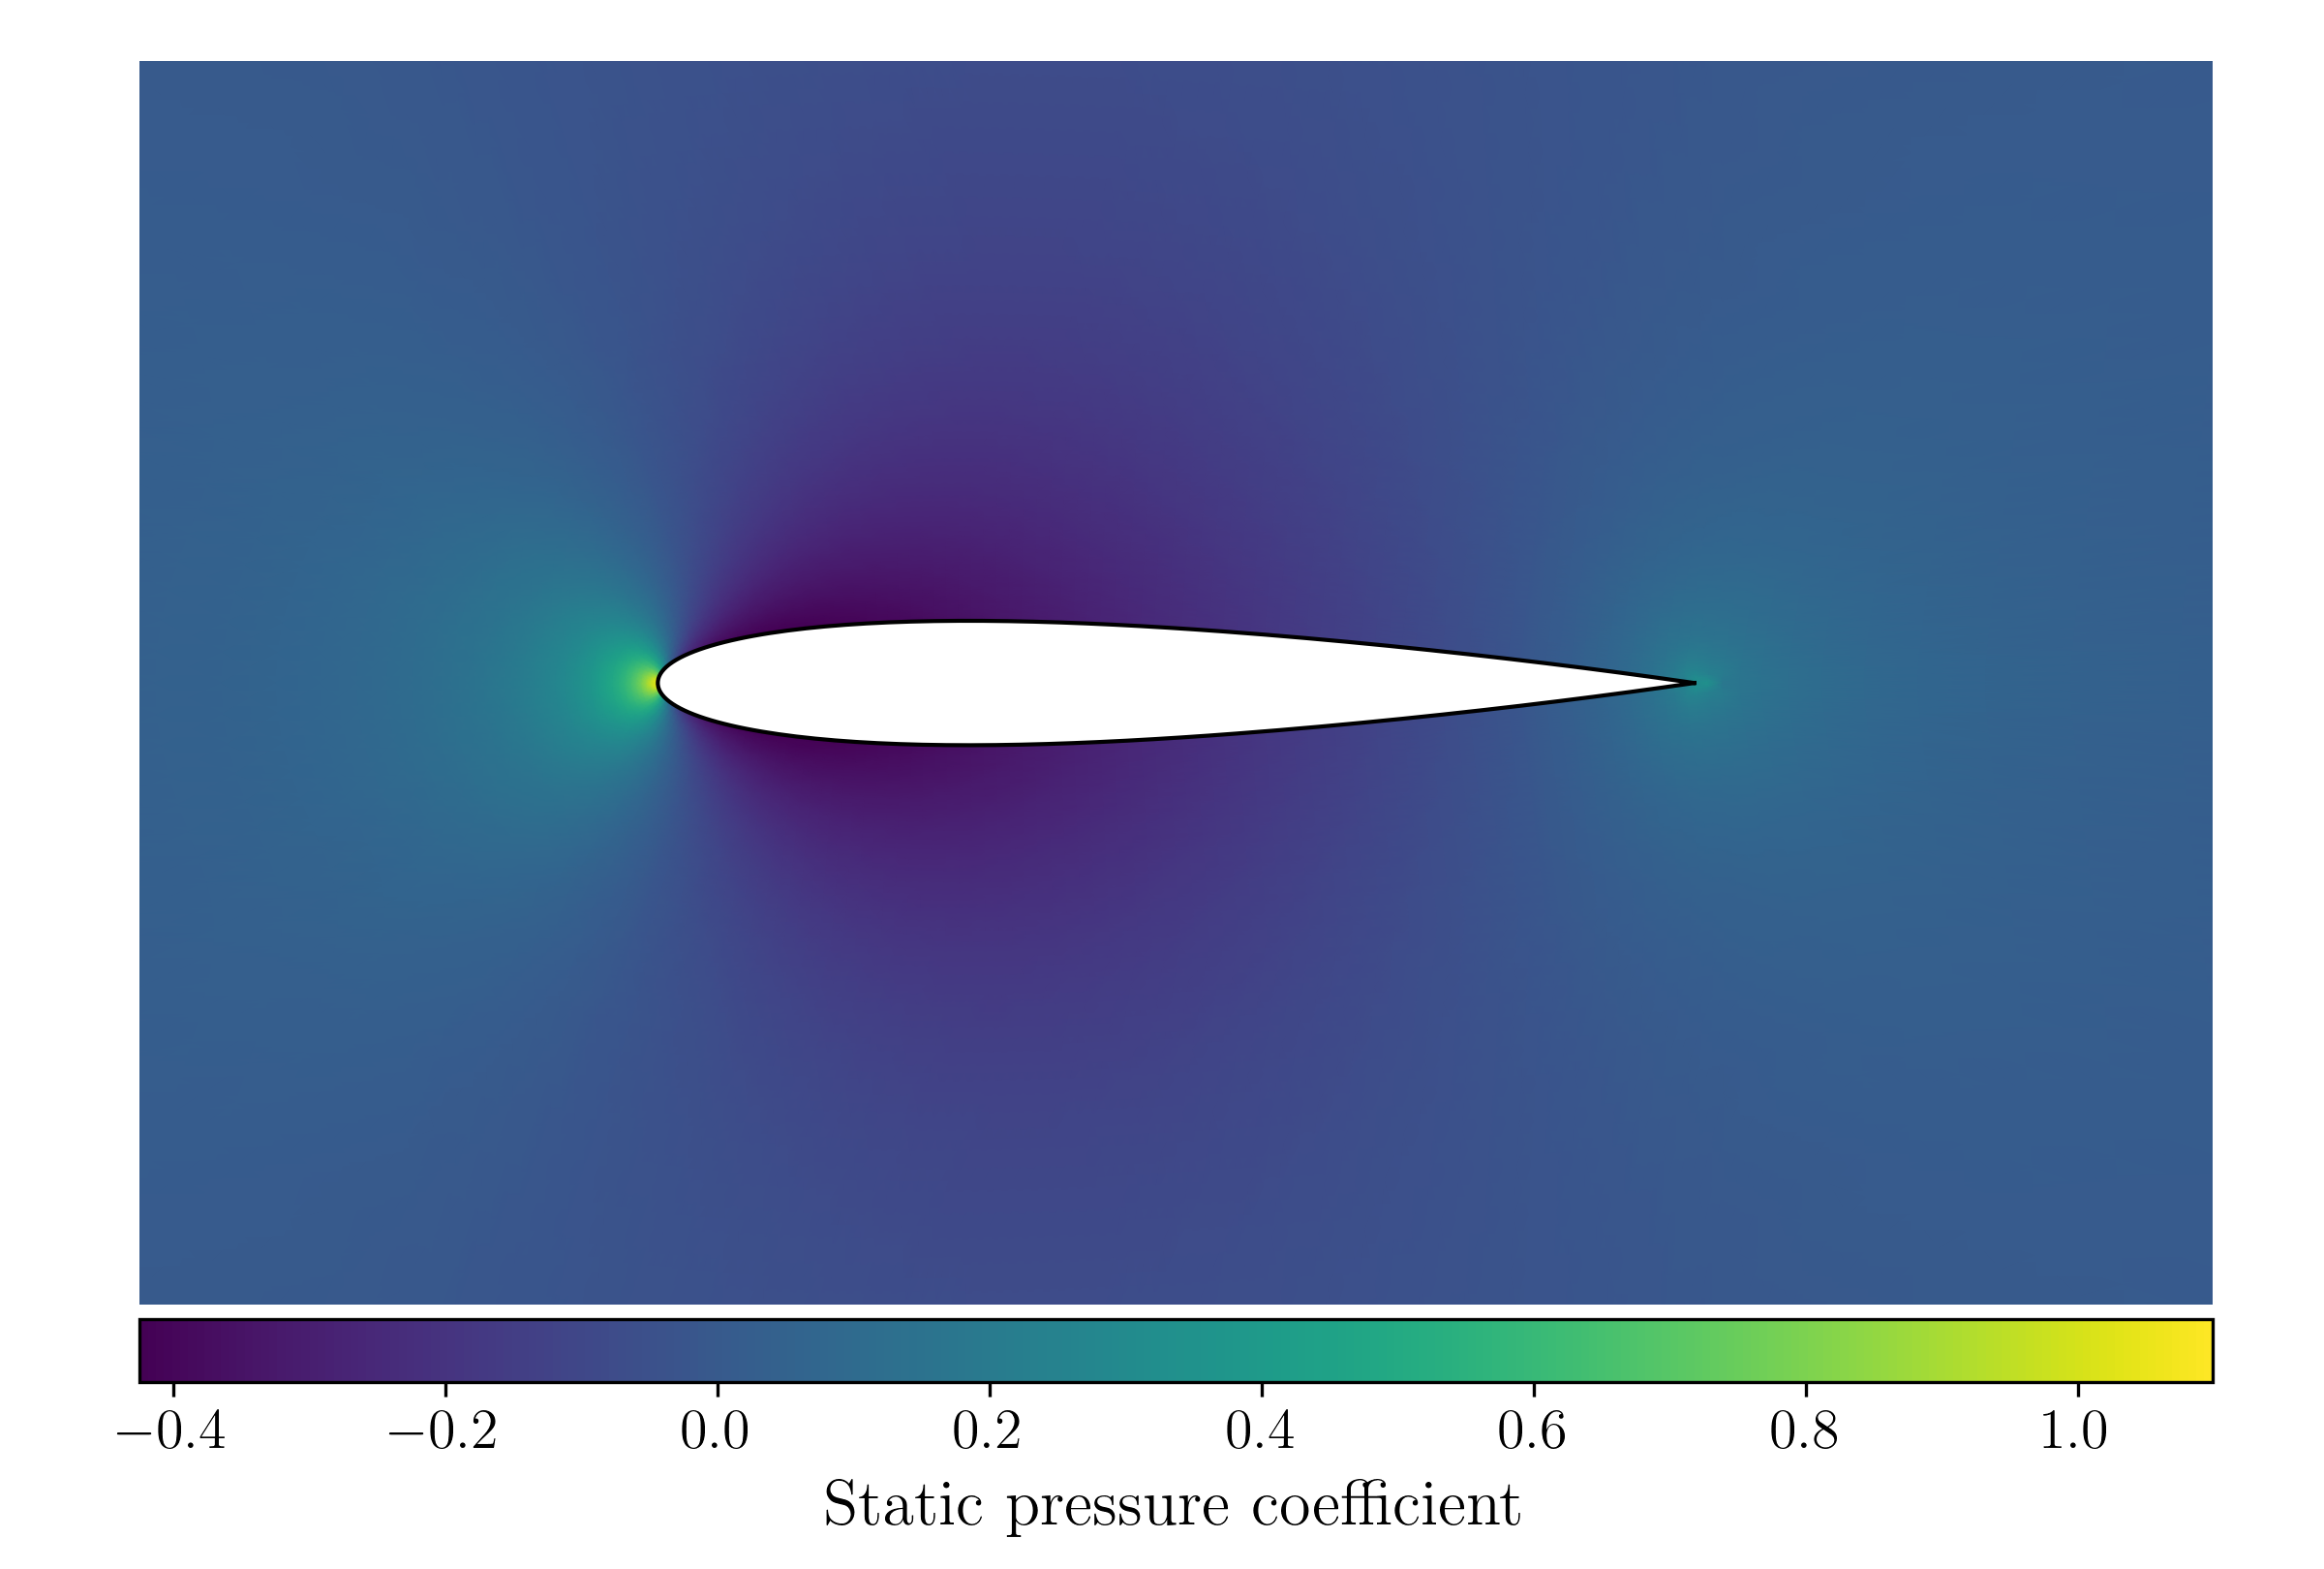
\includegraphics[width=0.99\textwidth]{figures/naca0012_cp_0.0}
        \caption{}
        \label{fig:naca0012_cp}
    \end{subfigure}
    \begin{subfigure}{0.49\textwidth}
        \centering
        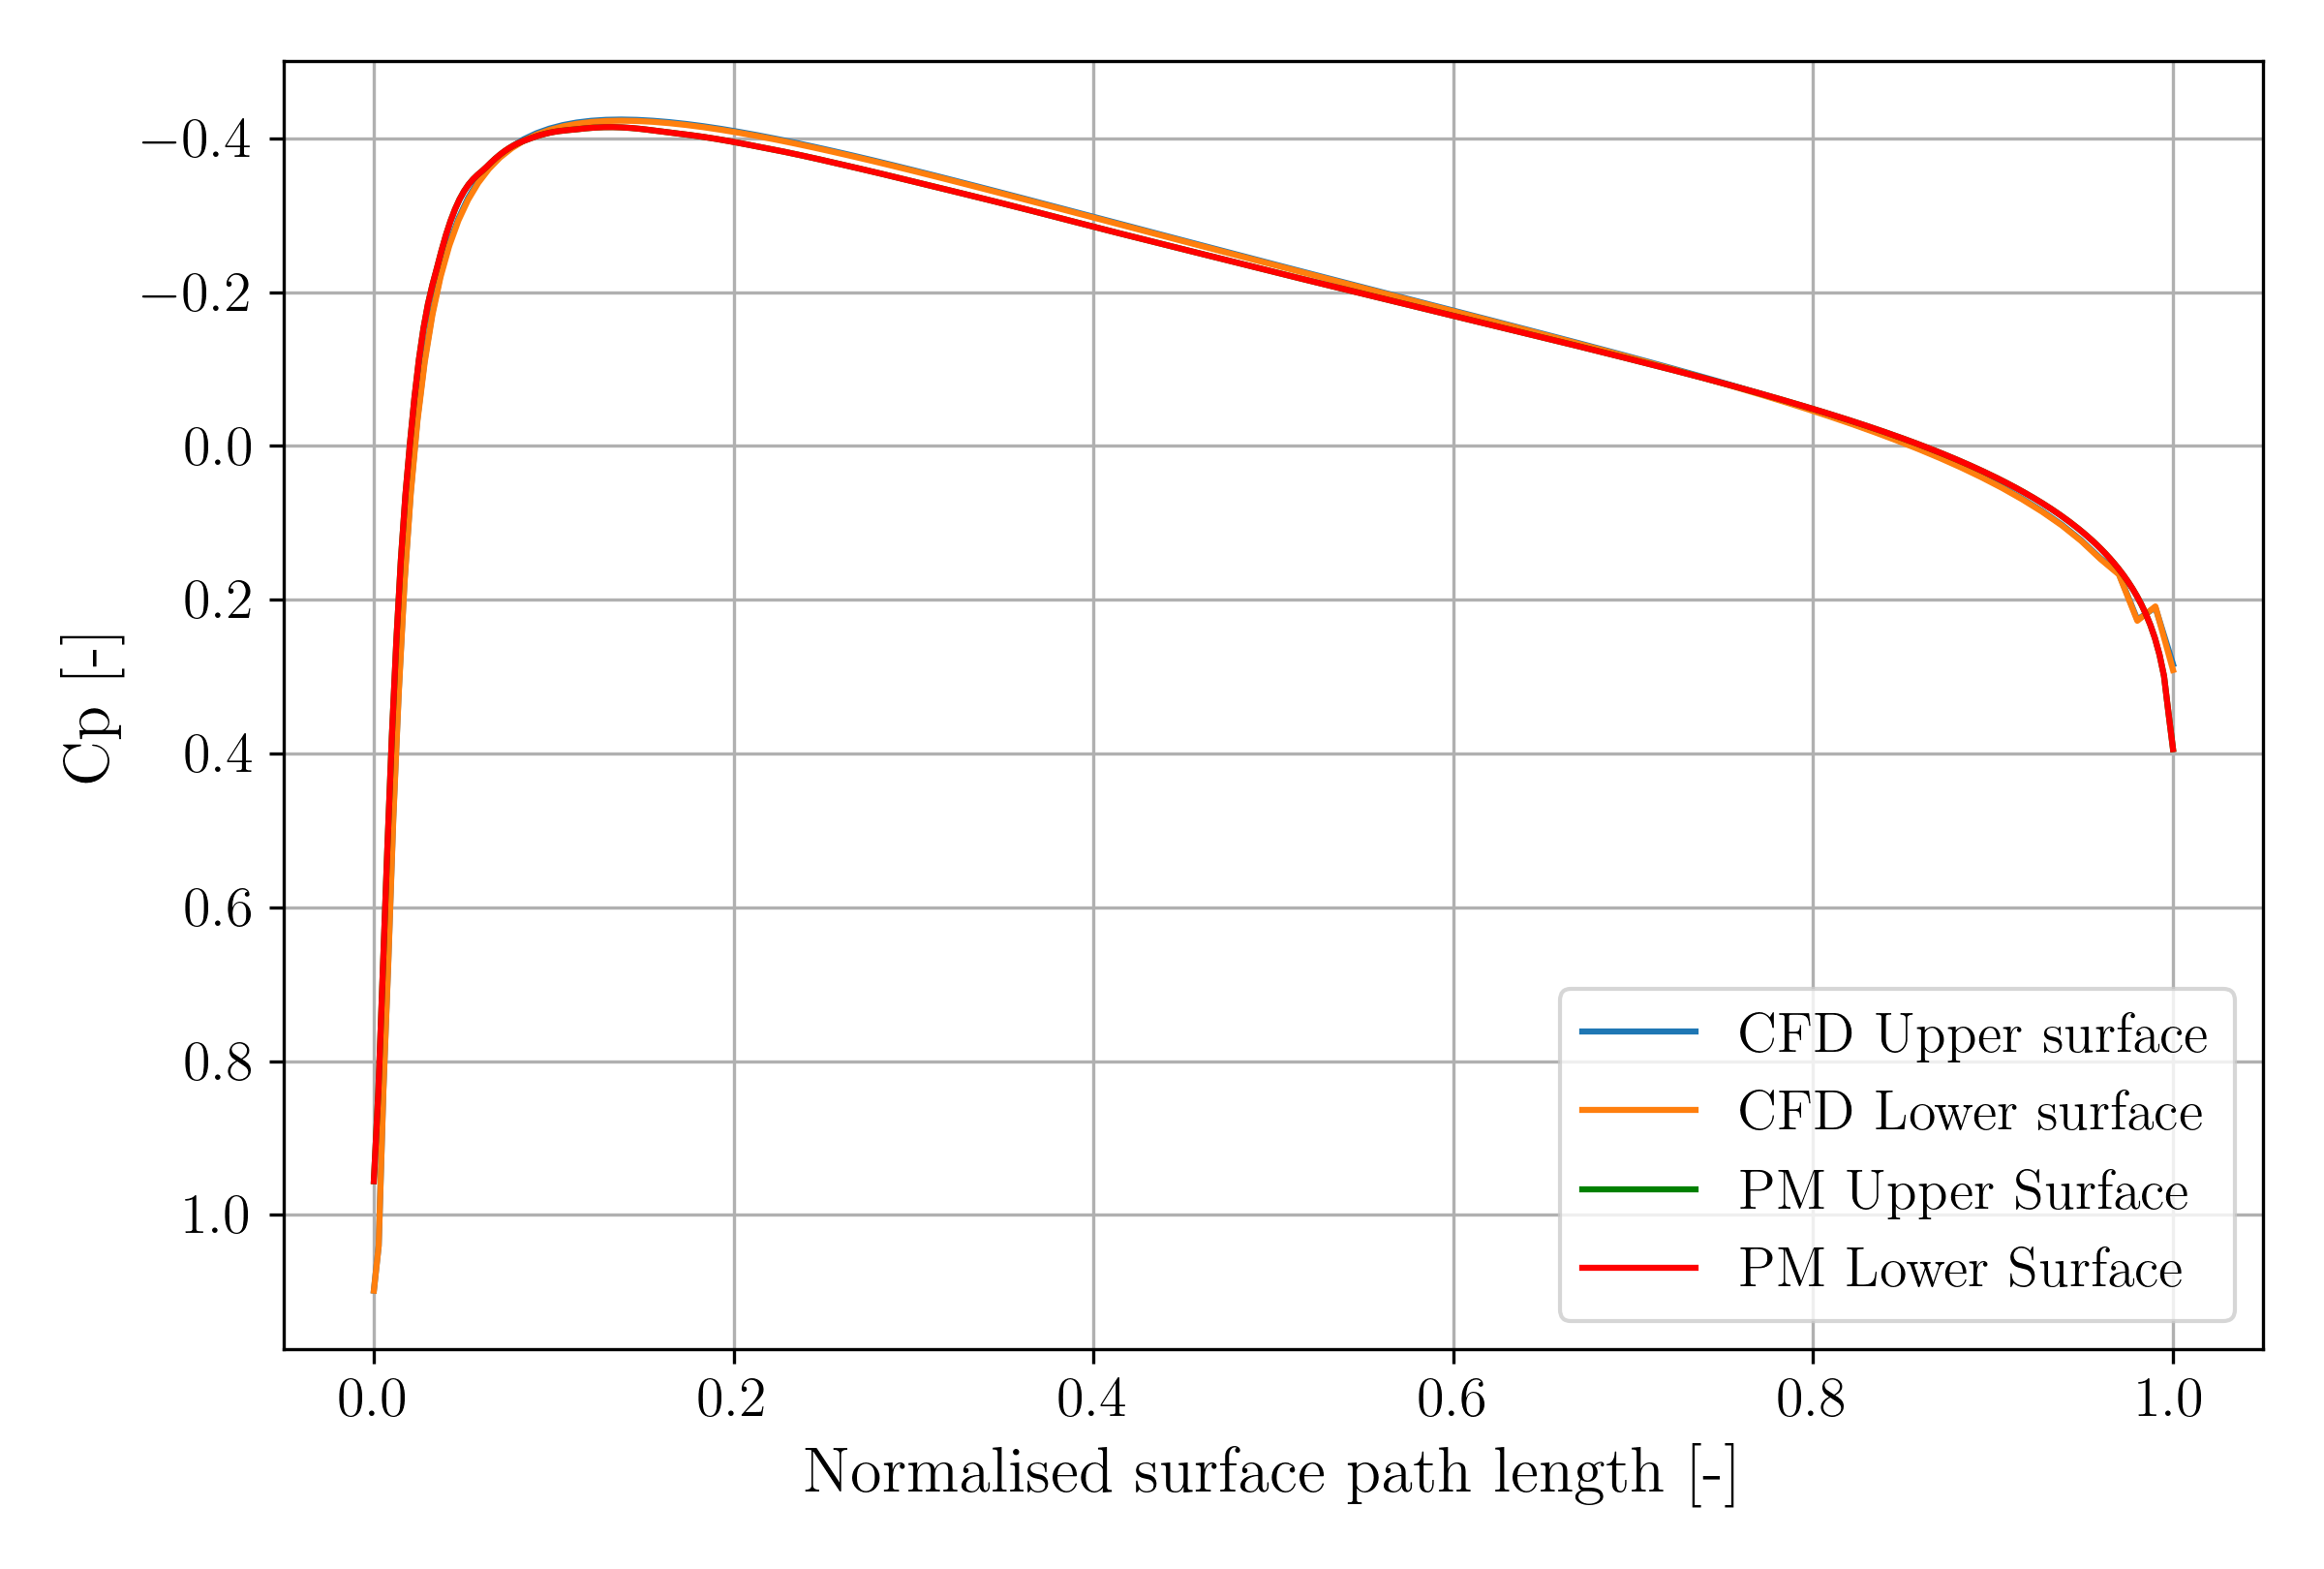
\includegraphics[width=0.99\textwidth]{figures/naca0012_surface_cp_0.0.png}
        \caption{}
        \label{fig:naca0012_surface_cp}
    \end{subfigure}
    \caption{NACA0012 test case results at $\alpha = 0^\circ$}
\end{figure}

\begin{figure}[H]
    \centering
    \begin{subfigure}{0.49\textwidth}
        \centering
        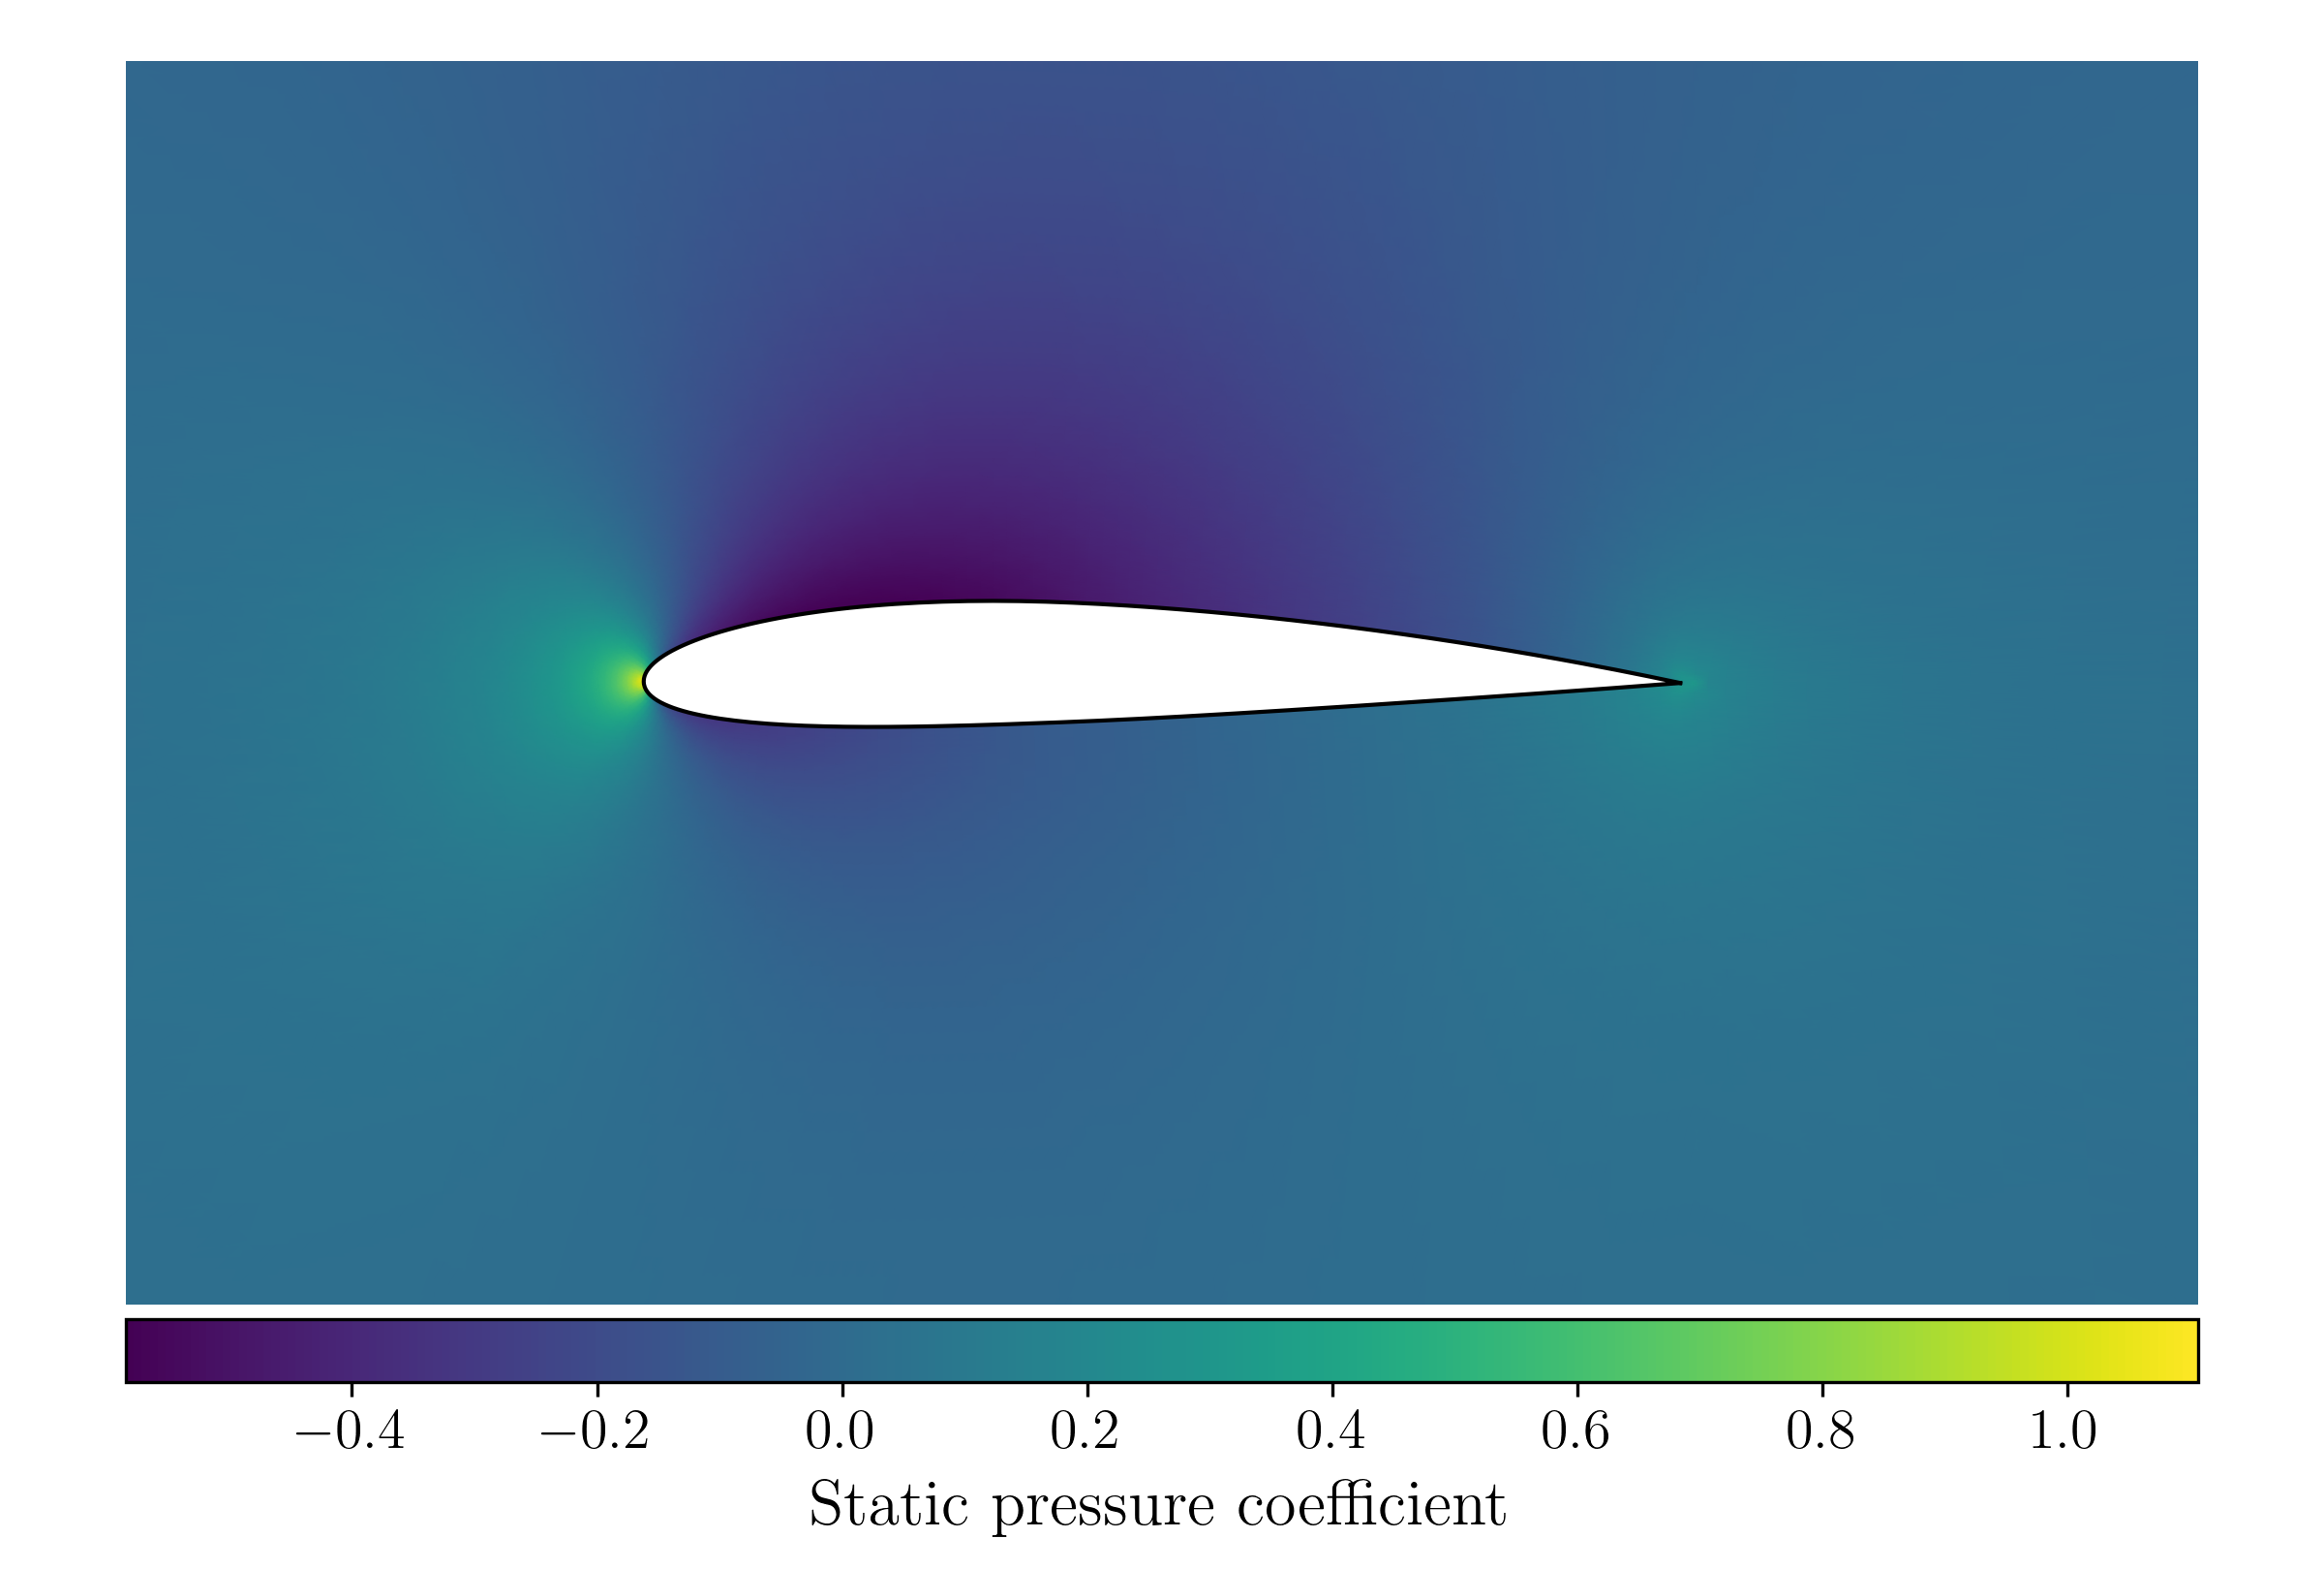
\includegraphics[width=0.99\textwidth]{figures/naca2412_cp_0.0.png}
        \caption{}
        \label{fig:naca2412_cp}
    \end{subfigure}
    \begin{subfigure}{0.49\textwidth}
        \centering
        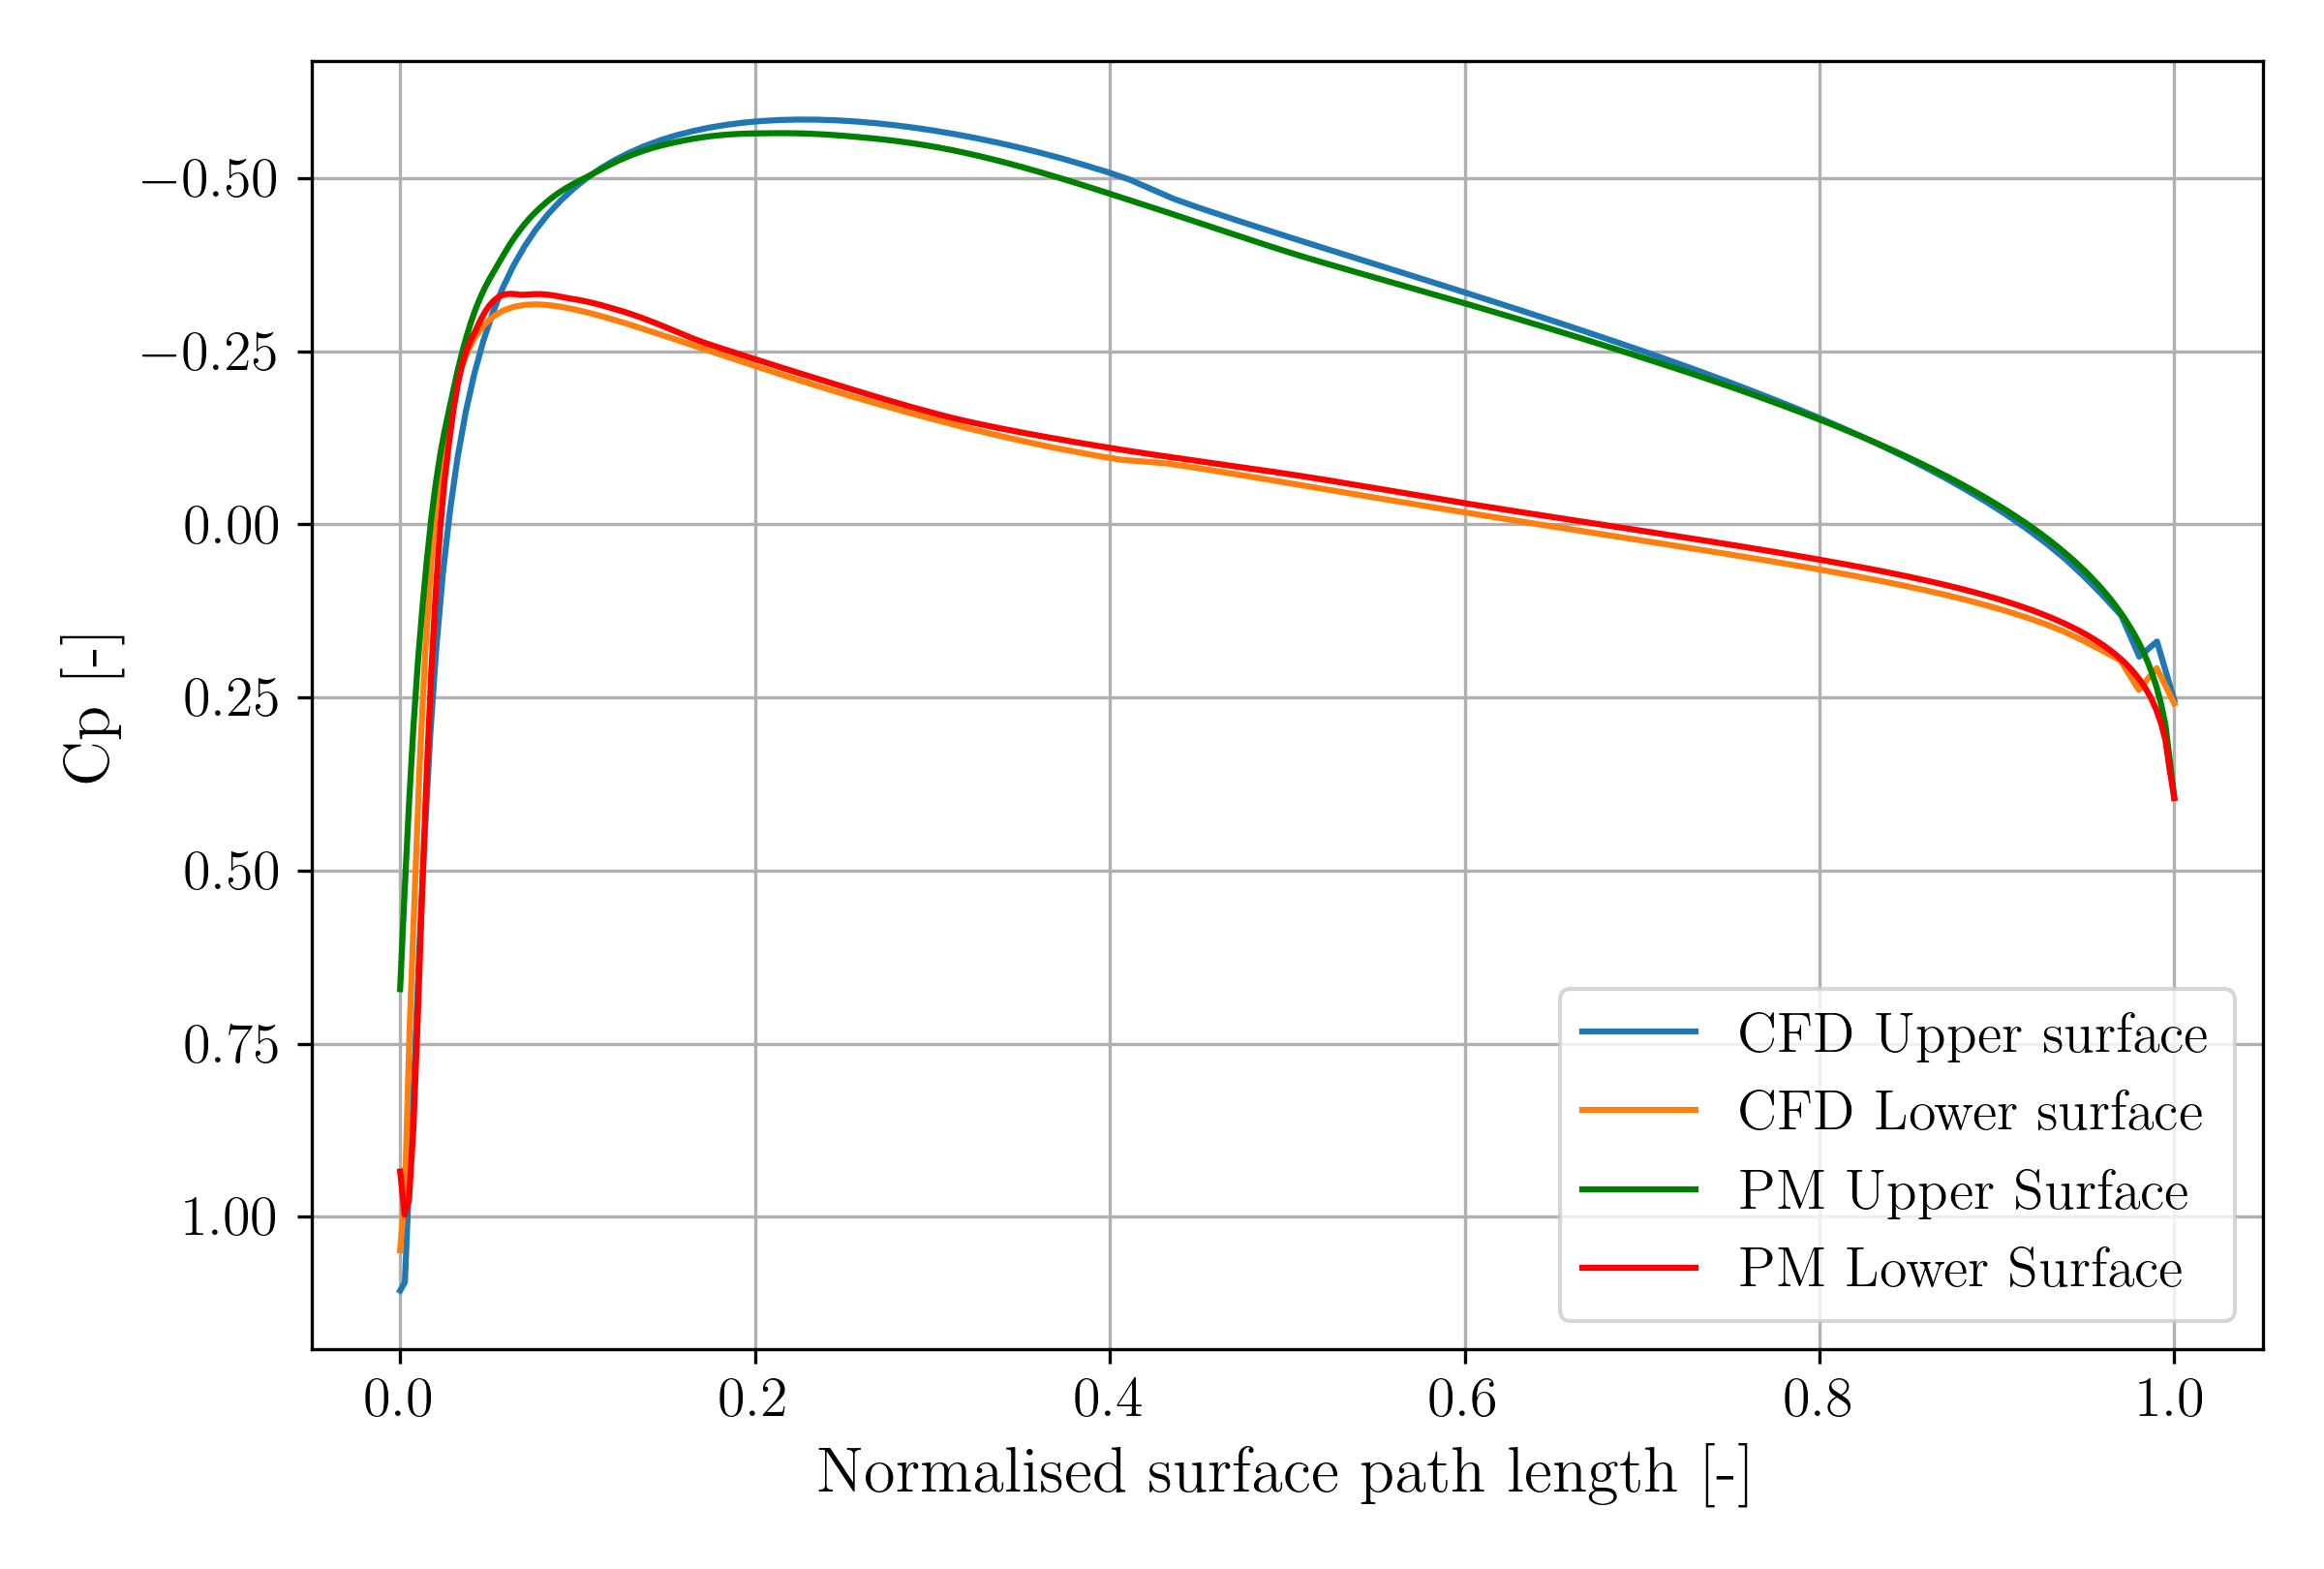
\includegraphics[width=0.99\textwidth]{figures/naca2412_surface_cp_0.0.png}
        \caption{}
        \label{fig:naca2412_surface_cp}
    \end{subfigure}
    \caption{NACA2412 test case results at $\alpha = 0^\circ$}
\end{figure}

\begin{figure}[H]
    \centering
    \begin{subfigure}{0.49\textwidth}
        \centering
        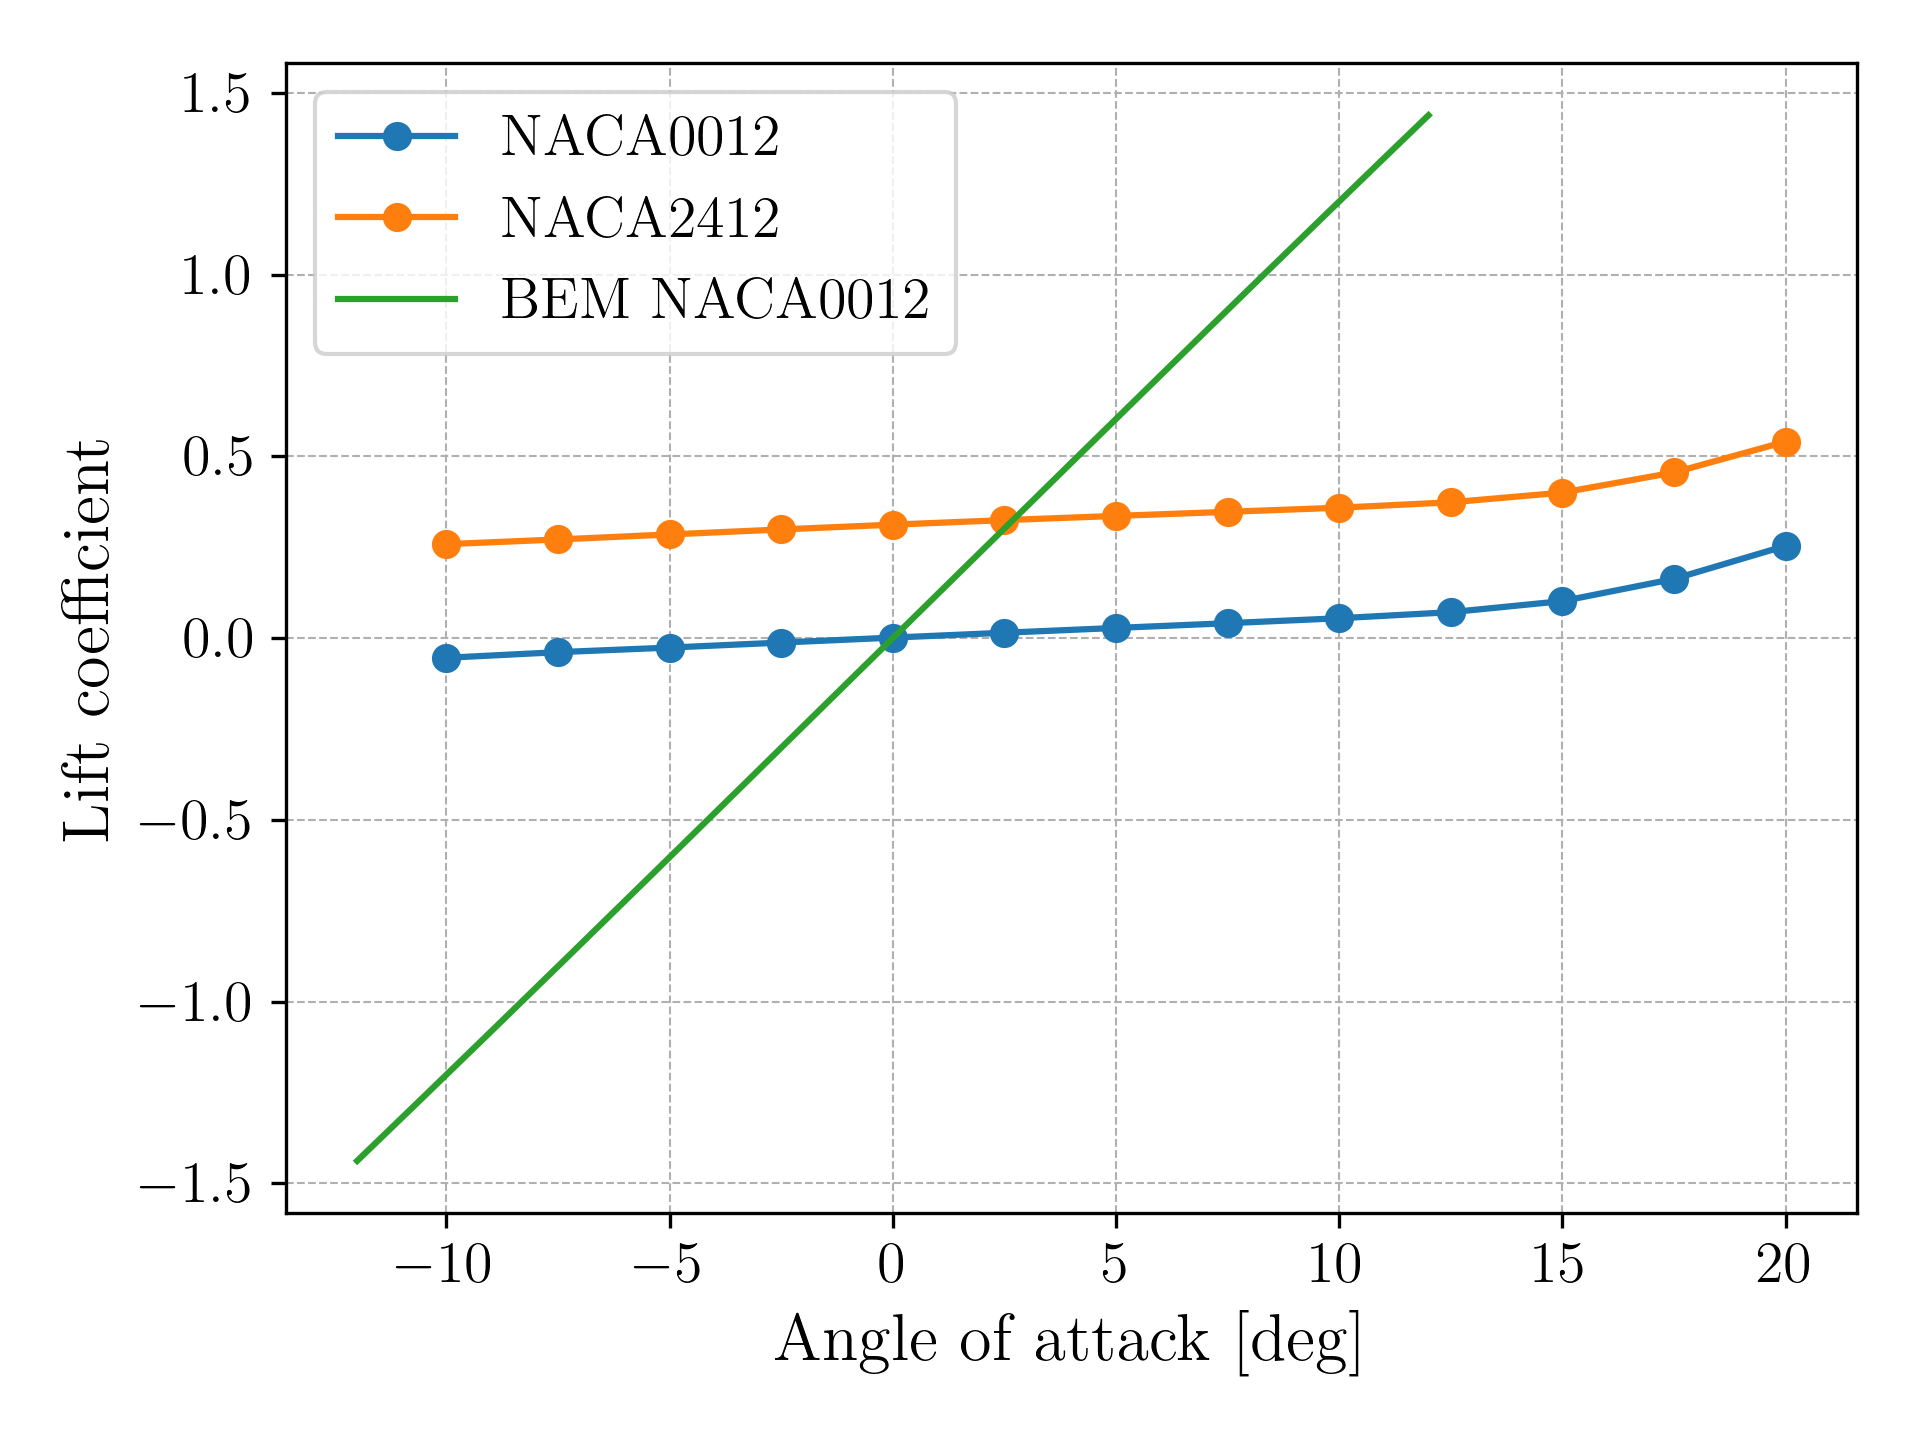
\includegraphics[width=0.99\textwidth]{figures/cl_alpha.png}
        \caption{}
        \label{fig:cl_alpha}
    \end{subfigure}
    \begin{subfigure}{0.49\textwidth}
        \centering
        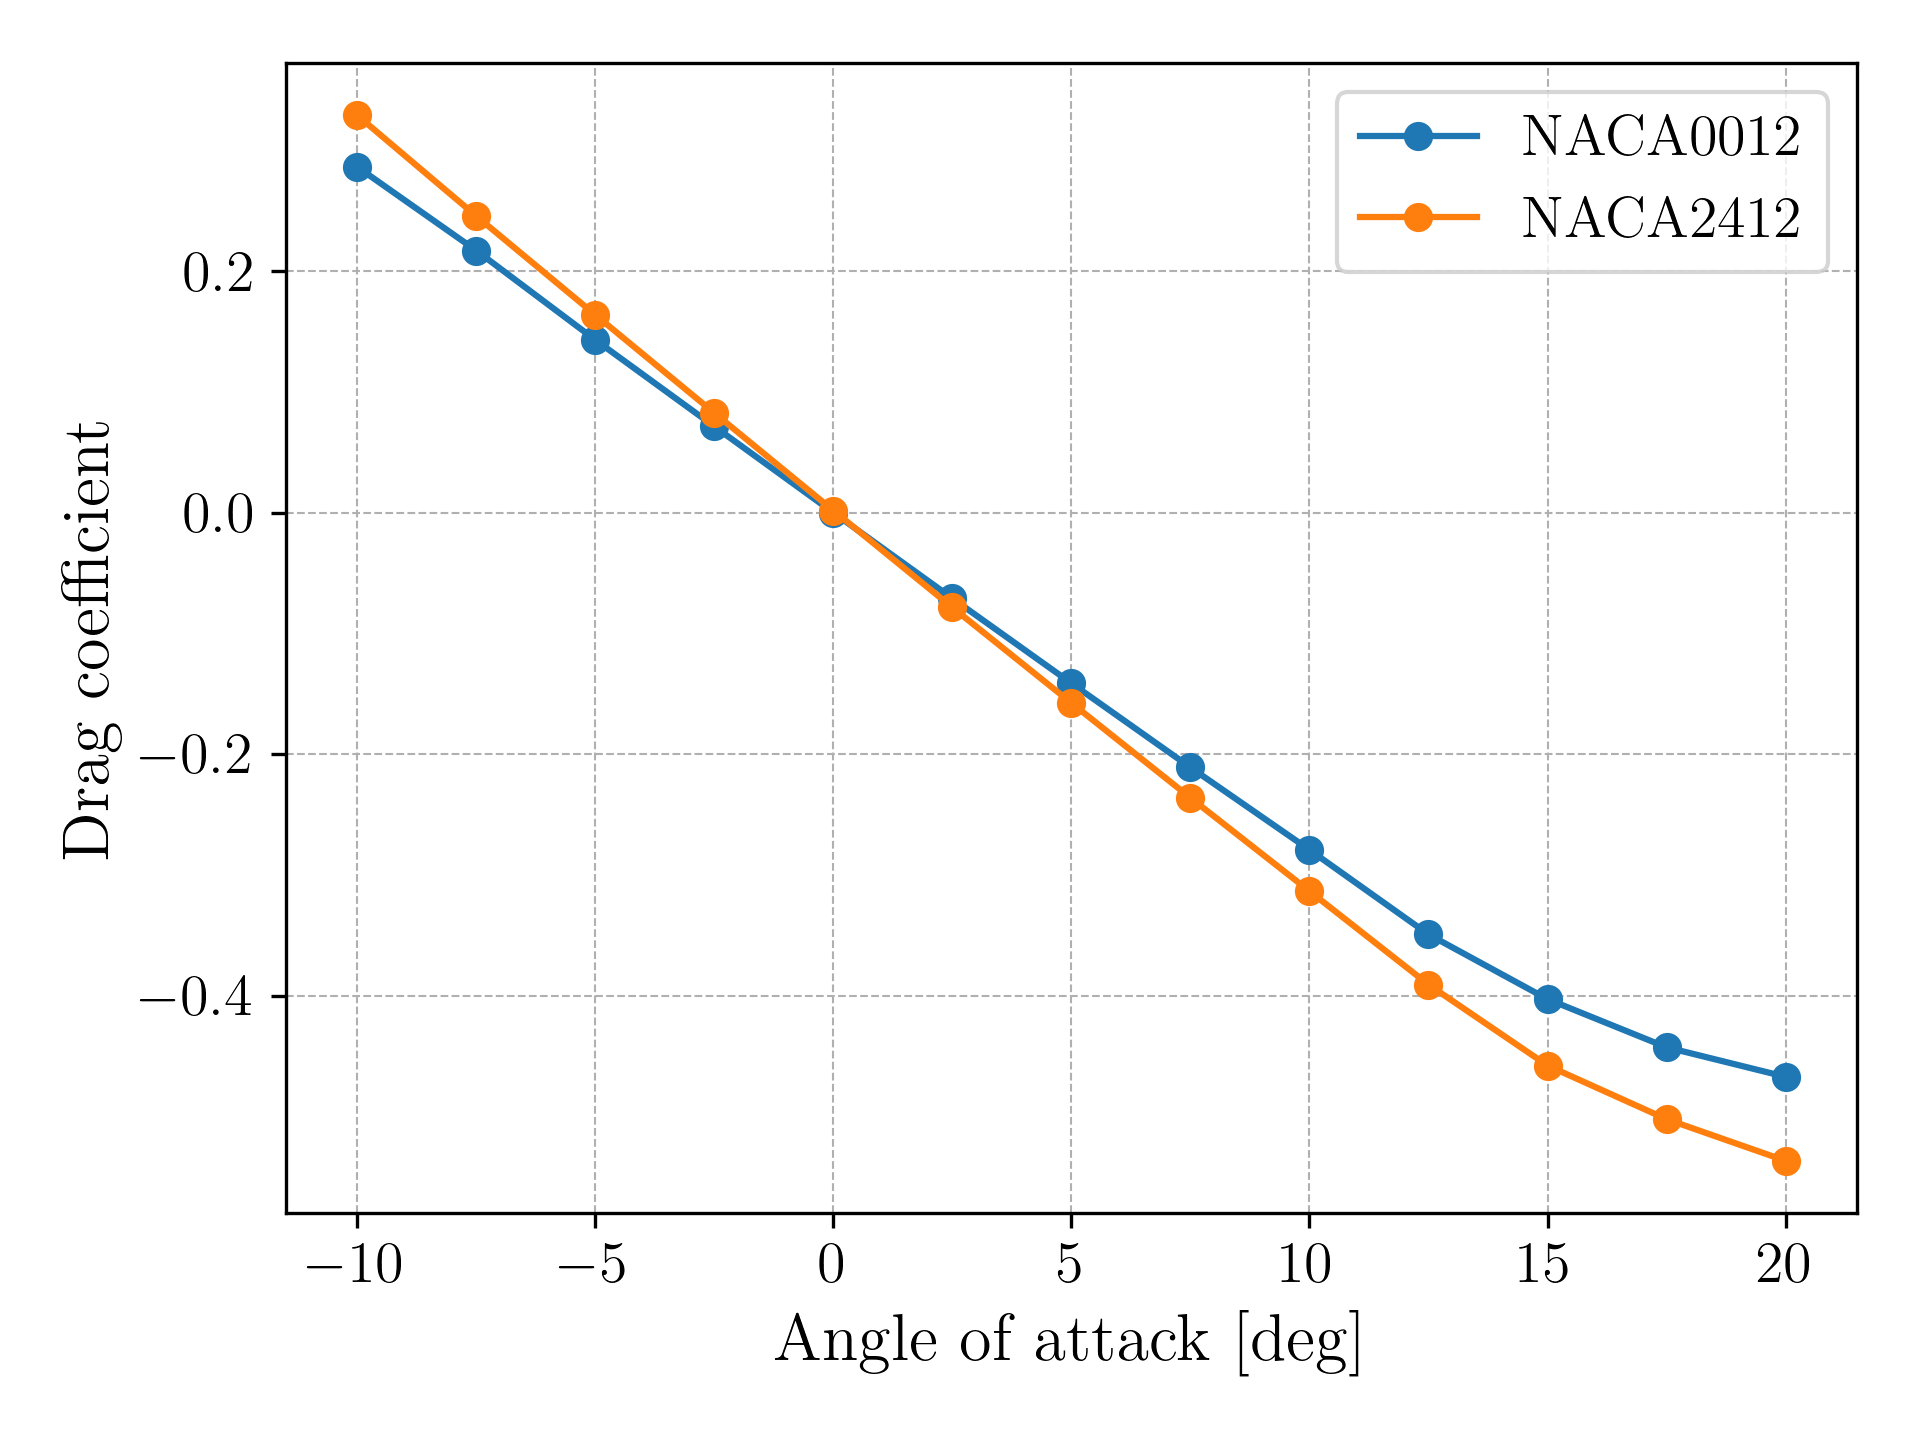
\includegraphics[width=0.99\textwidth]{figures/cd_alpha.png}
        \caption{}
        \label{fig:cd_alpha}
    \end{subfigure}
    \caption{NACA2412 test case results}
\end{figure}

\begin{figure}[H]
    \centering
    \begin{subfigure}{0.49\textwidth}
        \centering
        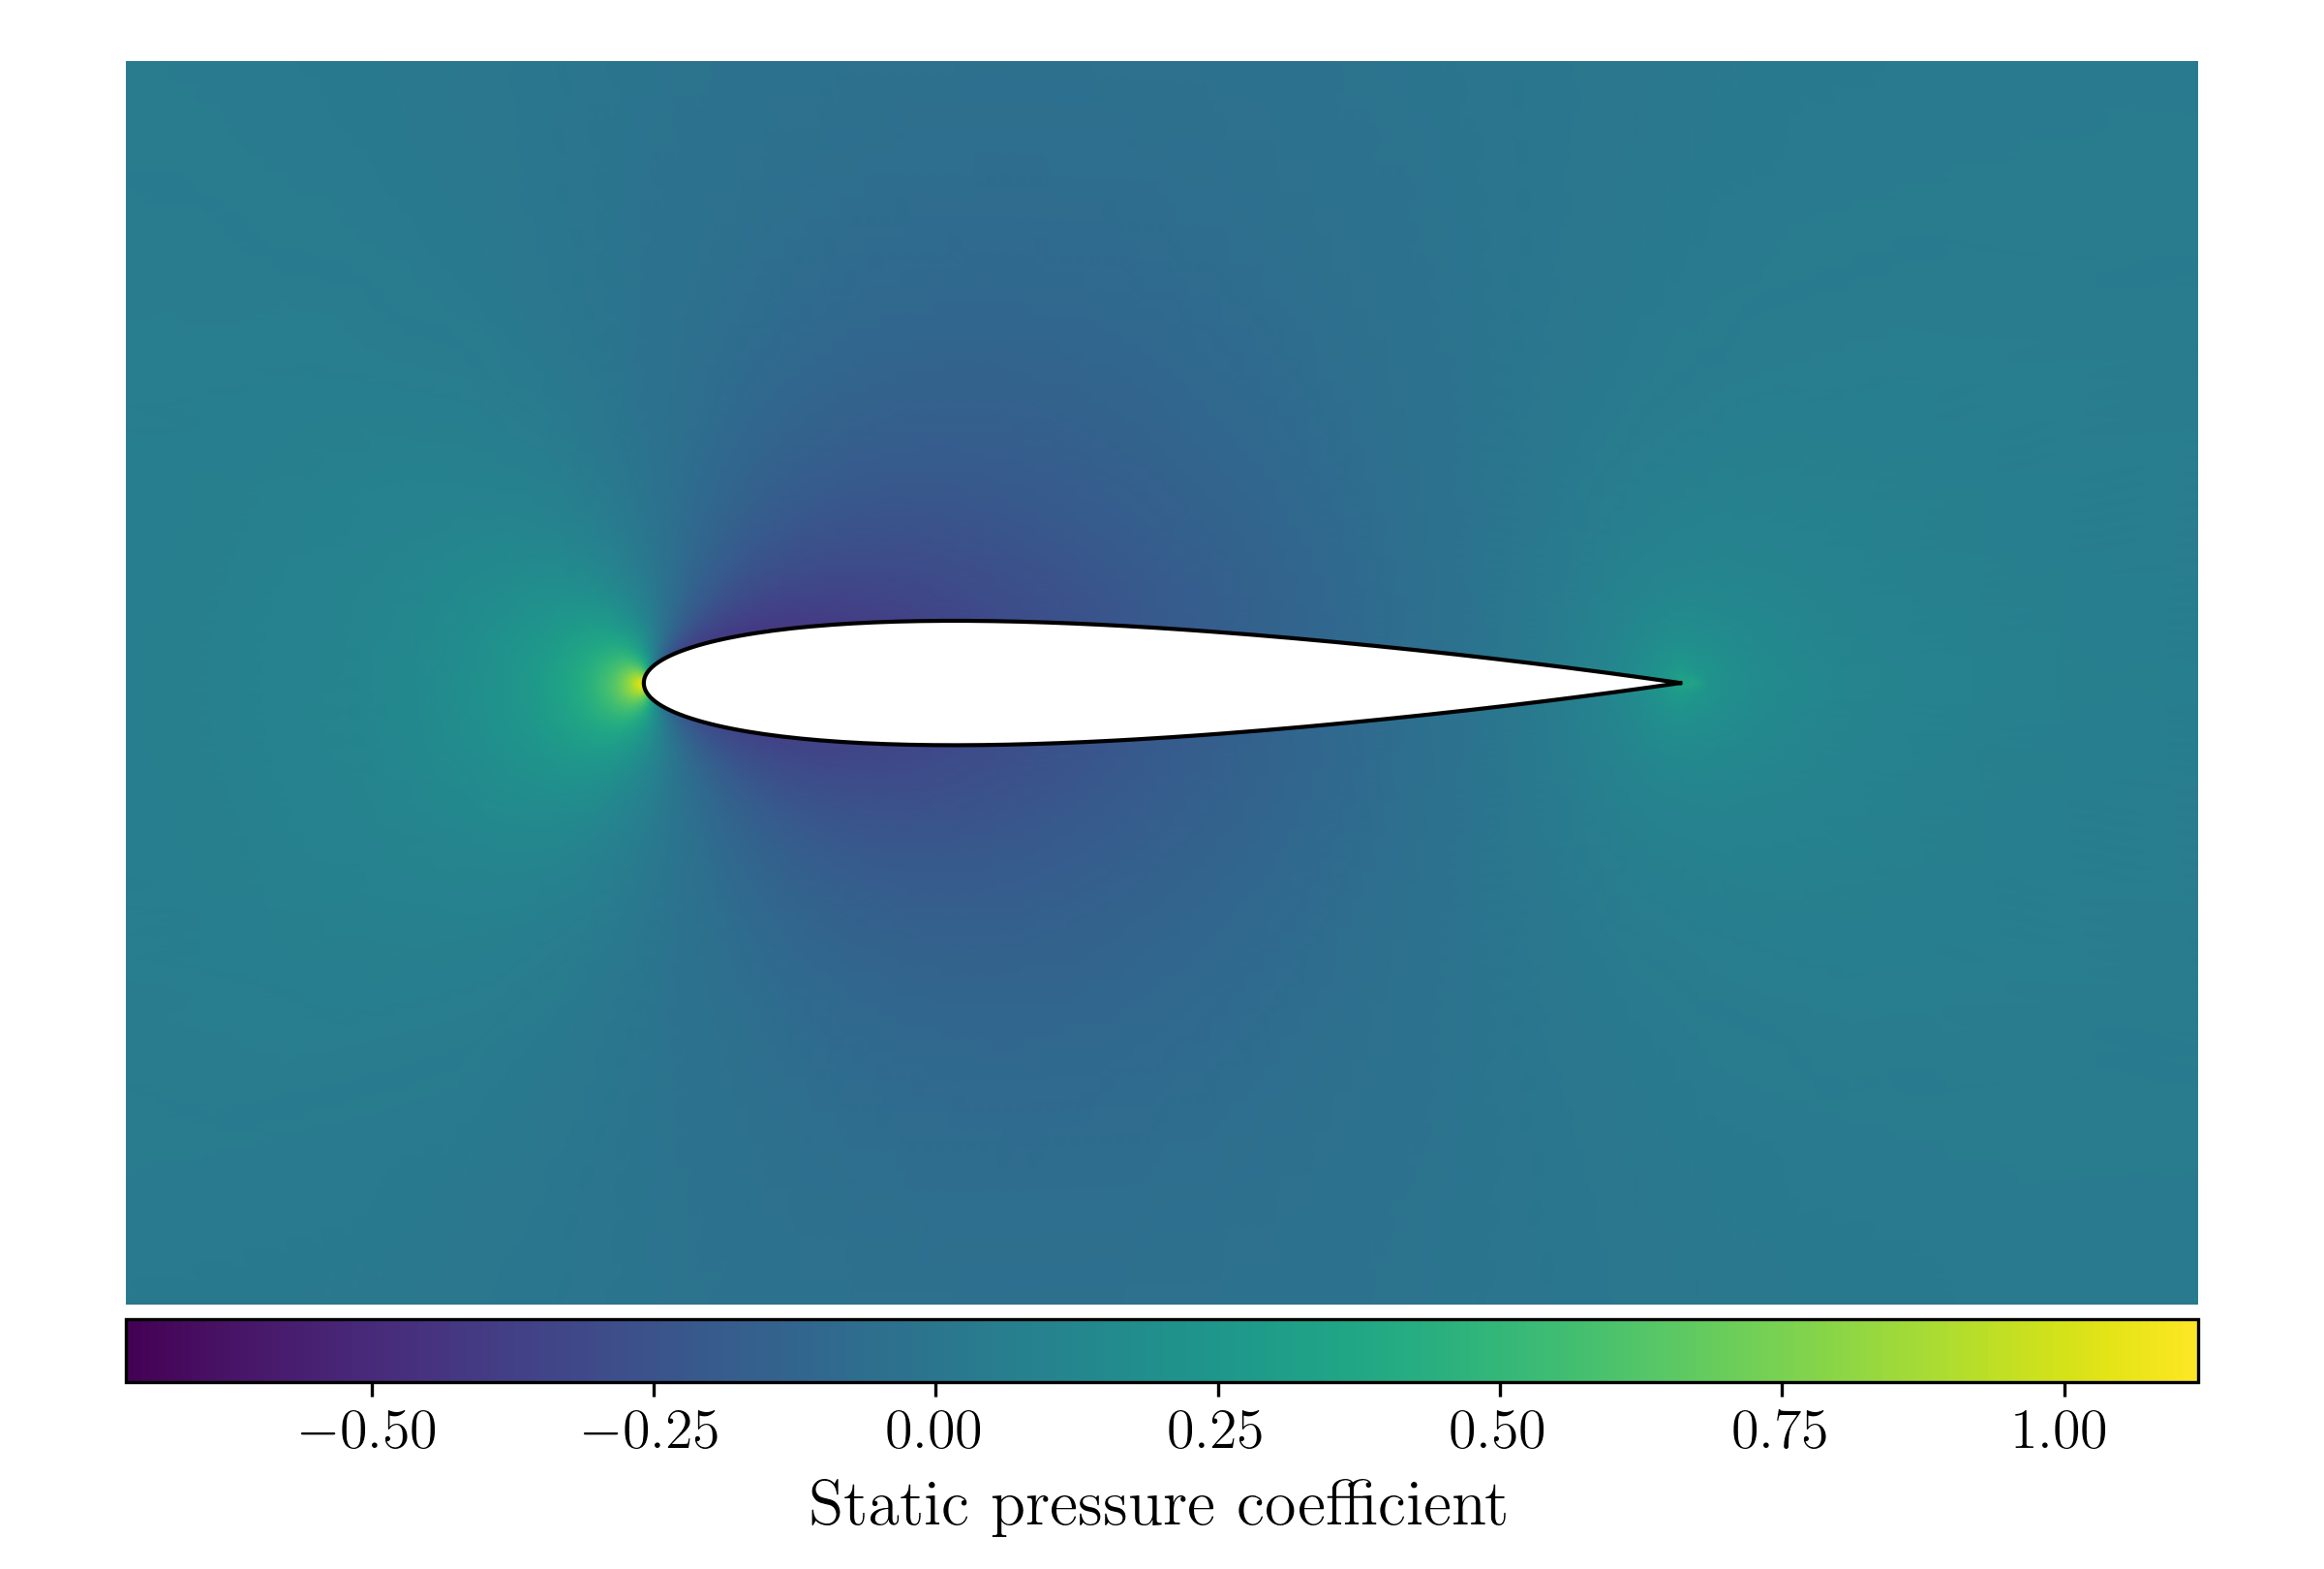
\includegraphics[width=0.99\textwidth]{figures/naca0012_cp_5.0.png}
        \caption{}
        \label{fig:naca0012_cp5}
    \end{subfigure}
    \begin{subfigure}{0.49\textwidth}
        \centering
        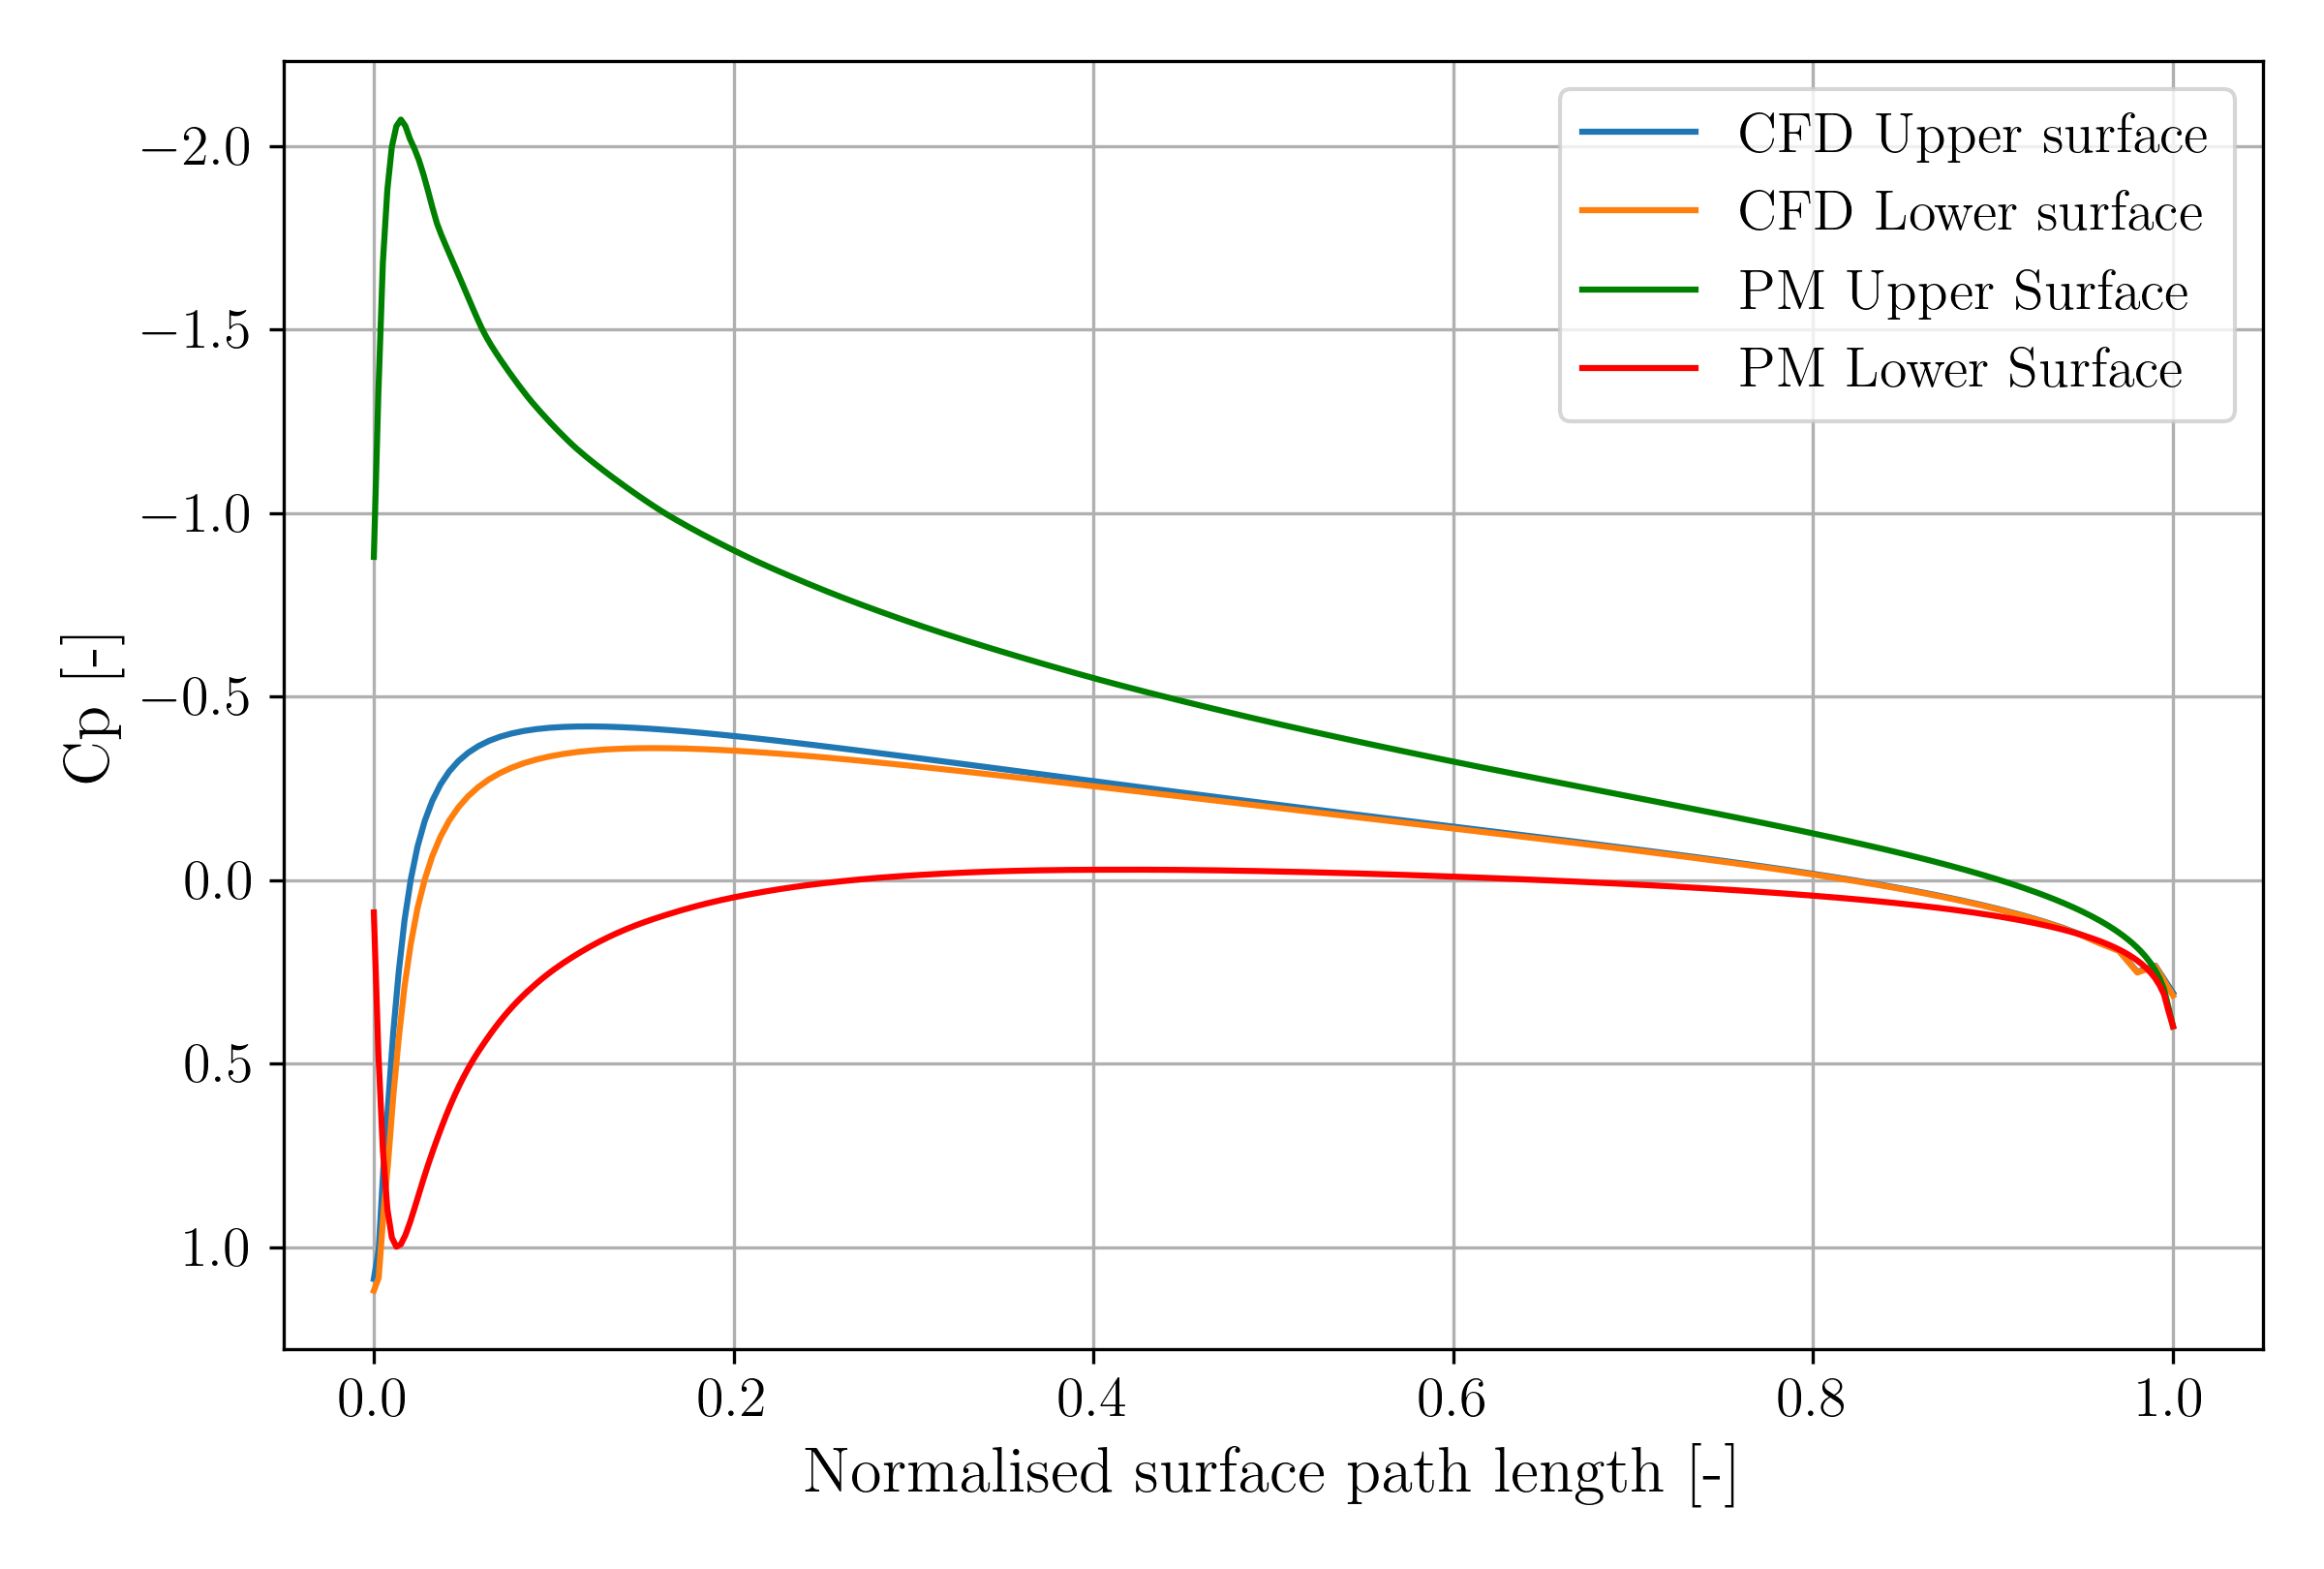
\includegraphics[width=0.99\textwidth]{figures/naca0012_surface_cp_5.0.png}
        \caption{}
        \label{fig:naca0012_surface_cp5}
    \end{subfigure}
    \caption{NACA0012 test case results at $\alpha = 5^\circ$}
\end{figure}

\begin{figure}[H]
    \centering
    \begin{subfigure}{0.49\textwidth}
        \centering
        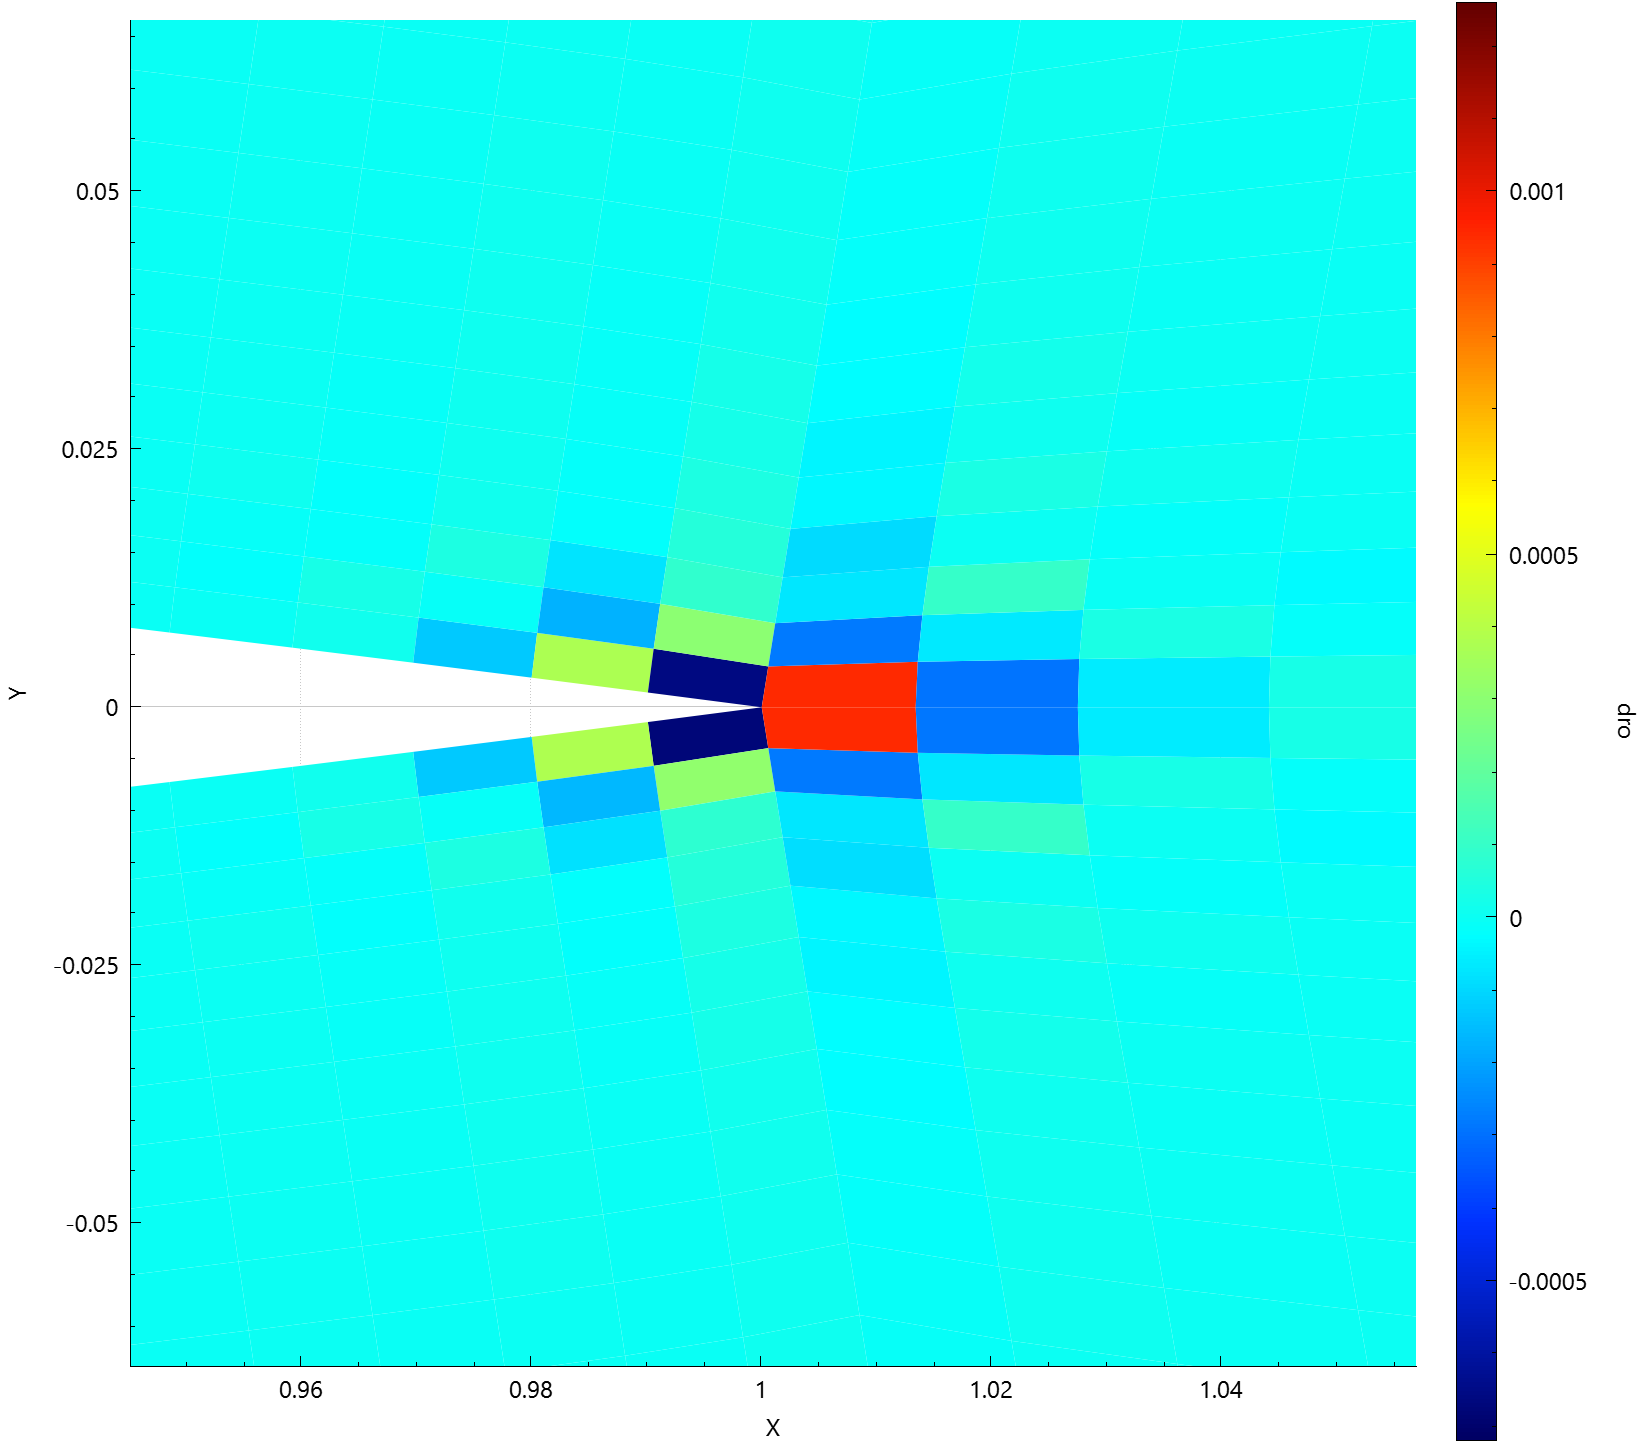
\includegraphics[width=0.8\textwidth]{figures/kutta.png}
        \caption{Trailing edge residual map}
        \label{fig:kutta}
    \end{subfigure}
    \begin{subfigure}{0.49\textwidth}
        \centering
        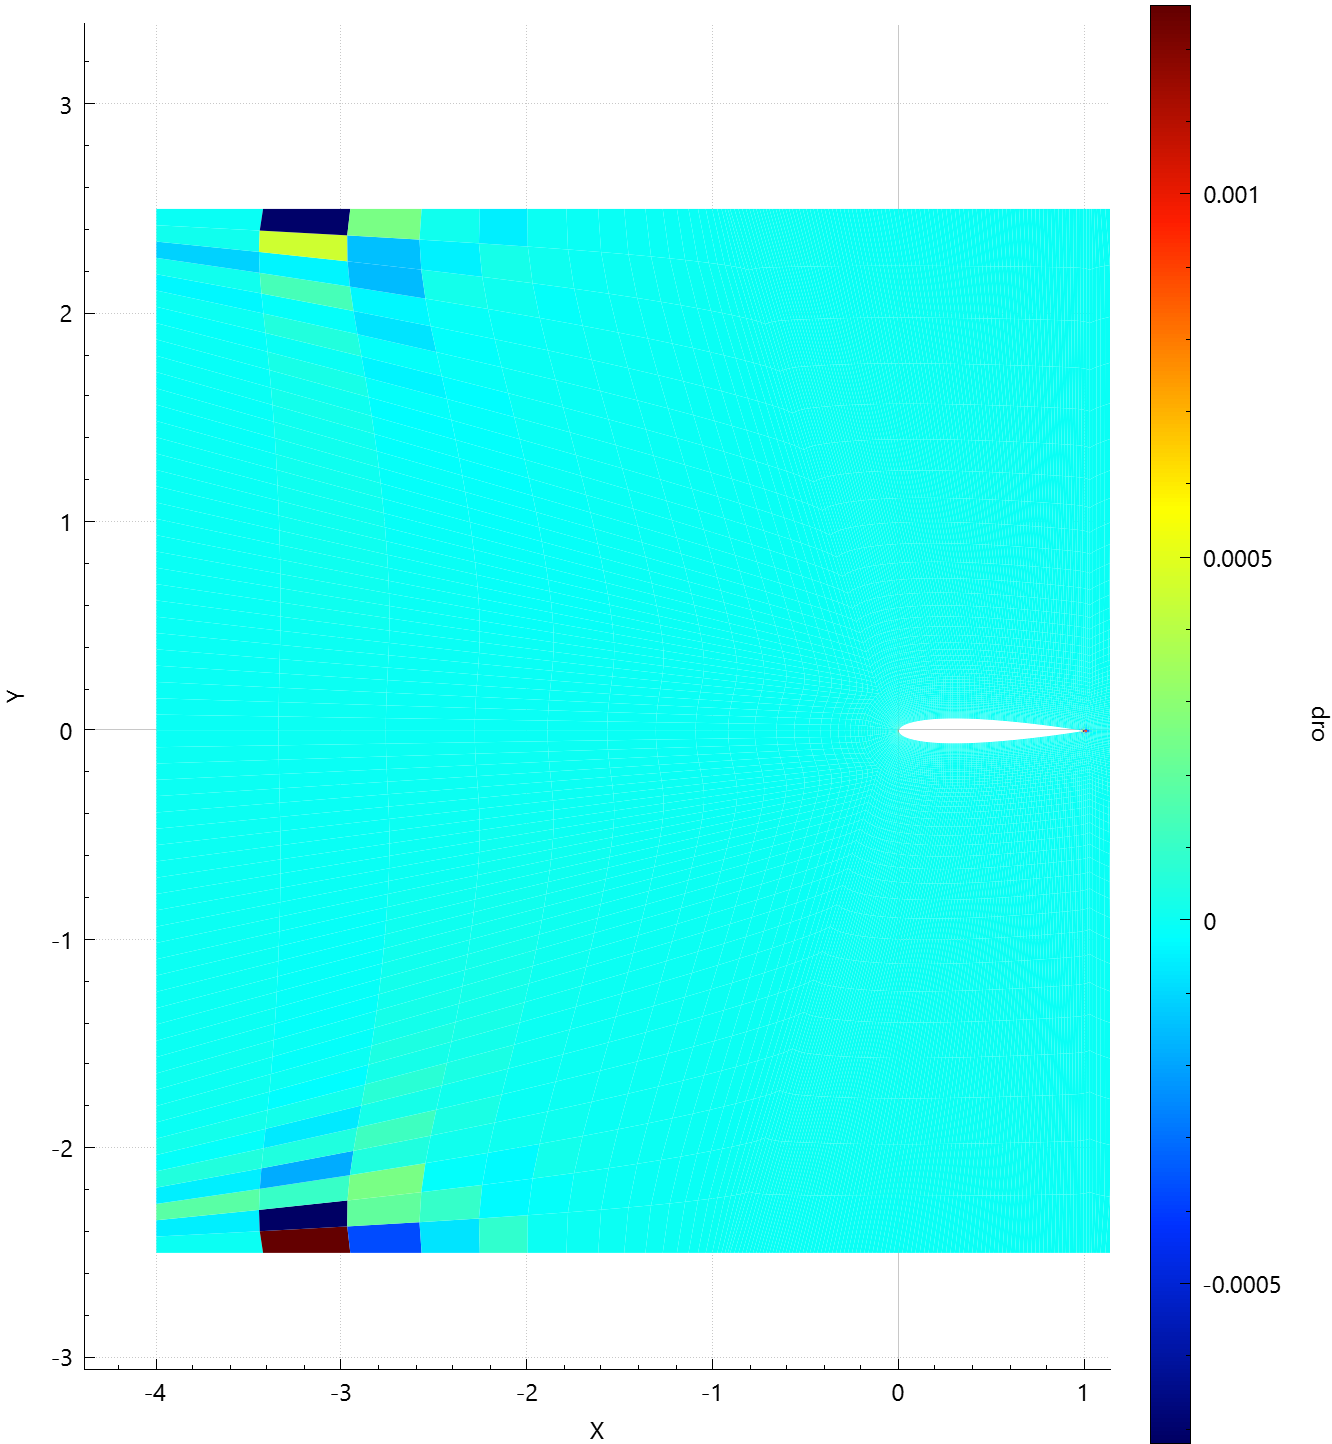
\includegraphics[width=0.7\textwidth]{figures/corner.png}
        \caption{Domain corner residual map}
        \label{fig:corners}
    \end{subfigure}
    \caption{Residual maps for NACA0012 at $\alpha = 0^\circ$}
    \label{fig:naca_residual_maps}
\end{figure}

\subsection{Turbine}

\begin{figure}[H]
    \centering
    \begin{subfigure}{0.44\textwidth}
        \centering
        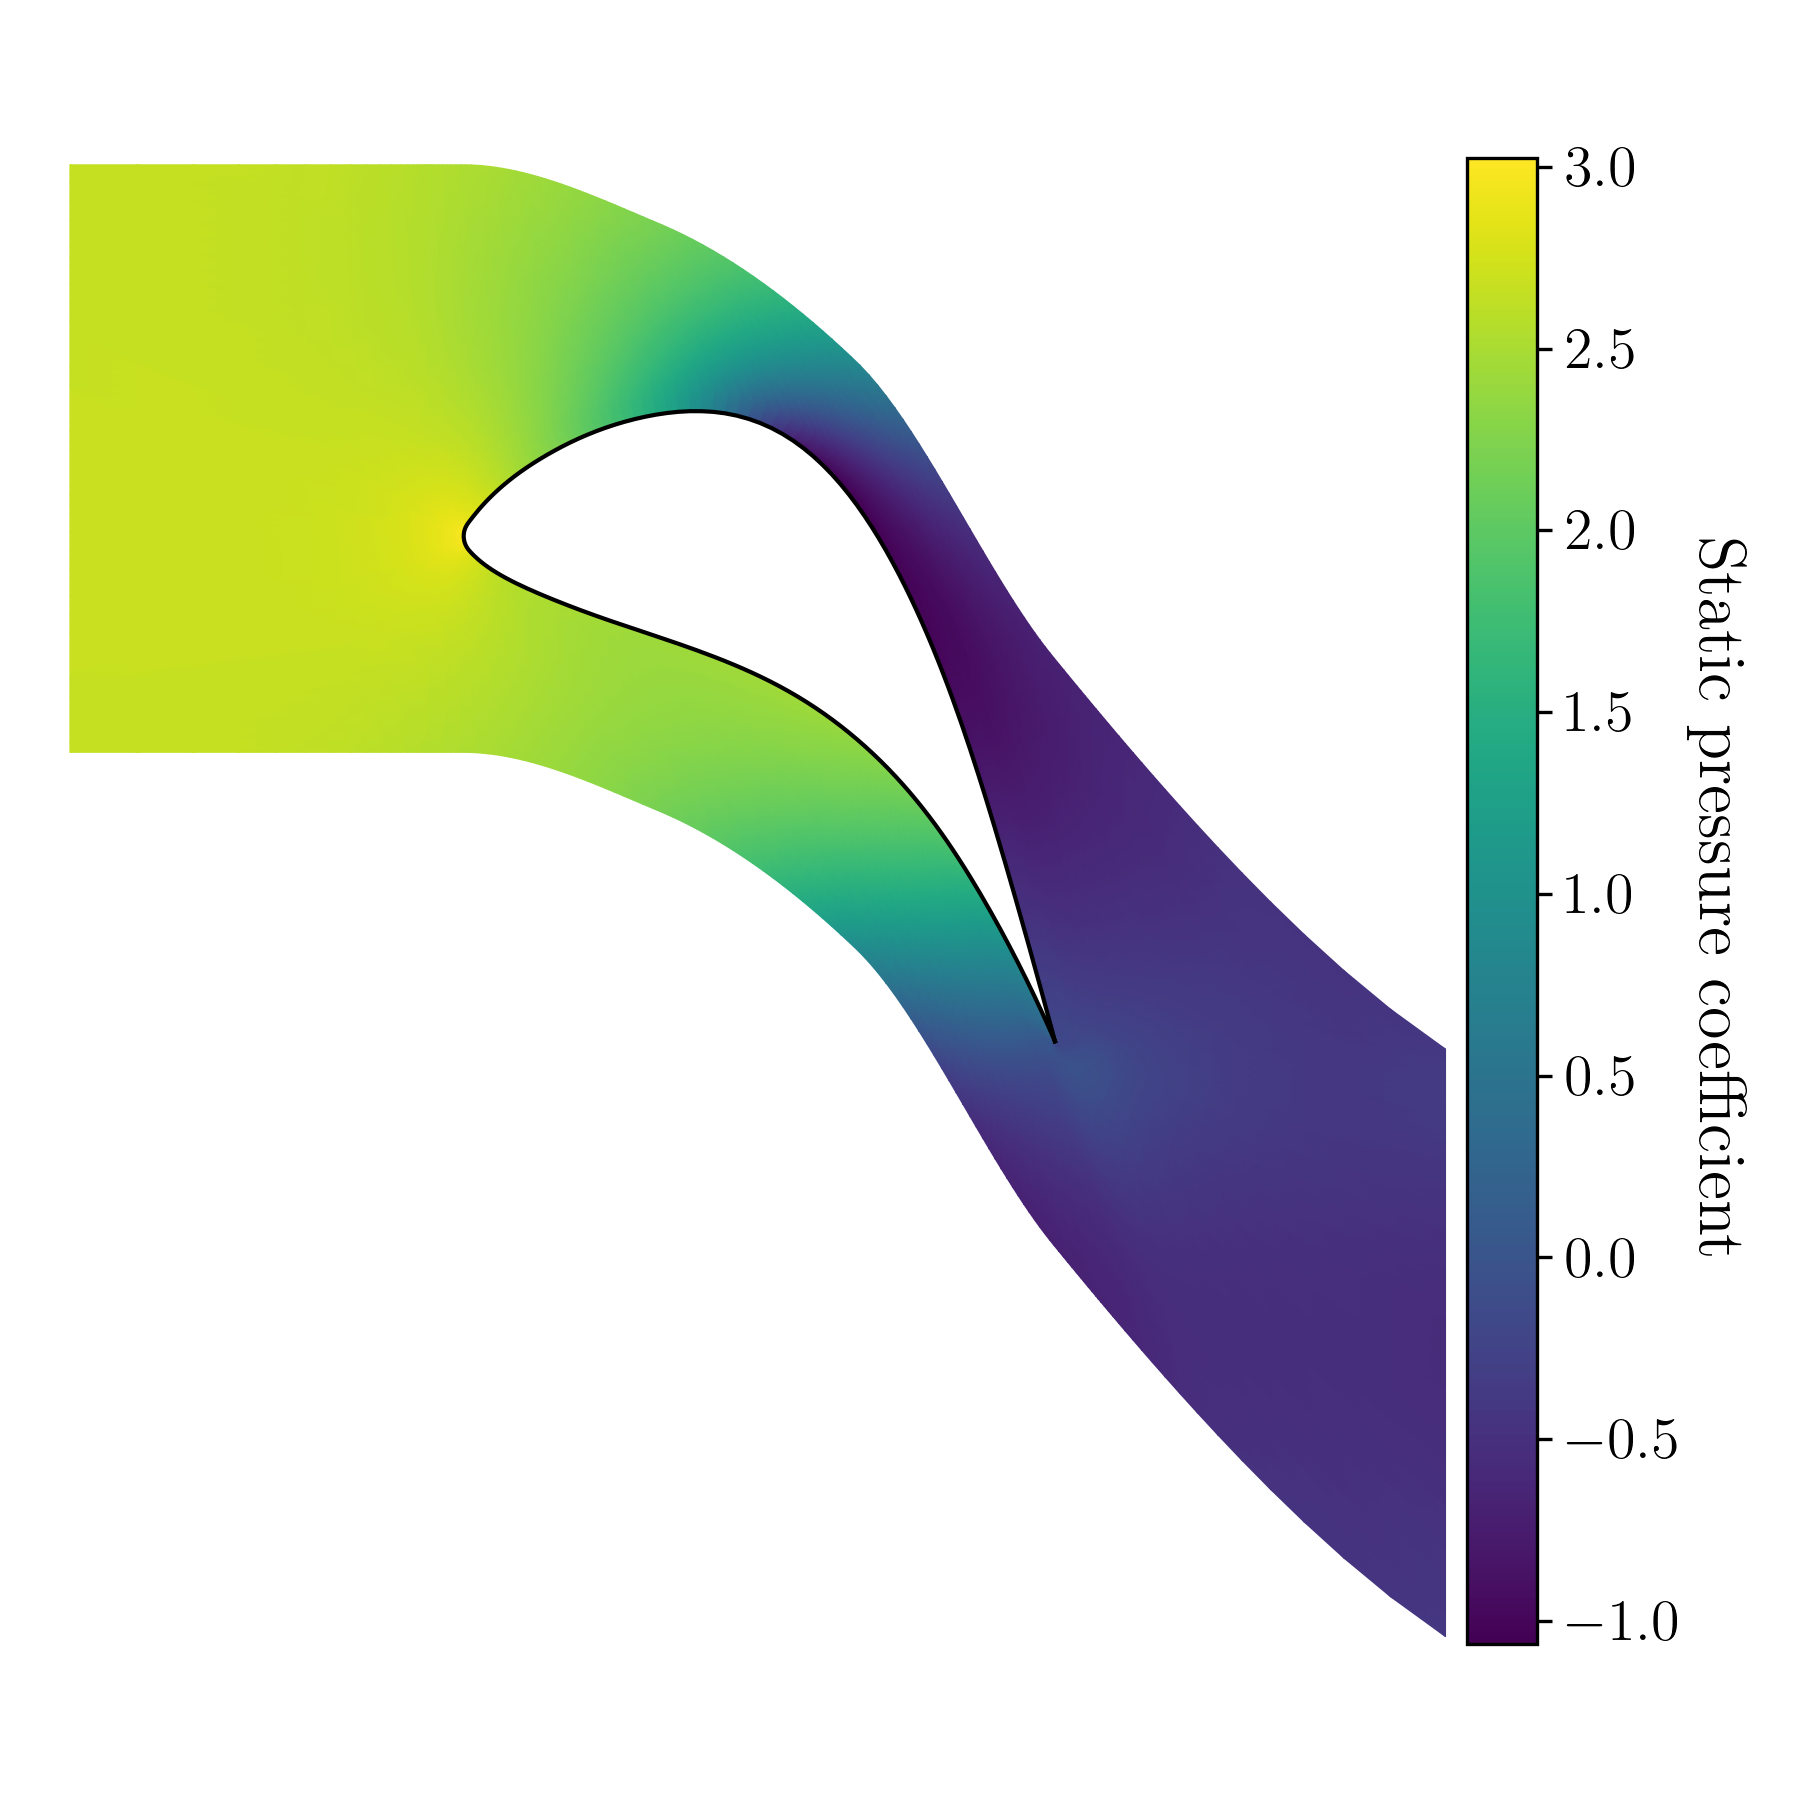
\includegraphics[width=0.99\textwidth]{figures/turbine_c_cp.png}
        \caption{}
        \label{fig:turbine_c_cp}
    \end{subfigure}
    \begin{subfigure}{0.55\textwidth}
        \centering
        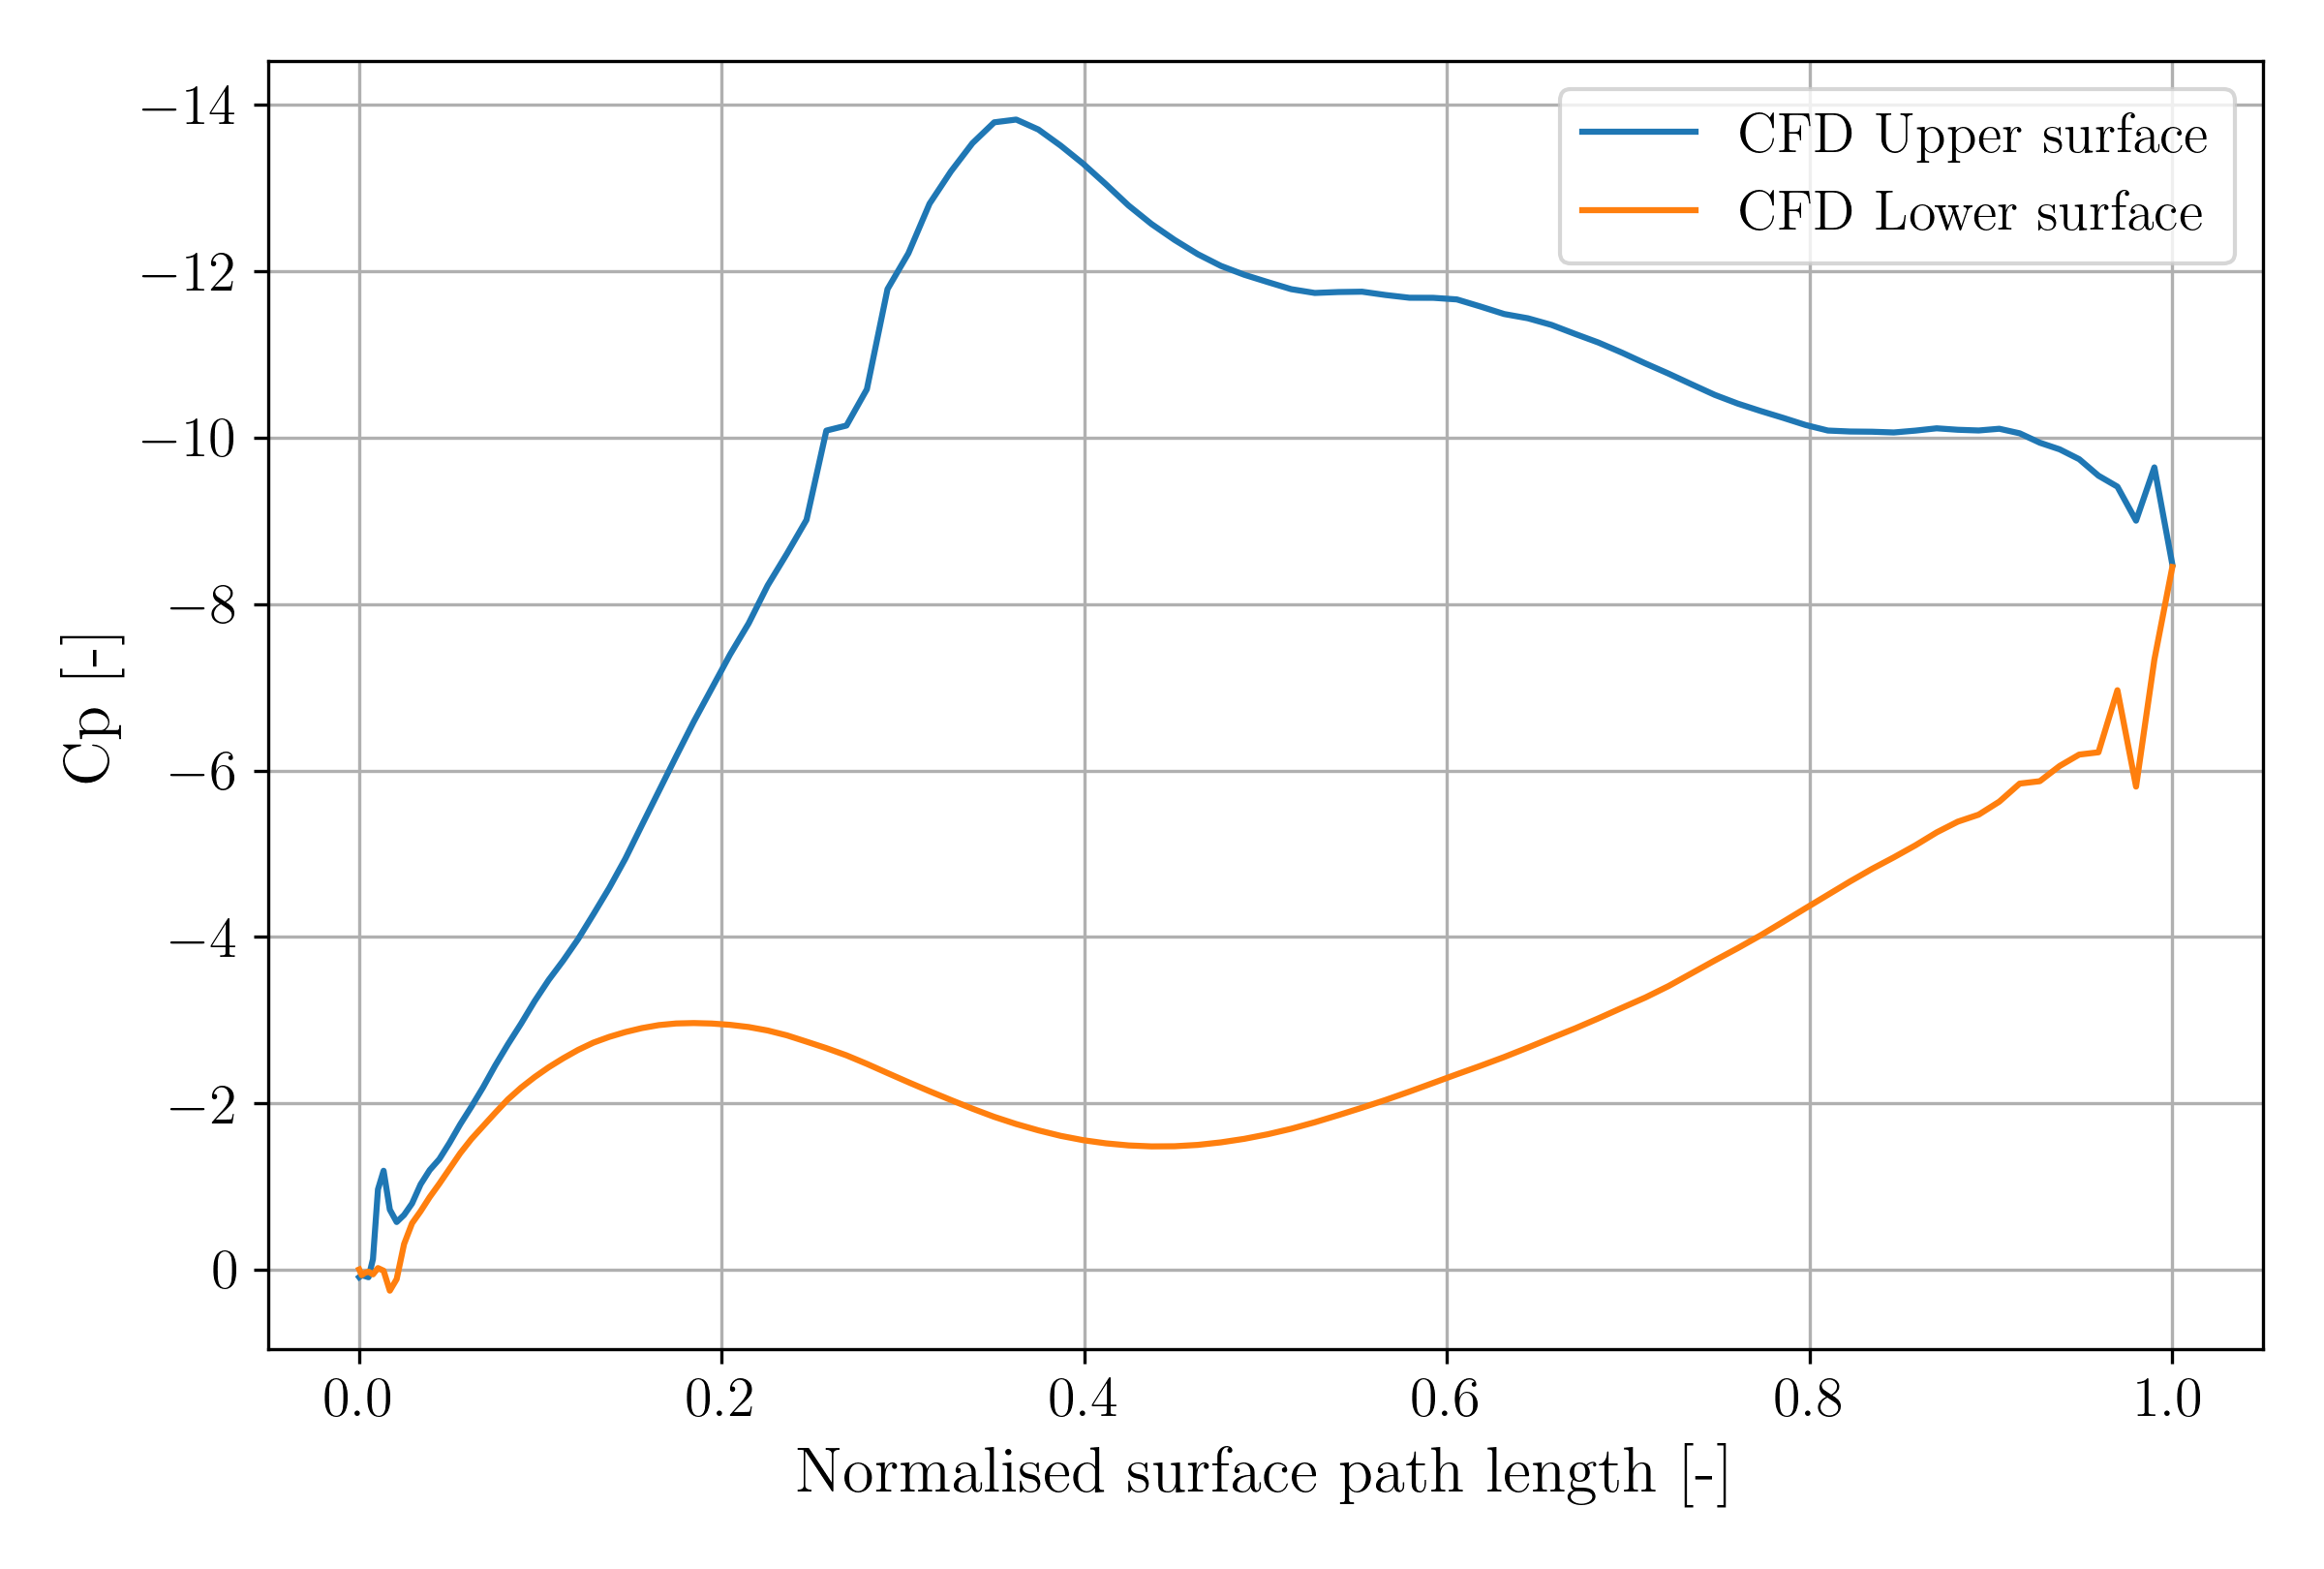
\includegraphics[width=0.99\textwidth]{figures/turbine_c_surface_cp_0.0.png}
        \caption{}
        \label{fig:turbine_c_surface_cp}
    \end{subfigure}
    \caption{Turbine\_c test case results}
\end{figure}

\begin{figure}[H]
    \centering
    \begin{subfigure}{0.44\textwidth}
        \centering
        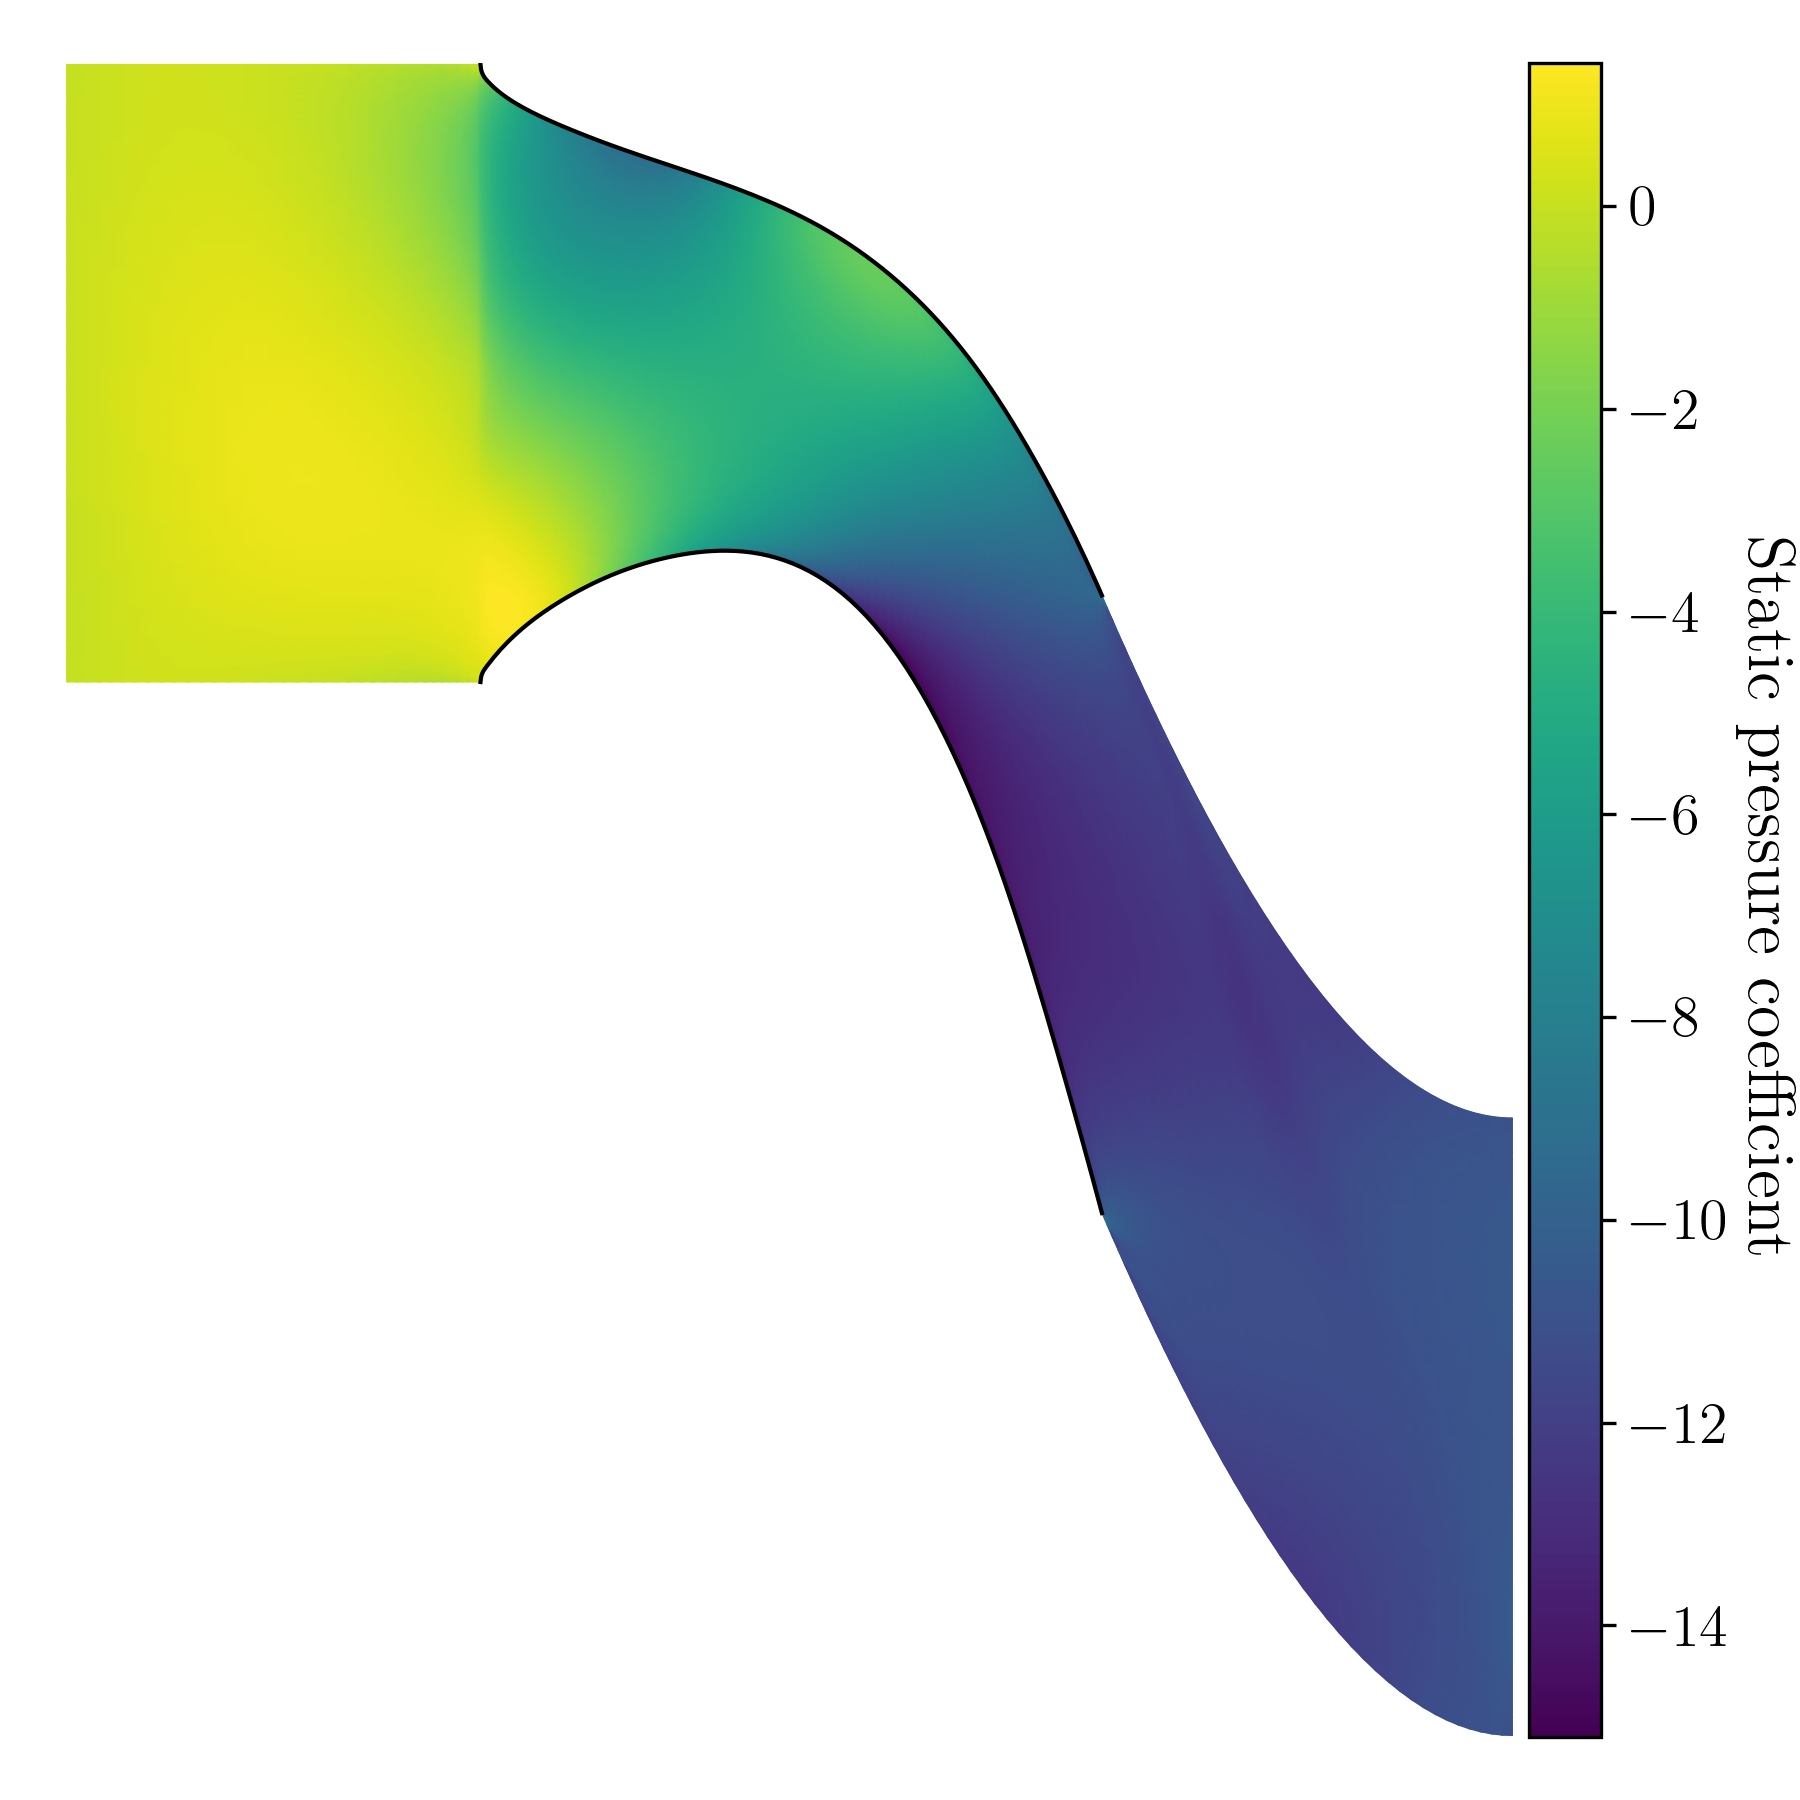
\includegraphics[width=0.99\textwidth]{figures/turbine_h_cp.png}
        \caption{}
        \label{fig:turbine_h_cp}
    \end{subfigure}
    \begin{subfigure}{0.55\textwidth}
        \centering
        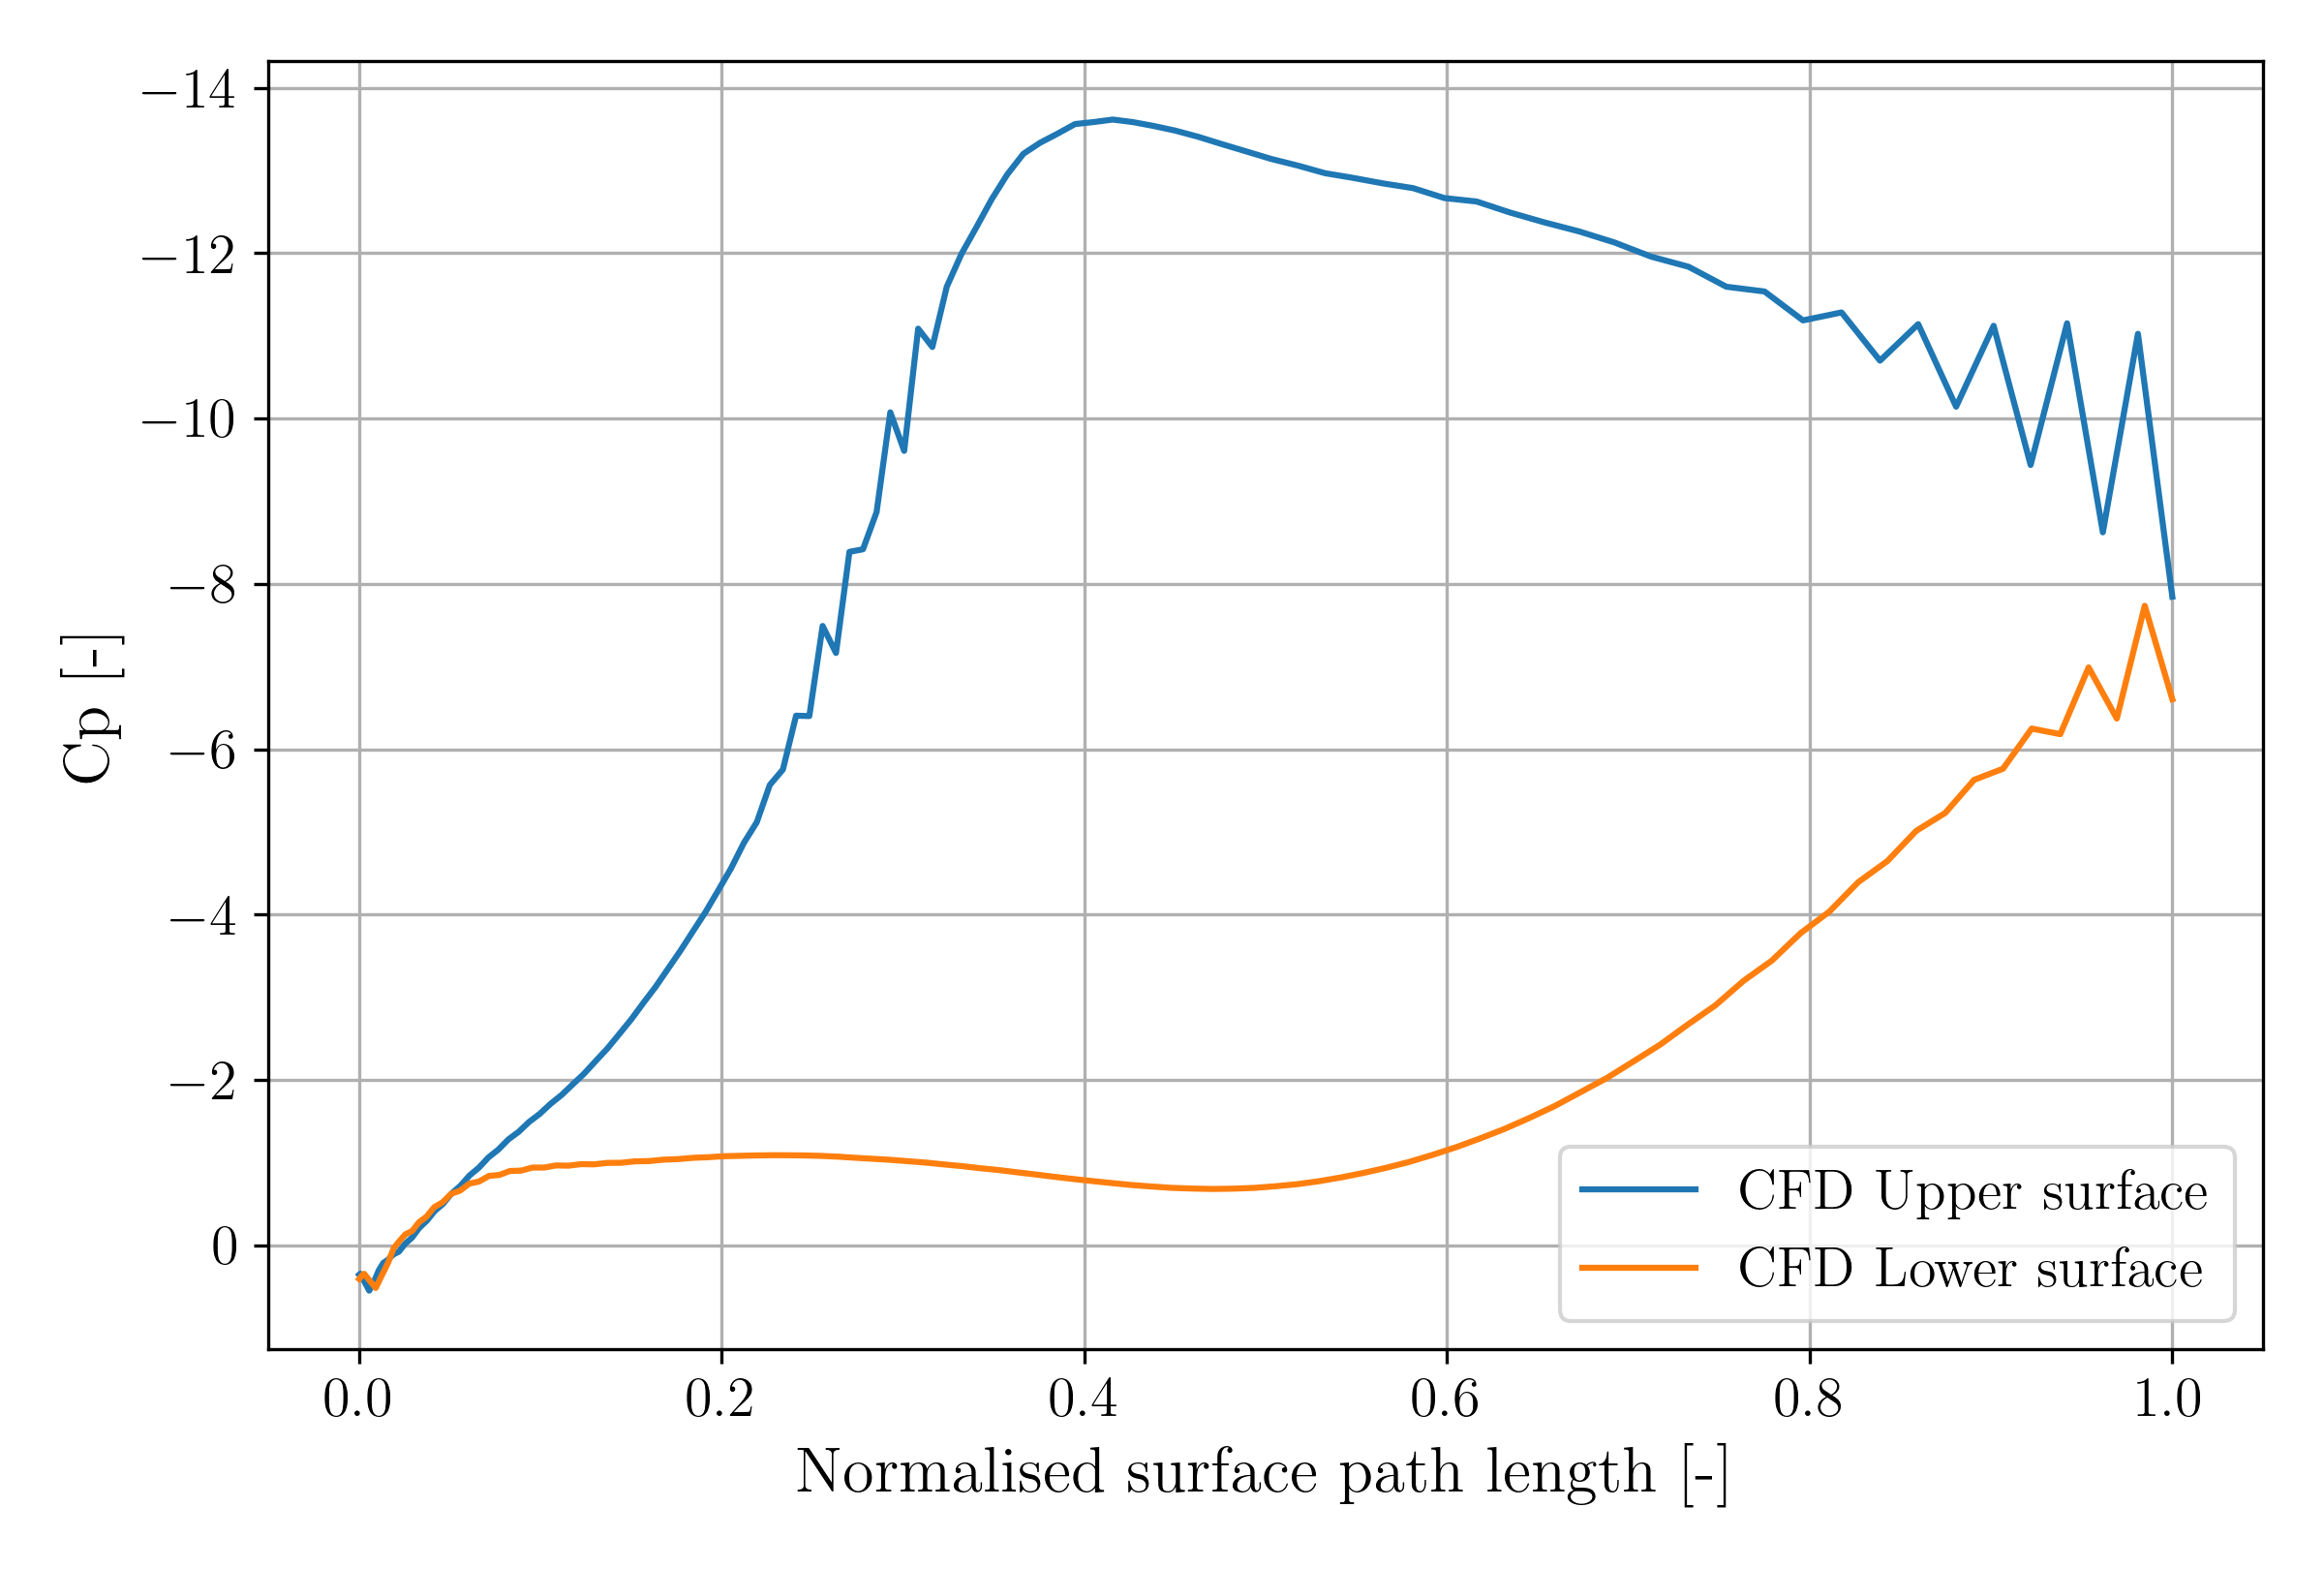
\includegraphics[width=0.99\textwidth]{figures/turbine_h_surface_cp_0.0.png}
        \caption{}
        \label{fig:turbine_h_surface_cp}
    \end{subfigure}
    \caption{Turbine\_h test case results}
\end{figure}

\section{Discussion}
% two pages that doesnt repeat interim

\subsection{Improvements}

Individual improvements were tested to see how they affected the solver.

Figures \ref{fig:improvements_cfl_residual} and \ref{fig:improvements_ni_residual} show the temporal and spatial accuracy of the solver for the various improvements.
The default solver is shown with no improvements and has the same first order temporal and second order spatial accuracy.
It is clear from the gradients that none of the improvements change the order of accuracy of the final steady state solution compared to the default solver.
It can be also seen that deferred correction improves the accuracy which is to be expected from the reduced artificial smoothing.
The same plateau in accuracy is observed for larger meshes due to floating point errors limiting the accuracy of area and spatial derivatives.
Again the deviation is also observed for the smallest mesh sizes which is thought to be due to boundary conditions applied over significant sections of the mesh.
The graphs also show only the converged runs for same logarithmic spacing of \texttt{cfl} and \texttt{ni}.
More missing points indicate instability of the parameters and it can be seen that at high \texttt{cfl} the spatially varying timestep and deferred correction both reduce the stability of the default solver.
The spatially varying timestep clearly reduces the stability as the most unstable cell is being updated by a larger local timestep than the previous smaller global timestep.
The deferred correction cancels out the artificial viscosity and so when run with the same \texttt{sfac} as the default case, the final smoothing is reduced which is shown to reduce stability at high \texttt{cfl} numbers \cite{interim}.

The relation of the runtime to \texttt{cfl} and \texttt{ni} is shown in figures \ref{fig:improvements_cfl_time} and \ref{fig:improvements_ni_time}.
Most of the improvements show the same runtime order as the default $T\sim\mathcal{O}(\texttt{cfl}^{-1/2})$ with the exception of the deferred correction.
The small region shows a runtime inversely proportional to \texttt{cfl}.
This is thought to be due to primary flow variables now being smoothed to an additional term, \texttt{corr}, that itself converges to \texttt{corr\_total}.
This could effectively double the runtime order of the default solver.
The Runge Kutta improvement shows a noticeable increase in runtime at the same \texttt{cfl} which is expected due to the increased number of intermediate timesteps.
This method also increases stability for larger \texttt{cfl} timesteps, allowing faster convergence and reducing the overall runtime.
From figure \ref{fig:improvements_ni_time} the spatial runtime order is the same first order as the default solver for all improvements.
At high \texttt{cfl} numbers and low \texttt{ni}, a plateau in runtime is observed which convergence before the minimum number of iterations to meet the convergence criteria discussed earlier.
This is most apparent for the small mesh sizes where convergence occurs in significantly fewer iterations.


The combination of all the improvements are then tested to see how they affect the solver.

Figure \ref{fig:cfl_sfac_dro_avg} shows the effect of \texttt{cfl} and \texttt{sfac} on the stability and residual error (accuracy) of the solver.
When compared to the same figure for the default solver in the interim report \cite{interim}, the improvement show stability at much higher \texttt{cfl} numbers.
It also shows stability at much lower \texttt{sfac} numbers which is thought to be due to the inclusion of residual averaging.

Figures \ref{fig:effort_vs_accuracy_1} and \ref{fig:effort_vs_accuracy_2} show the final steady state residual plotted against runtime for converged bump cases with varying parameters.
This effectively provides an effort vs accuracy curve for the solver.
The contour lines shown on each graph are the figure of merit (FM) defined in equation \ref{eq:FM}.
Parameters that give the highest FM, or the most accuracy in a given time, or the least time for a given accuracy are the most desirable.

Figure \ref{fig:effort_vs_accuracy_cfl} shows decreasing \texttt{cfl} improves the accuracy which has already been shown however it does so along a constant FM contour.
The size of markers for this graph represents the \texttt{sfac} which shows by reducing this parameter, a significant increases in FM for the same \texttt{cfl} can be achieved.
This cannot be seen for extreme \texttt{cfl} numbers with low numbers taking significant runtime and high numbers being unstable as seen in \ref{fig:cfl_sfac_dro_avg}.
The deviation from constant FM contour at low runtimes may again be due to the solution not meeting convergence criteria when it should.
Low \texttt{sfac} at high \texttt{cfl} numbers have an increased runtime than high \texttt{sfac} which is thought to be due to the increased unstable oscillations
present in convergence history, delaying convergence criteria.

Figure \ref{fig:effort_vs_accuracy_ni} shows the effect of varying the number of cells in the \texttt{i} direction on the effort vs accuracy curve.
Again the same trend as \ref{fig:improvements_ni_residual} is observed where accuracy increases second order and time increases linearly.
The plateau due to floating point precision at high mesh values limit the accuracy that can be gained for an increase in effort.
This gives rise to an \textit{optimal mesh size} where the FM is maximised.
For the bump case this is seen to be around $\texttt{ni}=200$, reaching $FM =4.5$.
The size of markers for this graph represents the \texttt{sfac}.
Groups of same \texttt{ni} can be identified by lines of same colour but decreasing marker sizes.
These lines show that decreasing \texttt{sfac} increases the FM for the same \texttt{ni} and \texttt{cfl}.

Figure \ref{fig:effort_vs_accuracy_fcorr} shows the effect of varying \texttt{fcorr} and \texttt{sfac} on the effort vs accuracy curve.
The size of the markers represents the factor \texttt{fcorr} of artificial viscosity to be cancelled out.
The colour represents the amount of artifical viscosity \texttt{sfac} added to the solution.
The previous trends of reduced \texttt{sfac} increasing accuracy for given effort are observed.
Most importantly, increasing \texttt{fcorr} gives a significant rise in accuracy for a marginal increase in runtime.
This increase in runtime for a fixed \texttt{cfl} is due to the increased final smoothing \texttt{fcorr\_total} that must be reached in the same rate \texttt{corr\_rate} \ref{eq:corr_rate}.
Interestingly, at very low \texttt{sfac} the runtime slightly decreases upon increasing \texttt{fcorr}.
This faster convergence must be due to the reduced smoothing factors towards the end of convergence but its not clear the exact mechanism that causes this.

The final plot, figure \ref{fig:effort_vs_accuracy_sfac_res} shows the effect of varying \texttt{sfac\_res} and \texttt{cfl} on the effort vs accuracy curve.
The colour is $\log_{10}(\texttt{cfl})$ and the size is \texttt{sfac\_res}.
The graph shows that increasing the residual averaging factor \texttt{sfac\_res} for modest to low \texttt{cfl} numbers, increases the runtime with similar accuracy.
Small markers are missing at high \texttt{cfl} numbers which demonstrates the increased stability of residual averaging.
However, these increased timesteps have poor accuracy and high runtime and so dont have a high FM.
The small runtimes are likely to be innacurate however, as the solution is converging well before meeting the convergence criteria.

\subsection{NACA airfoils}

Multigrid arrangements can be used to solve the Euler equations for external flows.
NACA airfoil flow results are compared to panel method solutions from the SA1 report \cite{SA1}.
Typical panel methods explicitly apply the Kutta condition at the trailing edge to ensure the flow leaves smoothly.
This is not necessary for the Euler solver as the artificial viscosity of the solver is enough to make the flow leave the trailing edge smoothly.
The panel method includes a boundary layer solver but this is uncoupled from the invicid flow solvler and so the $C_p$ results can be compared directly.
The Reynolds number is matched to the dynamic pressure boundary condition at an altitude of 35000ft.
For 15kPa dynamic pressure this corresponds to a Reynolds number of $\sim7\times10^6$.

Figure \ref{fig:naca0012_cp} shows the pressure coefficient of the computational domain for the NACA0012 airfoil at $\alpha = 0^\circ$.
As expected the flow is highly symmetrical with pressure coefficient of 0 in the far field. The stagnation point is observed at the leading edge with a pressure coefficient of 1.
The flow is then accelerated faster than freestream flow over upper and lower surfaces before rejoining at the trailing edge.
Figure \ref{fig:naca0012_surface_cp} shows the pressure coefficient on the surface of the NACA0012 airfoil at $\alpha = 0^\circ$.
The y axis is flipped so that the suction surface line is at the top of the graph.
The upper and lower pressure coefficient lines are exactly on top of eachother, which is expected for a symmetric airfoil.
There is a slight discrepancy between the upper and lower surfaces, the suction peak predicted by CFD is marginally higher and further back.
This is likely due to numerical accuracy or a single index difference in the plotting function.
The NACA2412 airfoil is shown in figure \ref{fig:naca2412_cp} and \ref{fig:naca2412_surface_cp} at $\alpha = 0^\circ$.
A stronger suction peak is observed on the top surface which is to be expected for a cambered airfoil.
The $C_p$ curves are also in strong agreement with the SA1 panel method results.
The upper surface of the CFD solution is again slightly higher and further back than the panel method solution.
Figures \ref{fig:naca0012_surface_cp} and \ref{fig:naca2412_surface_cp} both have a discontinous trailing edge which where the artifical smoothing 
is working to apply the Kutta condition. This can be seen more clearly on the residual map in figure \ref{fig:kutta}.

Figure \ref{fig:cl_alpha} shows the lift coefficient against angle of attack for the NACA0012 and NACA2412 airfoils.
The graph shows strong linear relationship for nearly all angles of attack.
From invicid theory, these lift coefficient should be linear with angle of attack with gradient $ 2\pi $.
However the gradient is observed to be ~0.3, significantly smaller than the theoretical value.
Plots of the panel method solution show a gradient of $2\pi$. The NACA2412 case intersects $\alpha = 0$ at a lift coefficient 25.8\% higher than the CFD solution shown in figure \ref{fig:naca2412_surface_cp}.
The drag coefficient can also be calculated from the pressure coefficients, which for the invicid solver should be zero.
These are shown in figure \ref{fig:cd_alpha} and show a similar linear relationship, both intersecting close to 0,0.
% TODO: 
% discuss Kutta condition 
% not necessary to explicitly apply 
% because the artificial viscosity of the solver is enough to make the flow leave the trailing edge smoothly

Figure \ref{fig:naca0012_cp5} and \ref{fig:naca0012_surface_cp5} show the pressure coefficient map and the surface of the NACA0012 airfoil at $\alpha = 5^\circ$.
Clearly this is very different from the panel method solution.
The reason for this is thought to be due to poorly posed boundary conditions on the domain.
The current method of defining $\alpha$ at a single inlet plane is insufficient for external flow fields.
For a positive $\alpha$ a small amount of flow must enter through the bottom of the domain and leave through the top, which should be possible as these are not set as walls.
However, the problem is better defined by explicitly setting far field boundary conditions.
This may explain why the correct lift and drag coefficients are only observed at $\alpha = 0^\circ$.
Figure \ref{fig:corners} shows the location of the maximum residuals at the corner caused by the discontinous boundary conditions.

\subsection{Turbine}

Theres two turbine cases, turbine\_c and turbine\_h which represent the same stage geometry with the same number of nodes but different mesh topologies.
The geometry is based on a real turbine experiment \cite{4A3_lab} and the pressure inputs shown in shown in table \ref{tab:default_params} are set to values measured from the experiment. 

The results shown in figures \ref{fig:turbine_c_cp} and \ref{fig:turbine_h_cp} show the pressure coefficient in the domain and on the surface of the blade.
The surface pressure distribution shows the characteristic suction peak and adverse pressure gradient to the trailing edge.
However, when compared to real data in figure \ref{fig:turbine_real} the suction peak occurs much earlier and is more pronounced.
Additionally, the real data shows no region of adverse pressure gradient on the bottom surface, which is observed in the CFD solution.

The simpler mesh topology case turbine\_h proved highly unstable, however the results obtained agree more closely with the real data than the turbine\_c case.
Figure \ref{fig:turbine_h_surface_cp} shows a later suction peak and a more gradual adverse pressure gradient on the top surface.
The bottom surface shows a more gradual pressure gradient, still slightly adverse.
However, for this case the trailing edge shows increased oscillations in the pressure coefficient.
This is due to difficulties in applying the Kutta condition accross the averaged patch connecting top and bottom boundaries.
This is likely the reason this simpler geometry is more unstable than the more complex turbine\_c case.

\subsection{Improvements and limitations}
\begin{itemize}
    \item The solver negelcts viscous effects which are important for boundary layers, flow separation and hence lift and drag.
    \item 2D geometry cannot capture 3D flow physics such as tip vorticies or spanwise variations which are particularly important for turbines.
    \item Artificial viscosity can smooth fine scale flow features in shocks or sudden Prantl Meyer expansions.
    \item The spatially varying timestep improvement is only valid for steady state solutions and so cannot capture transient effects.
    \item The convergence criteria means that some cases can converge before the minimum number of iterations to trigger the convergence criteria, giving an innacurate runtime.
    \item The boundary conditions for external flow fields are poorly posed and so at non-zero angles of attack the solver converges to an incorrect solution.
    \item While the solver supports multigrid cases, its scalability and parallelisation for larger, more complex domains were not addressed.
\end{itemize}

\section{Summary}

A 2D Euler solver was developed and tested on a variety of cases.
The solver was improved upon from the interim report by adding Runge-Kutta, deferred correction, residual averaging and spatially varying timestep methods.
Tests revealed significant stability and efficiency gains from the implemented improvements, particularly at higher \texttt{sfac} and \texttt{fcorr}.
A figure of merit was defined to balance improvements in accuracy to increases in runtime.
An optimal mesh size was identified before the limits of floating point precision.
The solver was compared to panel method results for NACA airfoils and showed good agreement at $\alpha = 0^\circ$.
At non-zero angles of attack the solver converged to incorrect solutions which is thought to be due to poorly posed external flow boundary conditions.
Further limitations of the solver were discussed including the neglect of viscous effects, 2D geometry, artificial viscosity and convergence criteria.

Some difficulties involved string and pointer manipulation in Fortran, interoperability between fortran and C++, and debugging strange memory errors.
The development process would benefit significantly from a test driven approach, where functions can be validated at each stage, rather than waiting until halfway through the term to test the entire solver.

\begin{thebibliography}{9}

    \bibitem{handout}
    J. V. Taylor
    \emph{4A2 Computational Fluid Dynamics: Writing an Euler Solver}
    University of Cambridge,
    2024.

    \bibitem{solve_ODE_nonstiff}
    Hairer, Ernst et al.
    \emph{Solving ordinary differential equations I: Nonstiff problems, Berlin, New York}
    Springer-Verlag, Berlin, 1993

    \bibitem{interim}
    L. Pender
    \emph{4A2 Interim Report}
    University of Cambridge,
    2024.

    \bibitem{4A3_lab}
    L. Pender
    \emph{4A3 Turbomachinary Laboratory Report}
    University of Cambridge,
    2024.

    \bibitem{SA1}
    L. Pender
    \emph{SA1 Aircraft Wing Analysis}
    University of Cambridge,
    2024.
  
\end{thebibliography}

\section{Appendix}

\subsection{Software}

\begin{figure}[H]
    \centering
    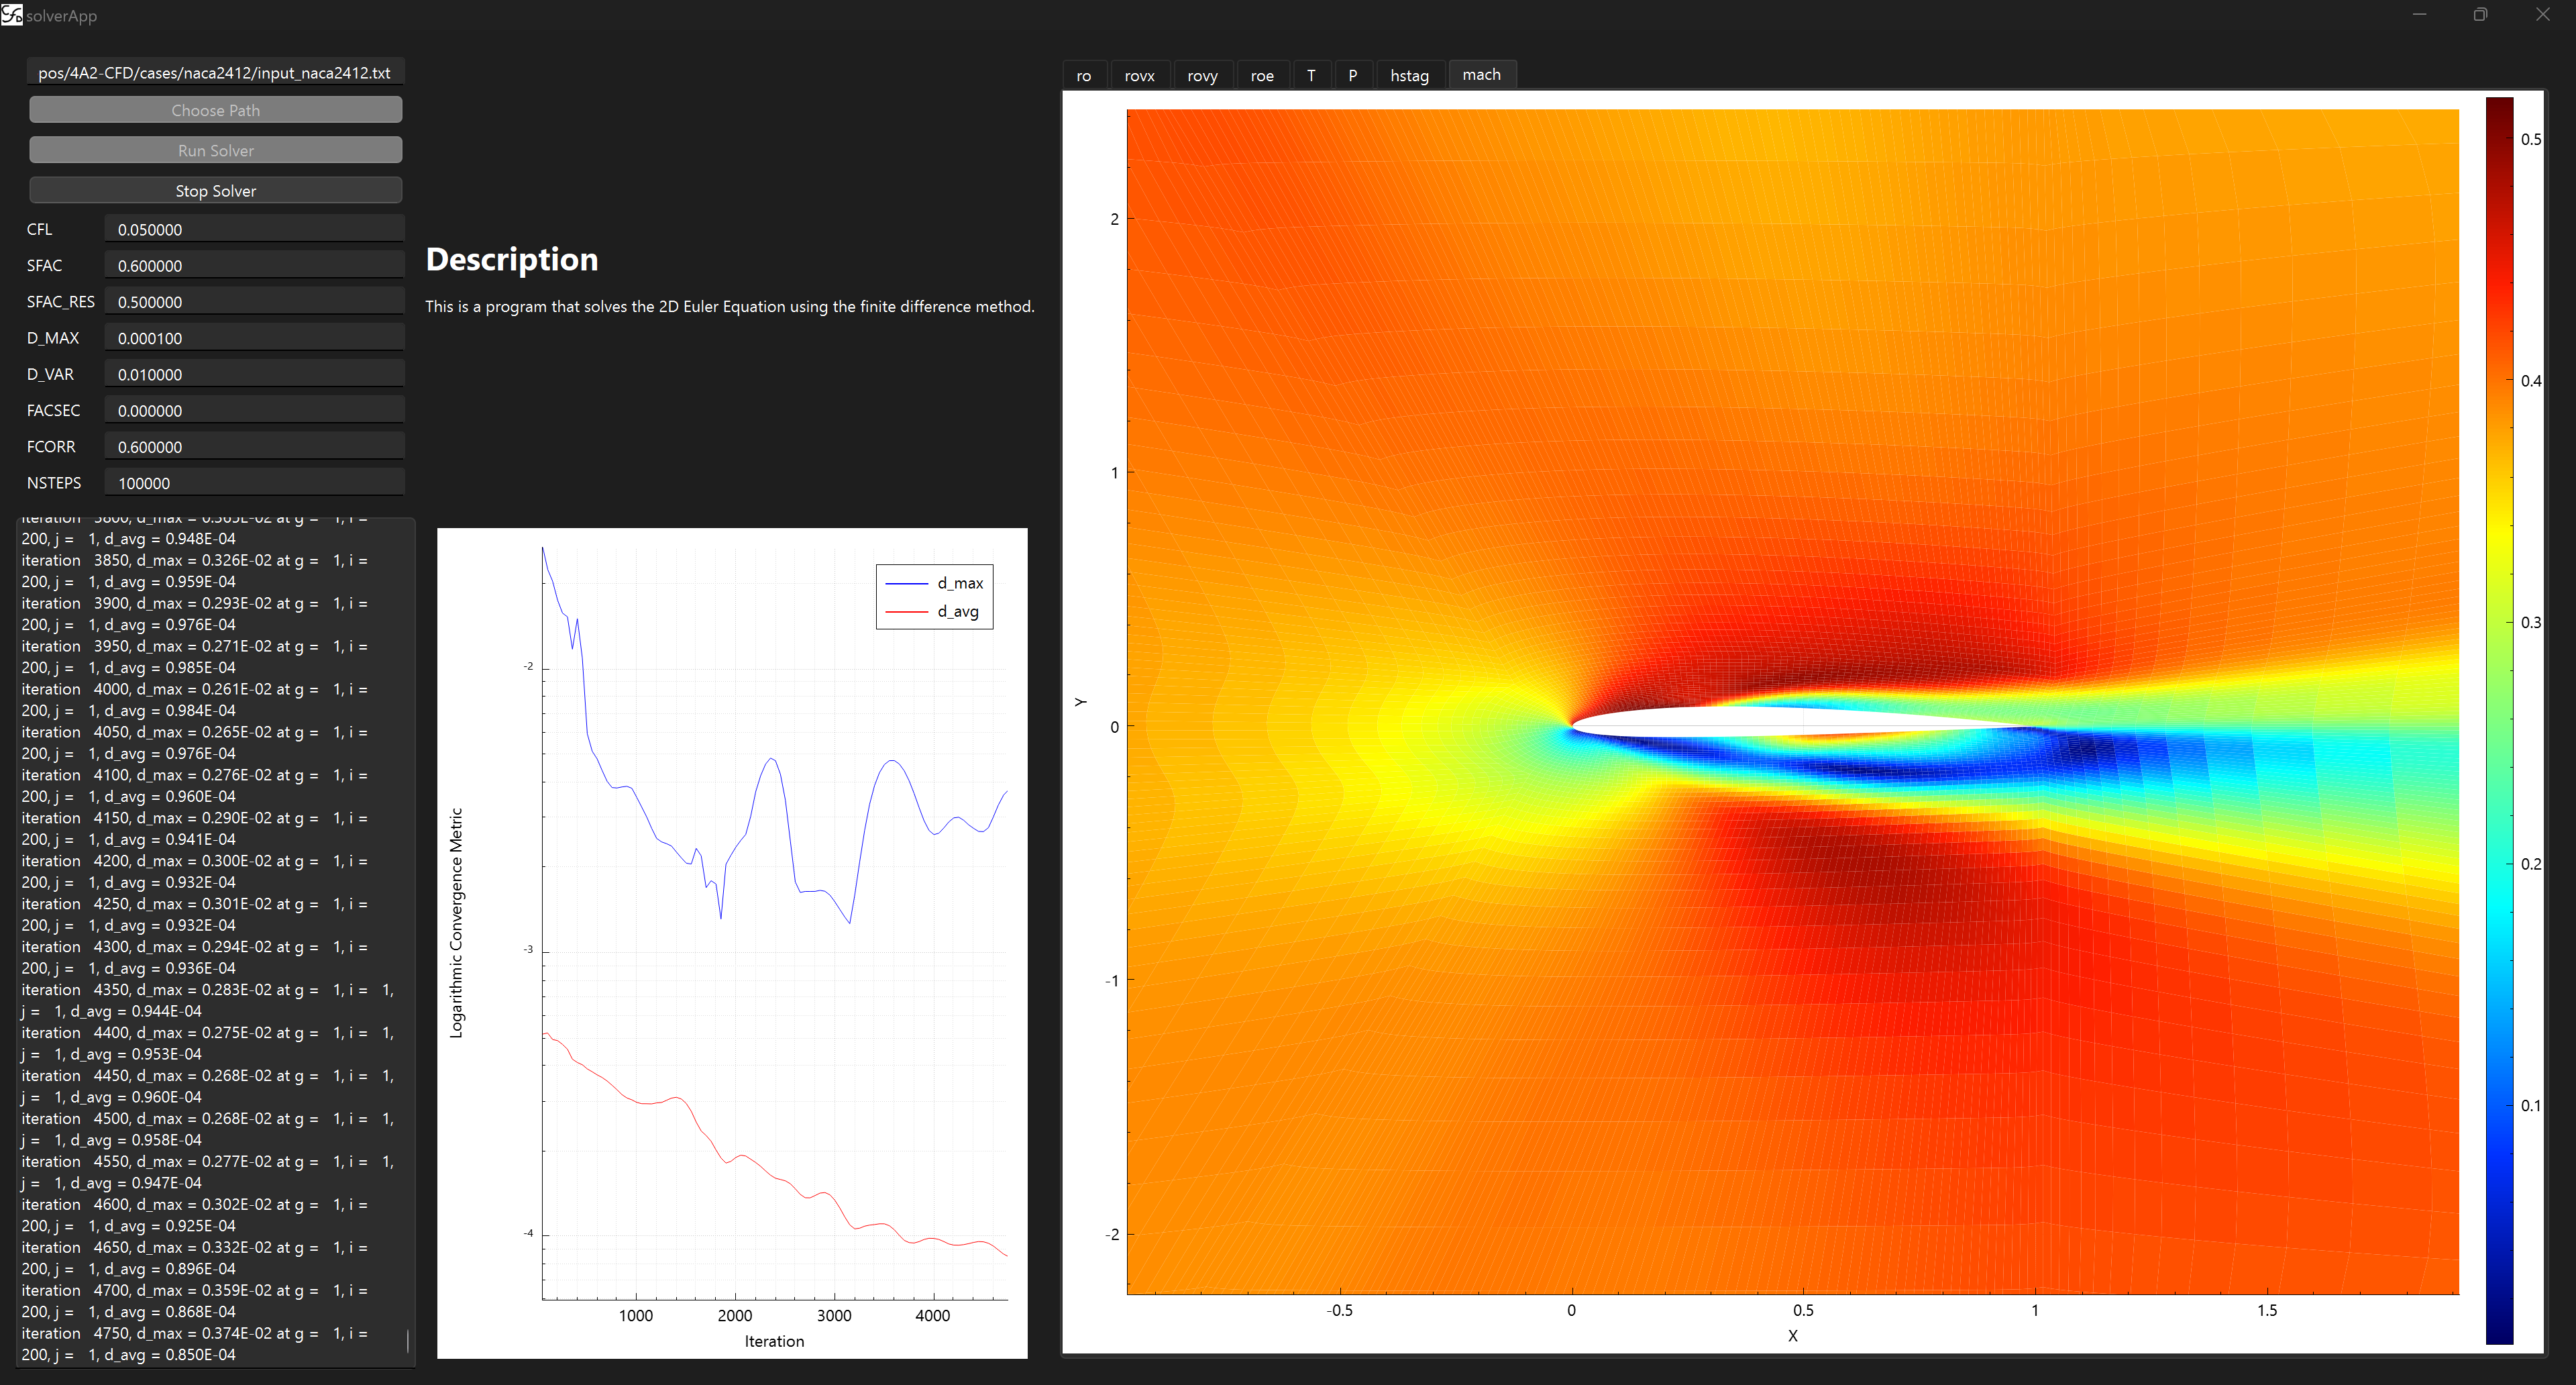
\includegraphics[width=0.7\textwidth]{figures/software.png}
    \caption{Software GUI with inputs, convergance graph and interactive animation tabs}
    \label{fig:software}
\end{figure}

\subsection{Worker runtime enviroment}

A worker directory folder is created in the following format:
% directory tree for bump worker
\begin{figure}[H]
    \dirtree{%
    .1 1.
    .2 bump.
    .3 input\_bump.txt.
    .3 conv\_bump.csv.
    .3 out\_coord\_bump.bin.
    .3 out\_final\_bump.bin.
    .3 geom\_bump.txt.
    .3 out\_guess\_bump.bin.
    .2 log.txt.
    }
    \caption{Worker directory structure}
    \label{fig:worker_dir}
\end{figure}

During setup \texttt{generate\_case} is called and the settings and geometry files are written to the case folder.
During runtime the \texttt{log.txt} acts as \texttt{stdout} for the program.
When the solver finishes then the out files are saved and processed using the postprocessing python functions.

\iffalse
\begin{lstlisting}[language=Python]
def run(self):
    self.setup_environment()
    with open(self.log_file, "w") as log:
        try:
            parsed_file = str(self.in_file).replace("\\", "/")
            t1 = time.time()
            subprocess.run([self.cfd_executable, "--path", parsed_file],
                            check=True,
                            stdout=log)
            t2 = time.time()
        except subprocess.CalledProcessError as e:
            print(f"Worker {self.worker_id} failed with error: {e}")
            return

    self.dt = t2 - t1
    results = self.parse_results()

    # Write results to the shared file in a thread-safe way
    with self.shared_lock:
        with open(self.shared_file, "a", newline="") as csvfile:
            writer = csv.writer(csvfile)
            writer.writerow(results)

    print(f"Worker {self.worker_id} finished.")
\end{lstlisting}
\fi

\subsection{Real turbine comparison}

\iffalse
\begin{figure}[H]
    \centering
    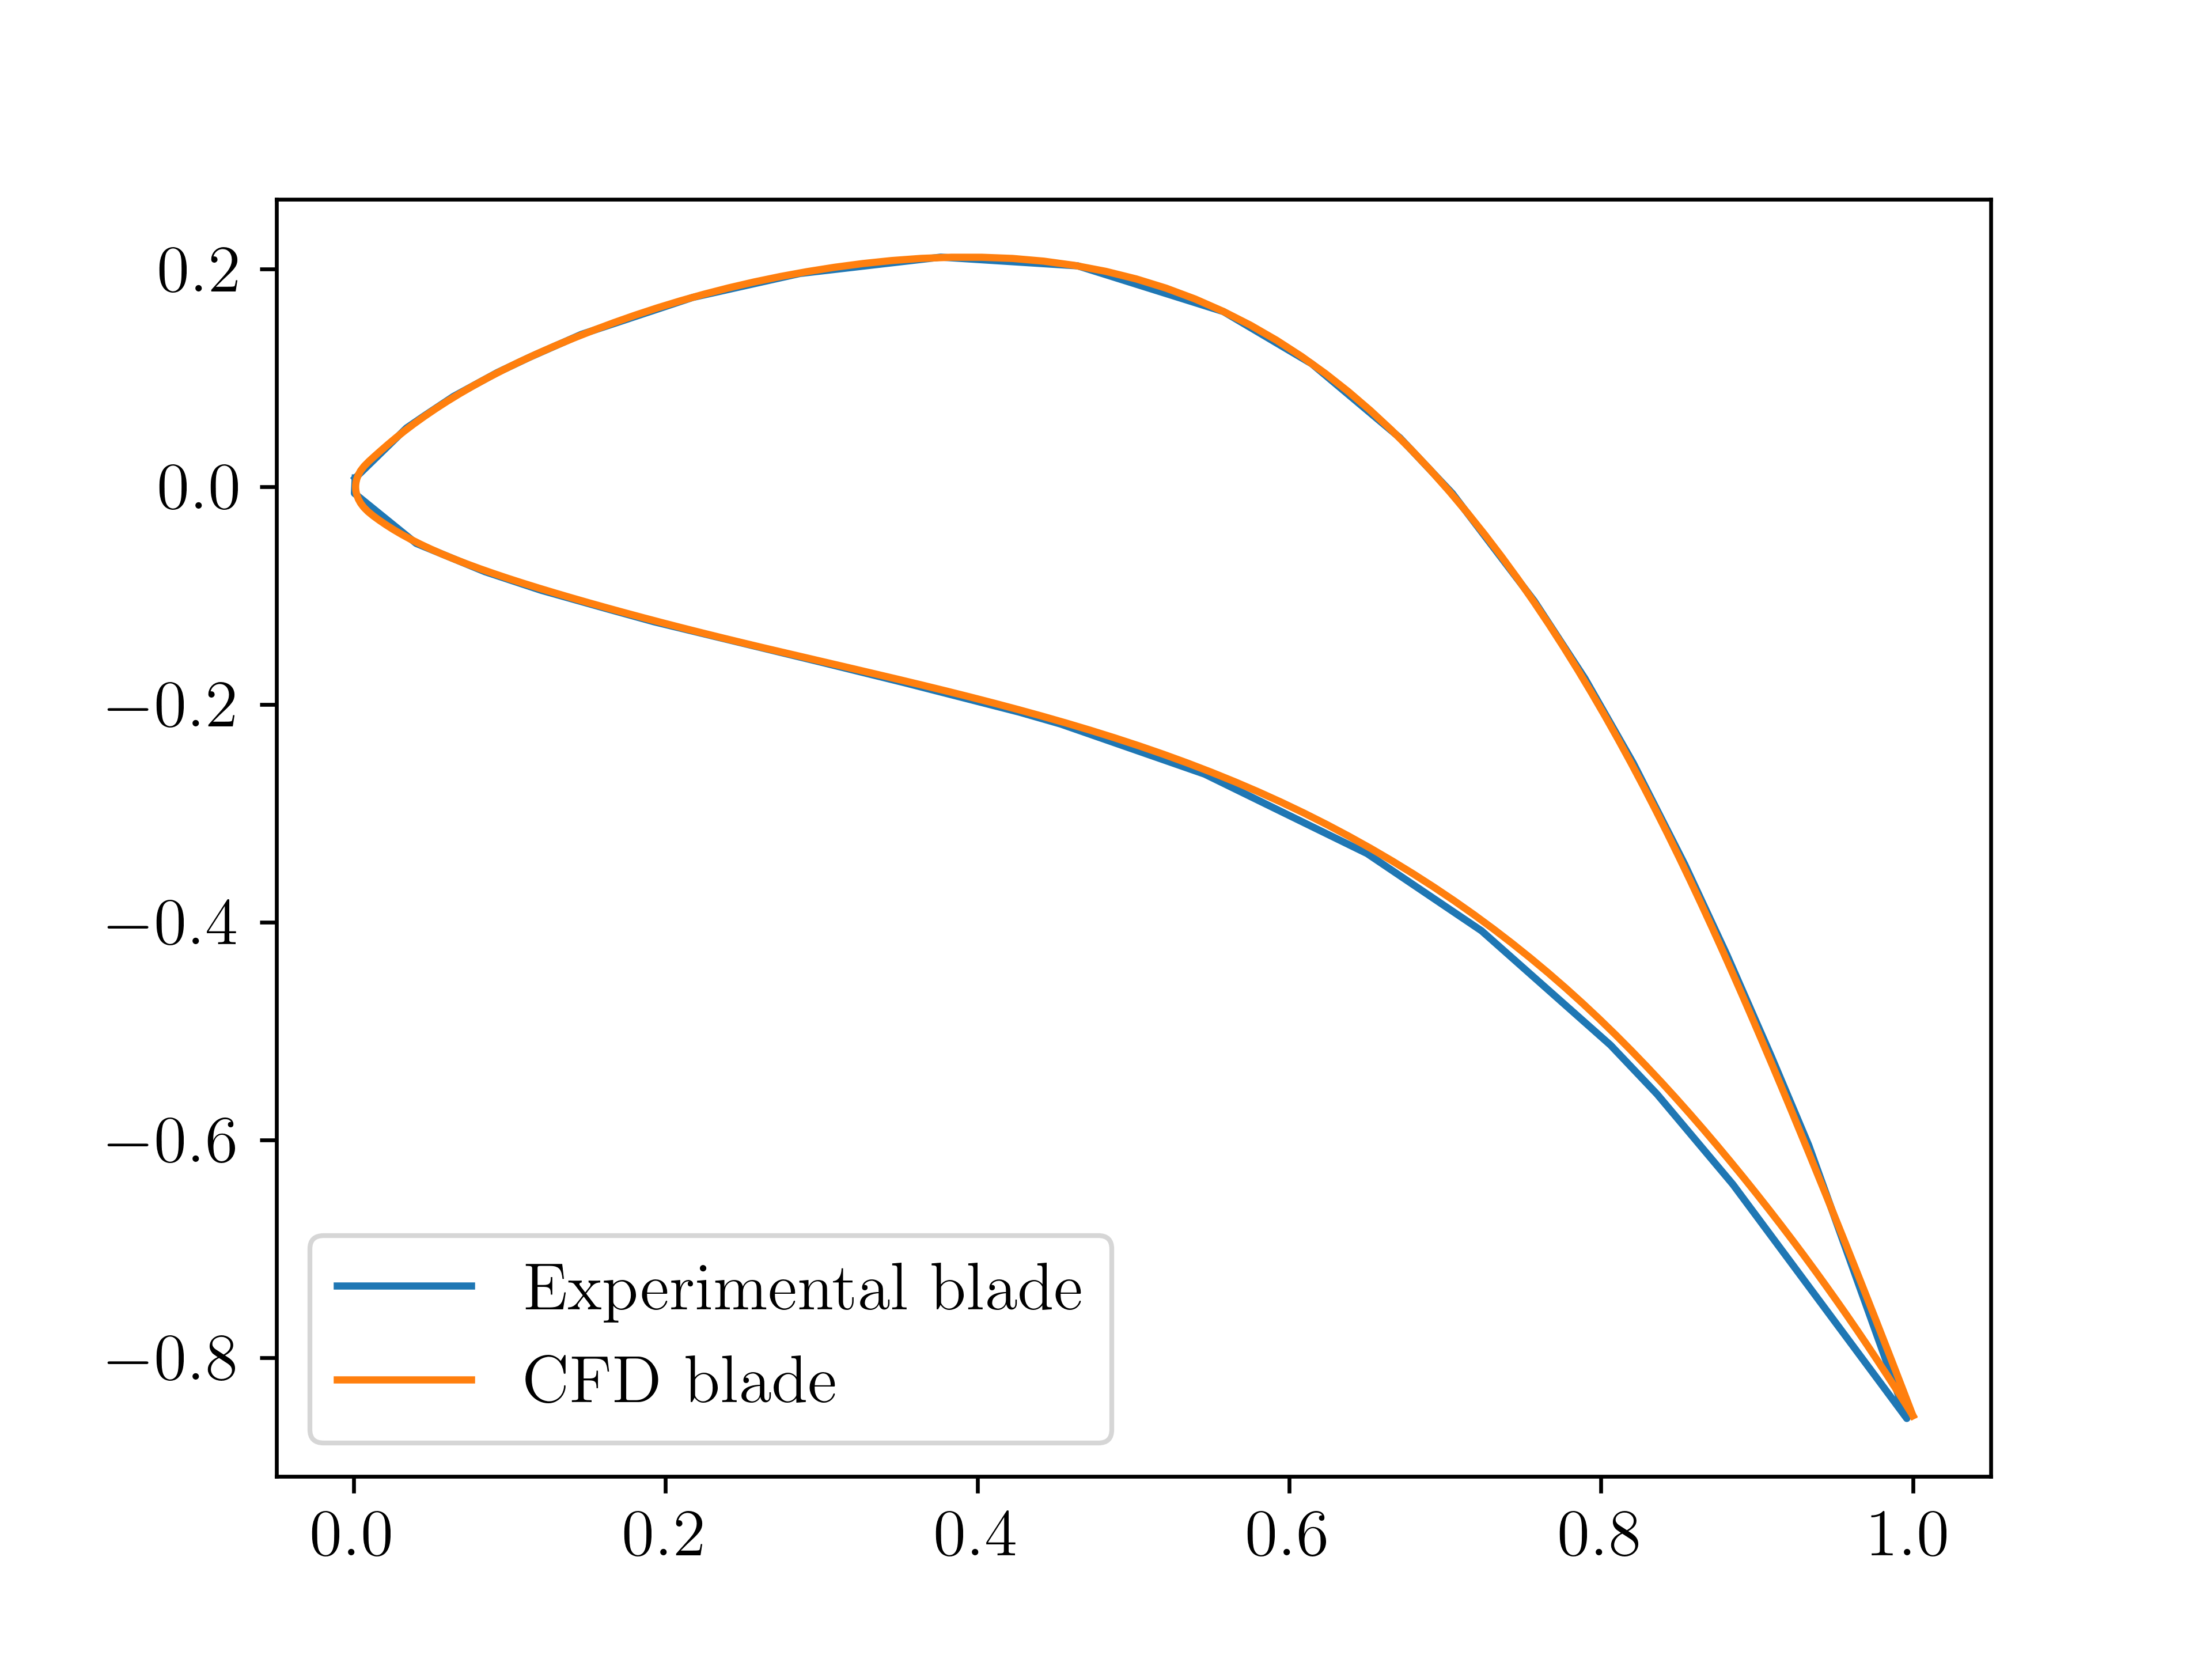
\includegraphics[width=0.6\textwidth]{figures/turbine_geometry.png}
    \caption{Comparison of turbine geometry}
    \label{fig:turbine_geometry}
\end{figure}
\fi

\begin{figure}[H]
    \centering
    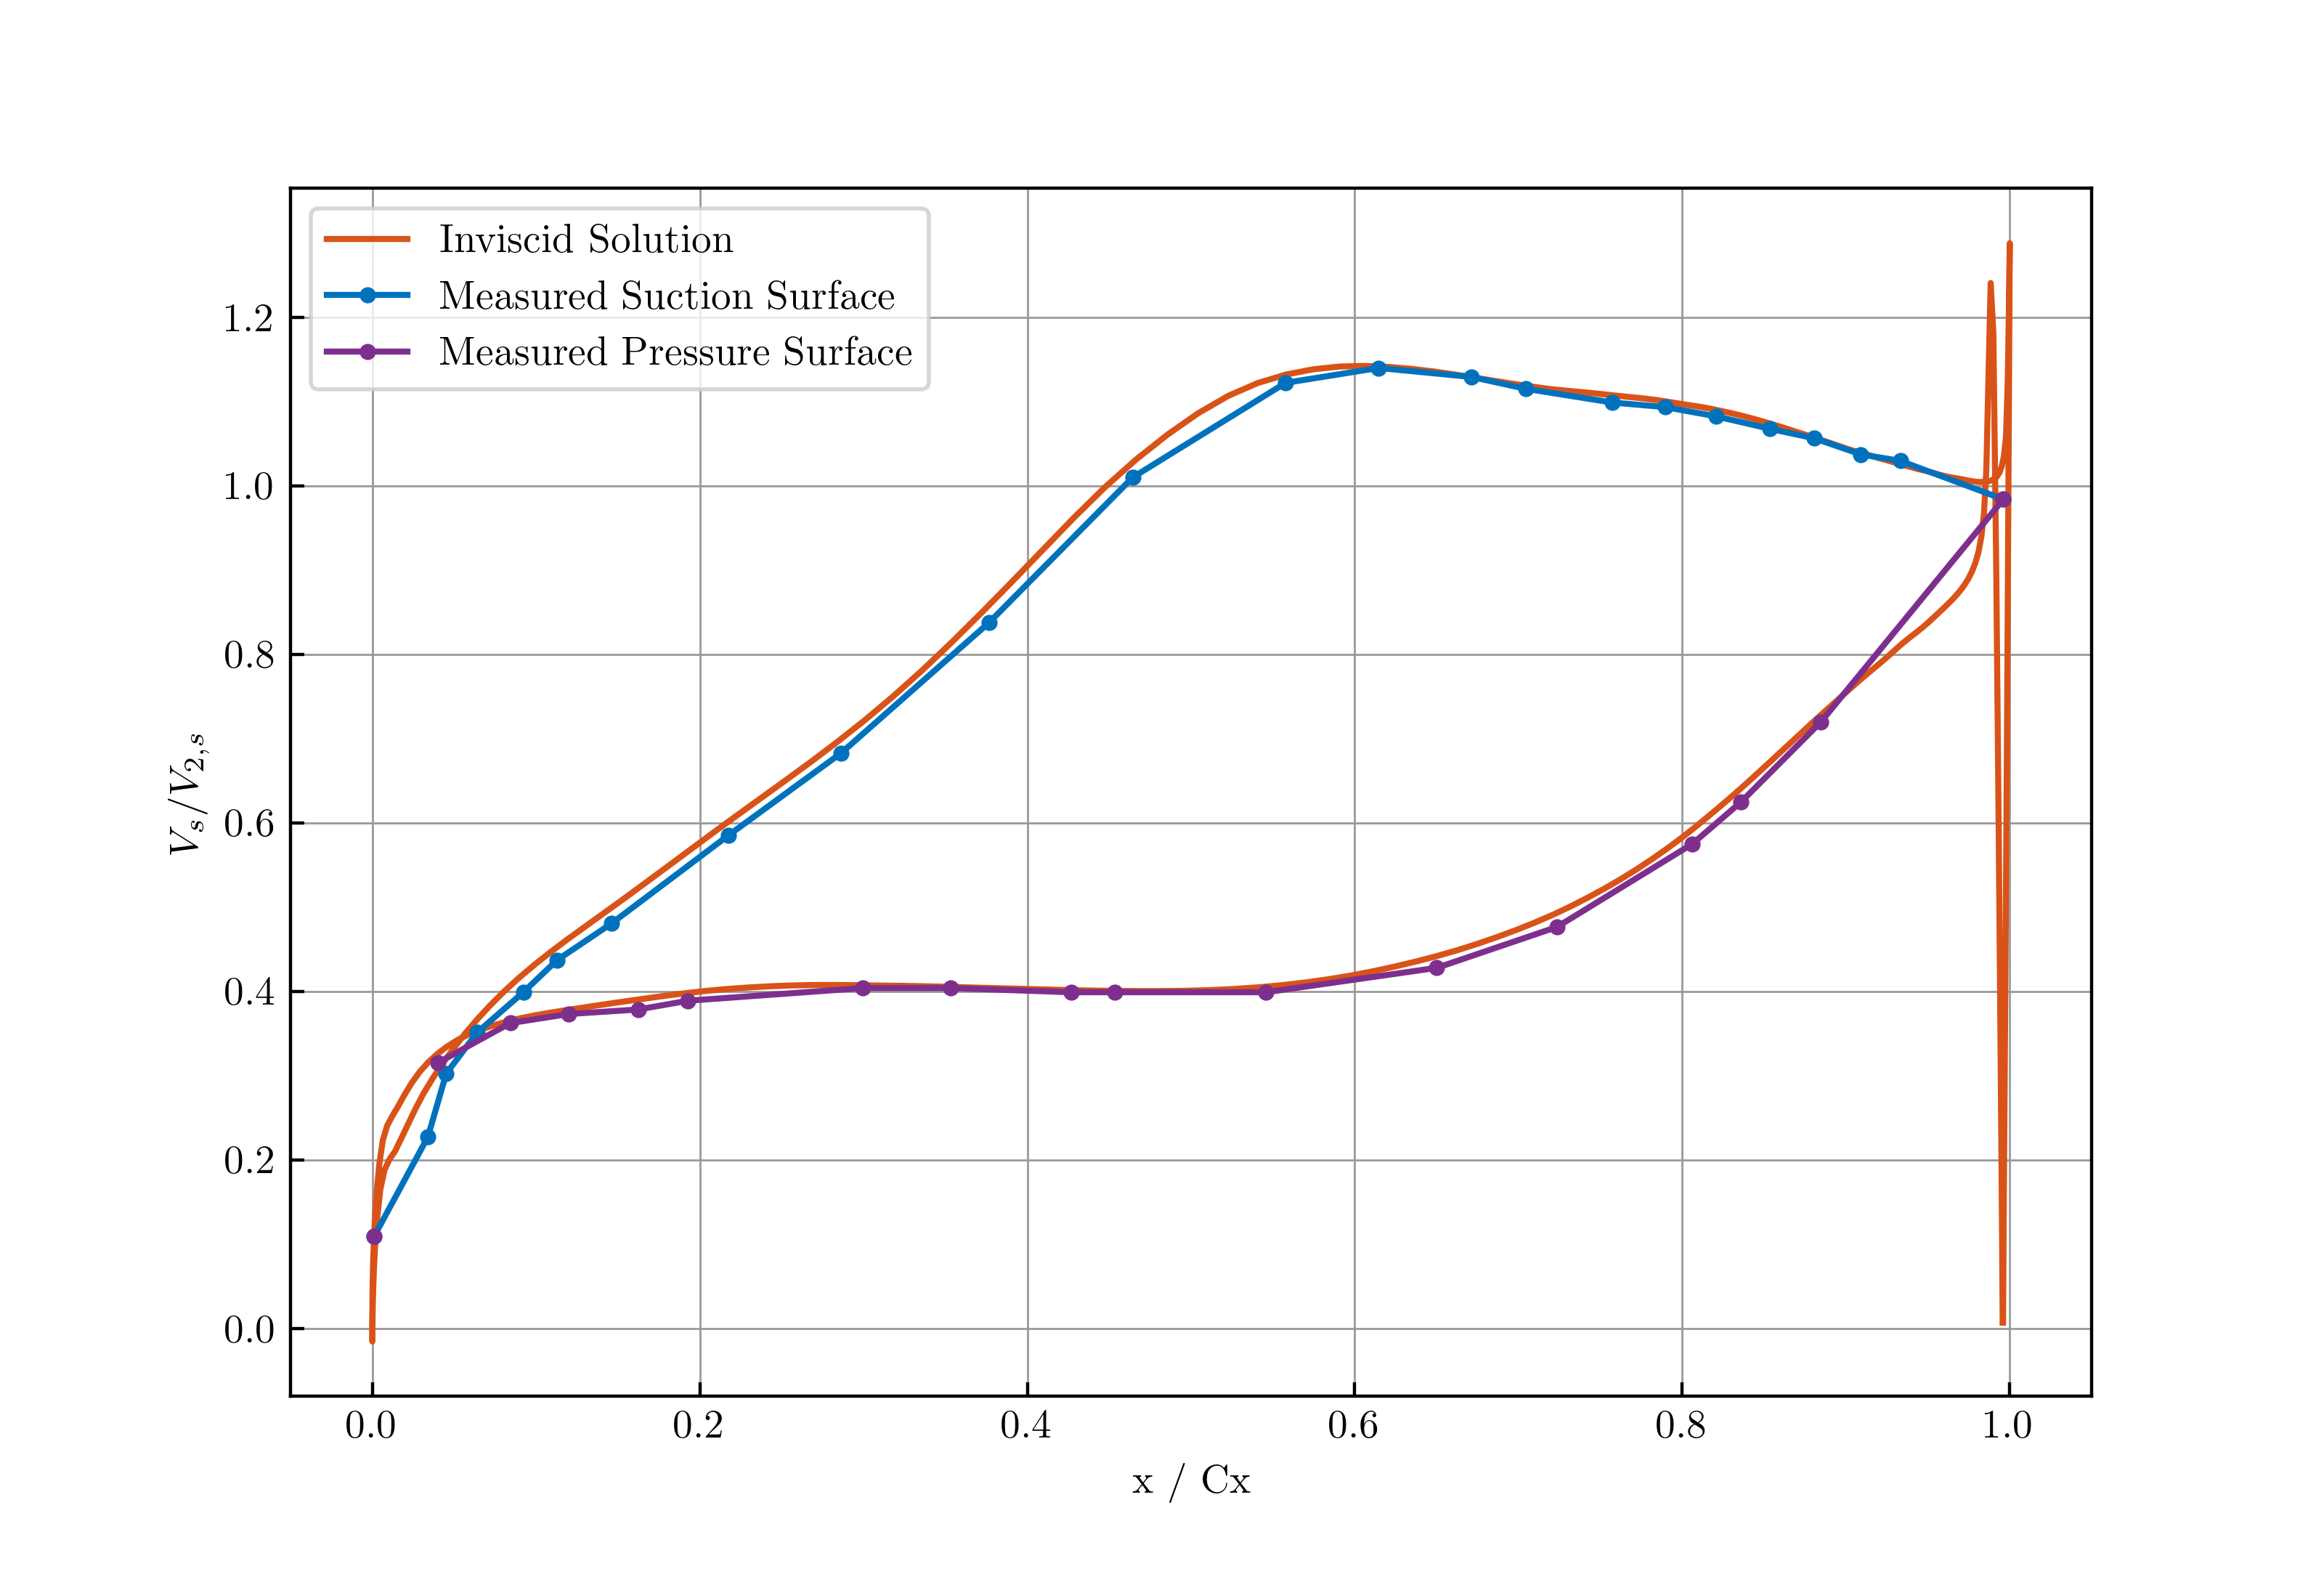
\includegraphics[width=0.7\textwidth]{figures/turbine_real.png}
    \caption{Real turbine data \cite{4A3_lab}}
    \label{fig:turbine_real}
\end{figure}

\end{document}